\chapter{Komplexität der Nominalflexion}\label{6}

In diesem Kapitel werden die Resultate aus der Messung der Komplexität in der Nominalflexion vorgestellt. Die Abfolge der Unterkapitel folgt jener aus dem Abschnitt \sectref{3.2} zu den Hypothesen: \isi{Diachronie} (\sectref{6.1}), \isi{Dialektgruppen} (\sectref{6.2}), Kontakt (\sectref{6.3}), \isi{Standardvarietät} (\sectref{6.4}) und \isi{Isolation} (\sectref{6.5}). In \sectref{6.6} werden die wichtigsten Resultate und Analysen zusammengefasst.

Es sei hier daran erinnert, dass der \isi{bestimmte Artikel} und das \isi{Demonstrativpronomen} einerseits sowie der \isi{unbestimmte Artikel} und das \isi{Possessivpronomen} andererseits jeweils zusammen eine Kategorie bilden. Begründet wird dies in \sectref{4.3.2} Des Weiteren werden der \isi{bestimmte Artikel} und das \isi{Demonstrativpronomen} mit Det1 abgekürzt (vgl. \sectref{5.5.1}), der \isi{unbestimmte Artikel} und das \isi{Possessivpronomen} mit Det2 (vgl. \sectref{5.6.1}).

\section{Diachronie}\label{6.1}

Im ersten Teil wird der Wandel im Grad der Komplexität vorgestellt, wobei diachrone Komplexifizierung und Simplifizierung festgestellt und systemintern erklärt werden. Im zweiten Teil wird gezeigt, dass es leicht mehr isolierte als nicht isolierte Dialekte gibt, die diachrone Komplexifizierung aufweisen, jedoch sind diese Unterschiede zwischen den \isi{Dialektgruppen} größer als zwischen isolierten und nicht isolierten Dialekten. Der dritte Teil widmet sich der Frage des diachronen Komplexitätsausgleichs, wobei festgehalten werden kann, dass ein solcher in der Nominalflexion der hier untersuchten Varietäten nicht vorkommt.

\subsection{Beschreibung und systeminterne Beobachtungen}\label{6.1.1}

Das hier untersuchte Sample erlaubt zwei diachrone Vergleiche: 1) Althoch-\linebreak deutsch vs. Mittelhochdeutsch, 2) Althochdeutsch/Mittelhochdeutsch vs. moderne Varietäten. Die Resultate sind in der \tabref{table6.1} (Gesamtkomplexität der Nominalflexion) und in den Tabellen \ref{table6.2}–\ref{table6.8} (Komplexität der einzelnen untersuchten Kategorien) dargestellt.

{Althochdeutsch vs. Mittelhochdeutsch:} Vergleicht man die Komplexität der Nominalflexion des Alt- und Mittelhochdeutschen, so ist festzustellen, dass sie diachron variiert. Die strukturelle Komplexität in der Flexion kann sich folglich sehr wohl diachron verändern, einen diachronen Komplexitätsausgleich gibt es zumindest in diesen beiden Varietäten des Deutschen nicht. In der Gesamtkomplexität, aber auch in allen Kategorien (mit der Ausnahme der Kategorie Det1, vgl. \tabref{table6.8}) ist Althochdeutsch komplexer als Mittelhochdeutsch. Verallgemeinernd könnte man folglich behaupten, dass Sprachen diachron an Komplexität verlieren. Dies trifft auf das Mittelhochdeutsche verglichen mit dem Althochdeutschen zu, jedoch nur bedingt auf den Vergleich mit den modernen Dialekten, was gleich anschließend erörtert wird. Eine Ausnahme von dieser generellen Tendenz bezüglich des Mittelhochdeutschen betrifft die Kategorie Det1, welche im Mittelhochdeutschen leicht komplexer ist als im Althochdeutschen. Zwar weist das Mittelhochdeutsche keinen Instrumental mehr auf (vgl. Paradigmen 81 und 82). Außerdem sind im Mittelhochdeutschen die Formen des Dativs und des Genitivs Feminin Singular wie auch das Maskulin und Neutrum im Nominativ/Akkusativ Plural zusammengefallen. Die höhere Komplexität des Mittelhochdeutschen erklärt sich durch die freien Varianten, wie z.\,B.\ im Dativ Singular Maskulin und Neutrum (mhd. \textit{dɛm}/\textit{dɛmo}) \citep[218]{Paul2007}. Bei diesen freien Varianten handelt es sich um ältere (mit Vollvokal im Nebenton, ahd. \textit{demu}, später \textit{demo}) \citep[247]{Braune2004} und neuere Formen. Dazu sind jedoch noch zwei Präzisierungen anzufügen: Erstens muss der mittelhochdeutschen Schreibung \textit{dɛmo} nicht unbedingt ein Vollvokal im Nebenton entsprechen. Jedoch unabhängig davon, exakt welche Qualität für \textit{o} angenommen wird, sind basierend auf \citet{Paul2007} für das alemannische Mittelhochdeutsch zwei Varianten festzustellen. Zweitens ist es durchaus denkbar, dass diese \isi{Variation} bereits althochdeutsche Vorläufer hatte, welche nicht verschriftlicht wurden. Weil jedoch noch nicht geklärt ist, ob für das Althochdeutsche des 9. Jhs. von zwei Varianten auszugehen ist, wird in dieser Arbeit für das Althochdeutsche von einer Variante ausgegangen. Schließlich hat das Mittelhochdeutsche im Gegensatz zum Althochdeutschen einen bestimmten und \isi{unbestimmten Artikel} grammatikalisiert, was jedoch in der Flexion nicht zu einer höheren Komplexität geführt hat, weil der \isi{bestimmte Artikel} und das \isi{Demonstrativpronomen} einerseits sowie der \isi{unbestimmte Artikel} und das \isi{Possessivpronomen} andererseits dieselben Formen bzw. \isi{Suffixe} aufweisen.

{Alt-/Mittelhochdeutsch vs. moderne Varietäten:} Unter den modernen Varietäten sind die höchstalemannischen Dialekte mit Althochdeutsch und alle übrigen Varietäten mit Mittelhochdeutsch zu vergleichen, da die höchstalemannischen Dialekte etliche Eigenschaften des Althochdeutschen erhalten haben, wie z.\,B.\ die Vollvokale im Nebenton oder die flektierten prädikativen \isi{Adjektive}, und folglich nie das mittelhochdeutsche Stadium erreicht haben (\citealt[835]{Wiesinger1983}; \citealt[153–236]{Hotzenköcherle1984}). Vergleicht man die Gesamtkomplexität der verschiedenen Varietäten, dann lässt sich diachrone Simplifizierung feststellen (\tabref{table6.1}): Alle höchstalemannischen Dialekte sind weniger komplex als Althochdeutsch und alle anderen Varietäten sind weniger komplex als Mittelhochdeutsch. Dieses erste Resultat suggeriert, dass zumindest die nominale Flexionsmorphologie im Laufe der Zeit weniger komplex wird. Diese Tendenz der diachronen Simplifizierung zeigt sich weiter im \isi{Interrogativpronomen} und im \isi{Adjektiv} (\tabref{table6.2} und \tabref{table6.3}) wie auch in der Substantivflexion, und zwar sowohl bezüglich der Gesamtkomplexität der Substantivflexion (\tabref{table6.5}) als auch bezüglich der RRs und der \isi{Flexionsklassen} (\tabref{table6.4}). Diese diachrone Simplifizierung erklärt sich vorwiegend durch die Reduktion an Kasusunterscheidungen und an Allomorphien, was je nach Dialekt mehr oder weniger stark ausgeprägt ist. Was das \isi{Interrogativpronomen} betrifft, ist festzuhalten, dass Aussagen über die Komplexitätsunterschiede problematisch sind, da diese äußerst klein ausfallen.

Zu ganz anderen Erkenntnissen kommt man, wenn die Kategorien Det1, Det2 (\tabref{table6.7} und \tabref{table6.1}) und \isi{Personalpronomen} (\tabref{table6.6}) betrachtet werden. Ungefähr die Hälfte der untersuchten Dialekte (beim Det1 sogar noch etwas mehr) weist eine höhere Komplexität als Alt- bzw. Mittelhochdeutsch auf. Wir haben es hier also mit diachroner Komplexifizierung zu tun, welche zwei Ursachen hat: erstens freie \isi{Variation} und zweitens \isi{Innovationen} in der Flexionsmorphologie. Wie bereits gezeigt wurde, ist freie \isi{Variation} in diesen Kategorien in den alemannischen Dialekten sehr weit verbreitet (vgl. \sectref{5.3.4}, \sectref{5.5.4} und \sectref{5.6.3}). Zweitens können in diesen drei Kategorien verschiedene \isi{Innovationen} beobachtet werden, was kurz skizziert werden soll. Die vier Wortarten der beiden Kategorien Det1 und Det2 weisen in den alemannischen Dialekten jeweils ein eigenes Paradigma auf, während Alt- und Mittelhochdeutsch sowie die deutsche Standardsprache nur über ein Paradigma pro Kategorie verfügen (vgl. Paradigmen 81–120). Des Weiteren zeigen einige alemannische Dialekte in den Artikeln syntaktisch bedingte Varianten: Je nachdem, ob den beiden Artikeln eine Präposition vorangeht oder nicht und ob dem \isi{bestimmten Artikel} ein \isi{Adjektiv} oder ein \isi{Substantiv} folgt, hat der Artikel eine andere Form (ausführlich dargestellt in \sectref{5.5.5} und \sectref{5.6.4}). Außerdem haben einige Dialekte im \isi{bestimmten Artikel} eine spezielle Form für possessive Kontexte grammatikalisiert (vgl. \sectref{5.5.2}). Schließlich weisen einige Dialekte unterschiedliche Paradigmen je nach \isi{Possessivpronomen} auf (vgl. \sectref{5.6.6}) sowie Wur\-zel-/Stamm\-al\-ter\-na\-tio\-nen im \isi{Possessivpronomen} (vgl. \sectref{5.6.8}). Auch das \isi{Personalpronomen} der alemannischen Dialekte hat mehr Paradigmen, da in allen alemannischen Dialekten betont/unbetont (vgl. \sectref{5.3.2}) und in einigen zusätzlich \isi{Belebtheit} (vgl. \sectref{5.3.3}) grammatikalisiert wurde. Schließlich zeigt Issime ein \textit{Additive Borrowing} (vgl. \sectref{5.3.1}). Die Phänomene der diachronen Komplexifizierung sollen hier noch etwas genauer beschrieben werden.

Bezüglich der Kategorien {Det1 und Det2} kann die diachrone Komplexifizierung durch eine stärkere Grammatikalisierung der vier Wortarten erklärt werden. Althochdeutsch hat keinen Artikel. Im Mittelhochdeutschen und in der deutschen Standardsprache zeigen der \isi{bestimmte Artikel} und das \isi{Demonstrativpronomen} dieselben Formen, der \isi{unbestimmte Artikel} und das \isi{Possessivpronomen} dieselben \isi{Suffixe}. Folglich ist für die beiden Kategorien jeweils nur ein Flexionsparadigma nötig. Anders sieht dies in den alemannischen Dialekten aus, denn die vier Wortarten weisen generell unterschiedliche Formen bzw. \isi{Suffixe} auf (ausführlich erörtert in \sectref{5.5.3} und \sectref{5.6.2}). Es braucht also deutlich mehr RRs, um die Paradigmen zu definieren. In einigen Dialekten sind wenige Formen identisch (vgl. \sectref{5.5.3} und \sectref{5.6.2}): Diese \isi{Synkretismen} können durch die RRs adäquat erfasst werden (vgl. \sectref{4.1.3.3}). Dass diese vier Wortarten in den alemannischen Dialekten eigene Paradigmen haben, kann als stärkere Grammatikalisierung dieser Wortarten interpretiert werden. Dies wird besonders mit Blick auf den \isi{bestimmten Artikel} und das \isi{Demonstrativpronomen} ersichtlich. Der \isi{bestimmte Artikel} ist aus dem \isi{Demonstrativpronomen} entstanden und zeigt in den alemannischen Dialekten aus diachroner Sicht phonologisch reduzierte Formen im Vergleich zum \isi{Demonstrativpronomen}. Außerdem kommen in einigen Dialekten bei den Artikeln noch syntaktisch bedingte Varianten dazu, deren Form ebenfalls durch RRs definiert werden muss, was höhere Komplexität bedeutet (vgl. \sectref{5.5.3} und \sectref{5.6.2}). Dasselbe gilt für die anderen bereits genannten \isi{Innovationen}: Possessiv-Artikel, unterschiedliche Flexionsparadigmen je nach \isi{Possessivpronomen} und die Stammalternationen in den \isi{Possessivpronomen}.

Im {Personalpronomen} haben erstens alle alemannischen Dialekte ein vollständiges Paradigma für das betonte \isi{Personalpronomen} und eines für das unbetonte grammatikalisiert (vgl. \sectref{5.3.2}).\footnote{Eine Ausnahme bildet Elisabethtal, das ein unbetontes \isi{Personalpronomen} nur in der 3. Person Singular Maskulin und Neutrum aufweist (vgl. \sectref{5.3.2}).} Die Formen beider Paradigmen müssen definiert werden. Somit weisen die alemannischen Dialekte eine höhere Komplexität auf als Varietäten, in denen die Formen von betonten und unbetonten \isi{Personalpronomen} nicht unterschieden werden (z.\,B.\ deutsche Standardsprache). Dieses Mehr an Formen wird z.T. wieder nivelliert, je nachdem wie ausgeprägt der Kasusabbau ist. Bereits das Alt- und Mittelhochdeutsche zeigen in der 3. Person Singular und Plural unbetonte \isi{Personalpronomen}, welche in ihrer Form von jenen des betonten \isi{Personalpronomens} abweichen. Dass die \isi{Personalpronomen} der alemannischen Dialekte vollständige unbetonte Paradigmen aufweisen, kann als Ausbau einer diachron bereits vorhandenen Kategorie interpretiert werden. Zweitens verfügen einige Dialekte im Neutrum über ein belebtes und ein unbelebtes Paradigma, wobei mit den Formen des belebten Paradigmas auf belebte weibliche Entitäten referiert wird (vgl. \sectref{5.3.3}). Im Gegensatz zum unbelebten Paradigma weist das belebte eine Akkusativform auf, die sich von der Nominativform unterscheidet.\footnote{Eine Ausnahme bildet hier der Dialekt des Sensebezirks, welcher ausführlich in \sectref{5.3.3} referiert wird.} Bei dieser Akkusativform handelt es sich um eine neue Form, also um eine \isi{Innovation}. Drittens kann im \isi{Personalpronomen} von Issime ein \textit{Additive Borrowing} gefunden werden: Im Plural gibt es neben einfachen Formen (z.\,B.\ \textit{wir}) auch zusammengesetzte Formen (z.\,B.\ \textit{wirendri}), die aus dem einfachen \isi{Personalpronomen} und dem Indefinitpronomen \textit{andere} zusammengesetzt sind (Zürrer 1999: 215) (vgl. \sectref{5.3.1}). Die frankoprovenzalischen und piemontesischen Kontaktsprachen verfügen über zusammengesetzte Formen. Der Dialekt von Issime hat jedoch nicht nur das Bildungsmuster dieser zusammengesetzten Formen übernommen, sondern diese auch in seine reiche Kasusmorphologie integriert. Zu den RRs der einfachen Formen braucht es folglich auch RRs für den zweiten Teil der zusammengesetzten Formen, was zu einer höheren Komplexität führt.

Zusammenfassend kann also festgehalten werden, dass diachrone Simplifizierung und Komplexifizierung beobachtet werden können. Der Grund für die Simplifizierung ist vor allem der Abbau an Kasusunterscheidungen wie auch die Reduktion von Allomorphie. Für die diachrone Komplexifizierung wurden drei Ursachen gefunden. Erstens sind zusätzliche Unterscheidungen grammatikalisiert worden (\isi{Innovationen}), wie die \isi{Belebtheit} im \isi{Personalpronomen} oder die Gammatikalisierung des Artikels, die in den alemannischen Dialekten weiter vorangeschritten ist als im Mittelhochdeutschen und in der deutschen Standardsprache. Zu den neu grammatikalisierten Unterscheidungen können auch die syntaktisch bedingten Varianten der Artikel gezählt werden sowie der Possessiv-Artikel, die verschiedenen Paradigmen je nach \isi{Possessivpronomen} und die Stamm-/Wur\-zel\-mo\-di\-fi\-ka\-tio\-nen im \isi{Possessivpronomen}. Zweitens wurde im \isi{Personalpronomen} der alemannischen Dialekte die Unterscheidung von betonten und unbetonten \isi{Personalpronomen} von der 3. Person (Alt- und Mittelhochdeutsch) auf die 1. und 2. Person ausgeweitet. Diese Unterscheidung wurde also in den alemannischen Dialekten ausgebaut, während sie in der deutschen Standardsprache abgebaut wurde. Drittens weist der Dialekt von Issime im \isi{Personalpronomen} ein \textit{Additive Borrowing} auf.

Auf den ersten Blick sieht es aus, als ob hier ein Komplexitätsausgleich vorliege. Dies trifft jedoch nicht zu. Erstens ist es erwartbar, dass Sprachen Teile ihrer Grammatik komplexifizieren und simplifizieren, ohne dass das eine mit dem anderen zusammenhängt. Zweitens sinkt die Komplexität nicht in einem Bereich z.\,B.\ um 5, während in einem anderen Bereich gleichzeitig die Komplexität um 5 steigt. Drittens wird nicht ein und dieselbe Kategorie, z.\,B.\ \isi{Belebtheit}, in einem Bereich aufgebaut, weil sie in einem anderen Bereich abgebaut wurde. \\

% % {\tabref{table6.1}: Gesamtkomplexität}\\

\begin{table}[h]
\caption{Gesamtkomplexität}\label{table6.1}
\begin{tabularx}{\textwidth}{XXXXr}
\lsptoprule
% % \multicolumn{5}{l}{{Gesamtkomplexität (alle Kategorien)}}\\
{DG} & {Stadt/Land} & {Isolation} & {Varietät} & {Komplexität}\\\midrule
diach & – & – & {Ahd} & {163}\\
h-st & Land & \ding{52} & Jaun & 151\\
h-st & Land & \ding{52} & Issime & 141\\
h-st & Land & \ding{55} & Uri & 136\\
h-st & Land & \ding{52} & Visperterminen & 130\\
h-st & Land & \ding{55} & Sensebezirk & 126\\
diach & – & – & {Mhd} & {123}\\
hoch & Stadt & \ding{55} & Bern & 115\\
schw & Land & \ding{55} & Petrifeld & 104\\
hoch & Land & \ding{52} & Vorarlberg & 104\\
hoch & Stadt & \ding{55} & Zürich & 103\\
oberr & Land & \ding{55} & Kaiserstuhl & 99\\
schw & Land & \ding{52} & Huzenbach & 97\\
schw & Land & \ding{55} & Saulgau & 95\\
oberr & Land & \ding{55} & \mbox{Elsass (Ebene)} & 89\\
oberr & Land & \ding{52} & Münstertal & 88\\
schw & Stadt & \ding{55} & Stuttgart & 87\\
schw & Land & \ding{55} & Elisabethtal & 87\\
oberr & Stadt & \ding{55} & Colmar & 86\\
stand & – & \ding{55} & Standard & 81\\
\lspbottomrule
\end{tabularx}
\end{table}

% % {\tabref{table6.2}: Komplexität der Interrogativpronomen}\\

\begin{table}[p]
\caption{Komplexität der Interrogativpronomen}\label{table6.2}
\begin{tabularx}{\textwidth}{XXXXr}
\lsptoprule
% % {Interrogativpronomen} &  &  &  & \\
{DG} & {Stadt/Land} & {Isolation} & {Varietät} & {Komplexität}\\\midrule
diach & – & – & {Ahd} & {6}\\
schw & Land & \ding{55} & Petrifeld & 6\\
schw & Land & \ding{52} & Huzenbach & 6\\
diach & – & – & {Mhd} & {5}\\
stand & – & \ding{55} & Standard & 5\\
schw & Land & \ding{55} & Elisabethtal & 5\\
schw & Land & \ding{55} & Saulgau & 5\\
schw & Stadt & \ding{55} & Stuttgart & 5\\
h-st & Land & \ding{52} & Issime & 4\\
h-st & Land & \ding{52} & Visperterminen & 4\\
h-st & Land & \ding{52} & Jaun & 4\\
h-st & Land & \ding{55} & Uri & 4\\
hoch & Stadt & \ding{55} & Bern & 4\\
hoch & Land & \ding{52} & Vorarlberg & 4\\
oberr & Land & \ding{55} & \mbox{Elsass (Ebene)} & 4\\
h-st & Land & \ding{55} & Sensebezirk & 3\\
hoch & Stadt & \ding{55} & Zürich & 3\\
oberr & Land & \ding{55} & Kaiserstuhl & 3\\
oberr & Land & \ding{52} & Münstertal & 3\\
oberr & Stadt & \ding{55} & Colmar & 3\\
\lspbottomrule
\end{tabularx}
\end{table}

% % {Tabelles 6.3: Komplexität der Adjektive}\\

\begin{table}[p]
\caption{Komplexität der Adjektive}\label{table6.3}
\begin{tabularx}{\textwidth}{XXXXr}
\lsptoprule
% % {Adjektiv} &  &  &  & \\
{DG} & {Stadt/Land} & {Isolation} & {Varietät} & {Komplexität}\\\midrule
diach & – & – & {Ahd} & {29}\\
diach & – & – & {Mhd} & {20}\\
h-st & Land & \ding{52} & Jaun & 15\\
h-st & Land & \ding{52} & Visperterminen & 14\\
stand & – & \ding{55} & Standard & 14\\
h-st & Land & \ding{52} & Issime & 11\\
h-st & Land & \ding{55} & Sensebezirk & 11\\
oberr & Stadt & \ding{55} & Colmar & 11\\
hoch & Stadt & \ding{55} & Bern & 10\\
hoch & Land & \ding{52} & Vorarlberg & 10\\
oberr & Land & \ding{55} & Kaiserstuhl & 10\\
schw & Stadt & \ding{55} & Stuttgart & 10\\
h-st & Land & \ding{55} & Uri & 9\\
hoch & Stadt & \ding{55} & Zürich & 9\\
schw & Land & \ding{55} & Saulgau & 8\\
oberr & Land & \ding{55} & \mbox{Elsass (Ebene)} & 8\\
oberr & Land & \ding{52} & Münstertal & 8\\
schw & Land & \ding{55} & Petrifeld & 7\\
schw & Land & \ding{55} & Elisabethtal & 7\\
schw & Land & \ding{52} & Huzenbach & 6\\
\lspbottomrule
\end{tabularx}
\end{table}

% % {\tabref{table6.4}: Anzahl der \isi{Realisierungsregeln} und \isi{Flexionsklassen} der Substantive}\\

\begin{table}[p]
\caption{Anzahl der Realisierungsregeln und Flexionsklassen der Substantive}\label{table6.4}
\footnotesize\begin{tabular}{llllr}
\lsptoprule
\multicolumn{5}{c}{{\isi{Realisierungsregeln} (\isi{Substantive})}} \\\cmidrule(lr){1-5}
{DG} & {Stadt/Land} & {Isolation} & {Varietät} & {Komplexität}\\\midrule
diach & – & – & {Ahd} & {33} \\                                       
h-st & Land & \ding{52} & Issime & 20 \\           
diach & – & – & {Mhd} & {16} \\               
h-st & Land & \ding{52} & Visperterminen & 15  \\  
h-st & Land & \ding{52} & Jaun & 12  \\            
h-st & Land & \ding{55} & Uri & 12 \\            
schw & Land & \ding{55} & Petrifeld & 10 \\      
stand & – & \ding{55} & Standard & 9 \\          
h-st & Land & \ding{55} & Sensebezirk & 8 \\     
hoch & Stadt & \ding{55} & Zürich & 8      \\      
oberr & Land & \ding{52} & Münstertal & 8    \\    
oberr & Land & \ding{55} & Kaiserstuhl & 7 \\    
schw & Land & \ding{55} & Saulgau & 7  \\        
hoch & Land & \ding{52} & Vorarlberg & 6 \\        
schw & Land & \ding{52} & Huzenbach & 6  \\        
schw & Land & \ding{55} & Elisabethtal & 6    \\   
hoch & Stadt & \ding{55} & Bern & 5\\            
oberr & Land & \ding{55} & Elsass (Ebene) & 5 \\ 
schw & Stadt & \ding{55} & Stuttgart & 4 \\      
oberr & Stadt & \ding{55} & Colmar & 4   \\      
\midrule
\multicolumn{5}{c}{{Flexionsklassen}}\\\cmidrule(lr){1-5}
{DG} & {Stadt/Land} & {Isolation} & {Varietät} & {Komplexität}\\\midrule
diach & – & – & {Ahd} & {19}\\
h-st & Land & \ding{52} & Issime & 18\\
h-st & Land & \ding{52} & Visperterminen & 18\\
h-st & Land & \ding{52} & Jaun & 16\\
h-st & Land & \ding{55} & Uri & 12\\
diach & – & – & {Mhd} & {11}\\
schw & Land & \ding{55} & Elisabethtal & 11\\
stand & – & \ding{55} & Standard & 10\\
h-st & Land & \ding{55} & Sensebezirk & 10\\
schw & Land & \ding{55} & Petrifeld & 9\\
hoch & Stadt & \ding{55} & Zürich & 8\\
oberr & Land & \ding{55} & Elsass (Ebene) & 8\\
hoch & Stadt & \ding{55} & Bern & 7\\
hoch & Land & \ding{52} & Vorarlberg & 7\\
oberr & Land & \ding{52} & Münstertal & 7\\
schw & Land & \ding{52} & Huzenbach & 6\\
schw & Land & \ding{55} & Saulgau & 6\\
oberr & Land & \ding{55} & Kaiserstuhl & 5\\
schw & Stadt & \ding{55} & Stuttgart & 5\\      
\lspbottomrule
\end{tabular}
\end{table}

% % {\tabref{table6.5}: Komplexität der Substantive}\\

\begin{table}[p]
\caption{Komplexität der Substantive}\label{table6.5}
\begin{tabularx}{\textwidth}{XXXXr}
\lsptoprule
\multicolumn{5}{c}{{\isi{Substantive} (\isi{Realisierungsregeln} + \isi{Flexionsklassen})}}  \\
{DG} & {Stadt/Land} & {Isolation} & {Varietät} & {Komplexität}\\\midrule
diach & – & – & {Ahd} & {52}\\
h-st & Land & \ding{52} & Issime & 38\\
h-st & Land & \ding{52} & Visperterminen & 33\\
h-st & Land & \ding{52} & Jaun & 28\\
diach & – & – & {Mhd} & {27}\\
h-st & Land & \ding{55} & Uri & 24\\
stand & – & \ding{55} & Standard & 19\\
schw & Land & \ding{55} & Petrifeld & 19\\
h-st & Land & \ding{55} & Sensebezirk & 18\\
schw & Land & \ding{55} & Elisabethtal & 17\\
hoch & Stadt & \ding{55} & Zürich & 16\\
oberr & Land & \ding{52} & Münstertal & 15\\
oberr & Land & \ding{55} & \mbox{Elsass (Ebene)} & 13\\
hoch & Land & \ding{52} & Vorarlberg & 13\\
schw & Land & \ding{55} & Saulgau & 13\\
hoch & Stadt & \ding{55} & Bern & 12\\
schw & Land & \ding{52} & Huzenbach & 12\\
oberr & Land & \ding{55} & Kaiserstuhl & 12\\
schw & Stadt & \ding{55} & Stuttgart & 9\\
oberr & Stadt & \ding{55} & Colmar & 9\\
\lspbottomrule
\end{tabularx}
\end{table}

% % {\tabref{table6.6}: Komplexität der Personalpronomen}\\

\begin{table}[p]
\caption{Komplexität der Personalpronomen}\label{table6.6}
\begin{tabularx}{\textwidth}{XXXXr}
\lsptoprule
% % \multicolumn{5}{c}{{Personalpronomen}}  \\
{DG} & {Stadt/Land} & {Isolation} & {Varietät} & {Komplexität}\\\midrule
h-st & Land & \ding{52} & Jaun & 55\\
h-st & Land & \ding{52} & Issime & 52\\
h-st & Land & \ding{55} & Uri & 51\\
h-st & Land & \ding{55} & Sensebezirk & 49\\
hoch & Stadt & \ding{55} & Bern & 46\\
diach & – & – & {Ahd} & {45}\\
h-st & Land & \ding{52} & Visperterminen & 45\\
schw & Land & \ding{52} & Huzenbach & 42\\
hoch & Land & \ding{52} & Vorarlberg & 41\\
diach & – & – & {Mhd} & {39}\\
hoch & Stadt & \ding{55} & Zürich & 39\\
schw & Land & \ding{55} & Petrifeld & 37\\
oberr & Land & \ding{55} & Kaiserstuhl & 37\\
oberr & Land & \ding{52} & Münstertal & 37\\
oberr & Land & \ding{55} & \mbox{Elsass (Ebene)} & 36\\
oberr & Stadt & \ding{55} & Colmar & 36\\
schw & Stadt & \ding{55} & Stuttgart & 36\\
schw & Land & \ding{55} & Saulgau & 35\\
schw & Land & \ding{55} & Elisabethtal & 29\\
stand & – & \ding{55} & Standard & 24\\
\lspbottomrule
\end{tabularx}
\end{table}

% % {\tabref{table6.7}: Komplexität des \isi{unbestimmten Artikels}/} {Possessivpronomens}\\


\begin{table}[p]
\caption{Komplexität des unbestimmten Artikels/Possessivpronomens}\label{table6.7}
\begin{tabularx}{\textwidth}{XXXXr}
\lsptoprule
% % \multicolumn{5}{l}{{\isi{unbestimmter Artikel}/Possessivpronomen}}  \\
{DG} & {Stadt/Land} & {Isolation} & {Varietät} & {Komplexität}\\\midrule
h-st & Land & \ding{55} & Sensebezirk & 30\\
h-st & Land & \ding{52} & Jaun & 29\\
h-st & Land & \ding{55} & Uri & 29\\
hoch & Stadt & \ding{55} & Bern & 26\\
oberr & Land & \ding{55} & Kaiserstuhl & 22\\
hoch & Stadt & \ding{55} & Zürich & 21\\
h-st & Land & \ding{52} & Issime & 19\\
schw & Land & \ding{55} & Petrifeld & 19\\
diach & – & – & {Ahd} & {17}\\
diach & – & – & {Mhd} & {16}\\
schw & Land & \ding{55} & Saulgau & 16\\
hoch & Land & \ding{52} & Vorarlberg & 16\\
h-st & Land & \ding{52} & Visperterminen & 12\\
oberr & Land & \ding{55} & \mbox{Elsass (Ebene)} & 12\\
schw & Land & \ding{52} & Huzenbach & 12\\
schw & Land & \ding{55} & Elisabethtal & 12\\
schw & Stadt & \ding{55} & Stuttgart & 11\\
oberr & Land & \ding{52} & Münstertal & 11\\
oberr & Stadt & \ding{55} & Colmar & 9\\
stand & – & \ding{55} & Standard & 8\\
\lspbottomrule
\end{tabularx}
\end{table}

% {\tabref{table6.8}: Komplexität des \isi{bestimmten Artikels}/Demonstrativpronomens}\\

\begin{table}[p]
\caption{Komplexität des bestimmten Artikels/Demonstrativpronomens}\label{table6.8}
\begin{tabularx}{\textwidth}{XXXXr}
\lsptoprule
% % \multicolumn{5}{l}{{\isi{bestimmter Artikel}/Demonstrativpronomen}}  \\
{DG} & {Stadt/Land} & {Isolation} & {Varietät} & {Komplexität}\\\midrule
h-st & Land & \ding{52} & Visperterminen & 22\\
h-st & Land & \ding{52} & Jaun & 20\\
h-st & Land & \ding{55} & Uri & 19\\
hoch & Land & \ding{52} & Vorarlberg & 20\\
schw & Land & \ding{52} & Huzenbach & 19\\
schw & Land & \ding{55} & Saulgau & 18\\
oberr & Stadt & \ding{55} & Colmar & 18\\
h-st & Land & \ding{52} & Issime & 17\\
hoch & Stadt & \ding{55} & Bern & 17\\
schw & Land & \ding{55} & Elisabethtal & 17\\
diach & – & – & {Mhd} & {16}\\
schw & Stadt & \ding{55} & Stuttgart & 16\\
schw & Land & \ding{55} & Petrifeld & 16\\
oberr & Land & \ding{55} & \mbox{Elsass (Ebene)} & 16\\
diach & – & – & {Ahd} & {15}\\
h-st & Land & \ding{55} & Sensebezirk & 15\\
hoch & Stadt & \ding{55} & Zürich & 15\\
oberr & Land & \ding{55} & Kaiserstuhl & 15\\
oberr & Land & \ding{52} & Münstertal & 14\\
stand & – & \ding{55} & Standard & 11\\
\lspbottomrule
\end{tabularx}
\end{table}
\clearpage

\subsection{Variation der strukturellen Komplexität und Isolation}\label{6.1.2}

Es wurde gezeigt, dass in allen untersuchten Dialekten die Komplexität der Sub\-stan\-tiv- und Adjektivflexion diachron gesunken ist. Jedoch weisen einige Dialekte in der Flexion des \isi{Personalpronomens}, des Det1 und Det2 diachron höhere Komplexität auf. Es stellt sich also die Frage, ob dies durch soziolinguistische Faktoren erklärt werden kann bzw. was jene Dialekte gemeinsam haben, die diachrone Komplexifizierung zeigen.

Laut \citet{Trudgill2011} müssten gerade kleine und \isi{isolierte Sprachgemeinschaften} höhere Komplexität aufweisen: Erstens erhalten diese Sprachgemeinschaften zu einem höheren Maß strukturelle Komplexität, und zweitens kommt jene Art des Sprachwandels, die die strukturelle Komplexität erhöht, eher in diesen Sprachgemeinschaften vor (detailliert dargestellt in \sectref{2.2.3}, vgl. \sectref{3.2.1} zu den Hypothesen). In diesem Sample müssten also vor allem die sechs isolierten Varietäten diachrone Komplexifizierung zeigen. Um dies zu überprüfen, wurde erstens gezählt, wie viele dieser sechs isolierten und wie viele der zwölf nicht isolierten Varietäten in den drei Kategorien (mit diachroner Komplexifizierung) durchschnittlich diachrone Komplexifizierung aufweisen, d.h., wie viele der isolierten und nicht isolierten Dialekte höhere Komplexität als ihr diachrones Pendant zeigen (vgl. Tabellen \ref{table6.6}–\ref{table6.8}). Das diachrone Pendant der höchstalemannischen Dialekte ist das Althochdeutsche, für alle anderen Varietäten das Mittelhochdeutsche (vgl. \sectref{6.1.1}). Die Resultate sind in \tabref{table6.9} zusammengefasst, und zwar in der ersten Zeile (z.\,B.\ 4/6 ({\textasciitilde}66\%)). In den drei Kategorien, in denen diachrone Komplexifizierung vorkommt, zeigen durchschnittlich 61\% der isolierten Varietäten und durchschnittlich 47\% der nicht isolierten Varietäten diachrone Komplexifizierung. Diachrone Komplexifizierung kommt also tendenziell etwas häufiger in isolierten als in nicht isolierten Varietäten vor.

Zweitens wurde das Ausmaß der Komplexifizierung bzw. Simplifizierung identifiziert, indem die Abweichung einer Varietät von ihrem diachronen Pendant berechnet wurde (Komplexifizierungswert). Beispielsweise hat der Dialekt von Huzenbach im \isi{Personalpronomen} die Komplexität 42, der Dialekt von Stuttgart die Komplexität 36 und Mittelhochdeutsch die Komplexität 39. Der Dialekt von Huzenbach weist also einen Komplexifizierungswert von +3 auf, der Dialekt von Stuttgart einen Komplexifizierungswert von –3. Diese Resultate sind in der zweiten Zeile der \tabref{table6.9} dargestellt. In allen Kategorien wird stärker komplexifiziert als simplifiziert (positive Zahlen) außer im \isi{Personalpronomen} der nicht isolierten Dialekte (negative Zahl). Die isolierten Dialekte komplexifizieren jedoch in jeder Kategorie stärker als die nicht isolierten Dialekte. Durchschnittlich zeigen die isolierten Dialekte einen höheren Komplexifizierungswert (+2,56) als die nicht isolierten Dialekte (+0,5). Dies untermauert also die oben diskutierten Resultate.

% % {\tabref{table6.9}: Anzahl (nicht) isolierte Dialekte mit diachroner Komplexifizierung und Komplexifizierungswert}\\

\begin{table}[t]
\caption{Anzahl (nicht) isolierter Dialekte mit diachroner Komplexifizierung und Komplexifizierungswert}\label{table6.9}
\begin{tabularx}{\textwidth}{XXXXX}
\lsptoprule
& Personal-pronomen & unbest. Artikel / \isi{Possessivpronomen} & \mbox{best. Artikel /} \isi{Demonstrativpronomen} & Durchschnitt\\
\midrule
+ isoliert & 4/6 ({\textasciitilde}66\%)

+3,34 & 2/6 ({\textasciitilde}33\%)

+1,17 & 5/6 ({\textasciitilde}83\%)

+3,17 & 11/18 ({\textasciitilde}61\%)

+2,56\\

\midrule
– isoliert & 3/12 (25\%)

–2,08 & 6/12 (50\%)

+3,42 & 8/12 ({\textasciitilde}66\%)

+0,17 & 17/36 ({\textasciitilde}47\%)

+0,5\\
\lspbottomrule
\end{tabularx}
\end{table}

Eine klarere Tendenz kann gefunden werden, wenn das gleiche Prozedere auf die \isi{Dialektgruppen} angewendet wird. Die Resultate stehen in \tabref{table6.10}. Von den fünf höchstalemannischen Dialekten zeigen durchschnittlich 80\% diachrone Komplexifizierung, von den drei hochalemannischen Dialekten ca. 66\%, von den fünf schwäbischen Dialekten ca. 33\% und von den vier oberrheinalemannischen Dialekten ca. 17\%. Die deutsche Standardsprache ist in allen drei Kategorien weniger komplex als das Mittelhochdeutsche. Diachrone Komplexifizierung kann also noch besser durch den Faktor \isi{Dialektgruppe} als durch den Faktor \isi{Isolation} erklärt werden.

Aufschlussreich ist hier auch der Komplexifizierungswert, also das Ausmaß der Komplexifizierung und Simplifizierung. Während die höchst- und hochalemannischen Dialekte komplexifizieren (positive Zahlen) (Höchstalemannisch mehr als Hochalemannisch), simplifizieren die schwäbischen und oberrheinalemannischen Dialekte (negative Zahlen) (Oberrheinalemannisch mehr als Schwäbisch). Eine Ausnahme bildet nur der Det1 im Schwäbischen. Die deutsche Standardsprache simplifiziert vergleichsweise in besonders starkem Maße.

% % {\tabref{table6.10}: Anzahl Dialekte pro \isi{Dialektgruppe} mit diachroner Komplexifizierung und Komplexifizierungswert}\\

\begin{table}
\caption{Anzahl von Dialekten pro Dialektgruppe mit diachroner Komplexifizierung und Komplexifizierungswert}\label{table6.10}
\begin{tabularx}{\textwidth}{XXXXX}
\lsptoprule
DG & Personal-pronomen & unbest. Artikel /  \isi{Possessivpronomen} & \mbox{best. Artikel /} \isi{Demonstrativpronomen} & Durchschnitt\\
\midrule
h-st & 4/5 (80\%)

+5,4 & 4/5 (80\%)

+12,8 & 4/5 (80\%)

+3,6 & 4/5 (80\%)

+7,27\\

\midrule
hoch & 2/3 ({\textasciitilde}66\%)

+3 & 2/3 ({\textasciitilde}66\%)

+7,5 & 2/3 ({\textasciitilde}66\%)

+1,34 & 2/3 ({\textasciitilde}66\%)

+3,95\\

\midrule
schw & 1/5 (20\%)

–3,2 & 1/5 (20\%)

–2 & 3/5 (60\%)

+1,2 & 1/3 ({\textasciitilde}33\%)

–1,34\\

\midrule
oberr & 0/4 (0\%)

–2,5 & 1/4 (25\%)

–3 & 1/4 (25\%)

–0,25 & 1/6 ({\textasciitilde}17\%)

–1,92\\

\midrule
stand & 0/1 (0\%)

–15 & 0/1 (0\%)

–8 & 0/1 (0\%)

–6 & 0/1 (0\%)

–9,67\\
\lspbottomrule
\end{tabularx}
\end{table}

Um noch genauere Aussagen diesbezüglich machen zu können, wurde für jeden Dialekt gezählt, in wie vielen der drei Kategorien (\isi{Personalpronomen}, Det1, Det2) er diachrone Komplexifizierung zeigt. Vorher wurde also die Anzahl von Varietäten mit höherer Komplexität als ihr diachrones Pendant ermittelt sowie der Komplexifizierungswert. Nun werden die Anzahl von Kategorien mit diachroner Komplexifizierung pro Varietät berechnet. Anschließend wurde für jede \isi{Dialektgruppe} die durchschnittliche Anzahl komplexifizierter Kategorien ermittelt (vgl. \tabref{table6.11}). Die höchstalemannischen Dialekte weisen 2,4 Kategorien (von 3 Kategorien) mit diachroner Komplexifizierung auf, die hochalemannischen Dialekte 2 Kategorien, die schwäbischen Dialekte 1 Kategorie und die oberrheinalemannischen Dialekte 0,5. Es könnte nun moniert werden, dass isolierte und nicht isolierte Dialekte nicht gleichmäßig auf alle \isi{Dialektgruppen} verteilt sind, was stimmt. Vergleicht man jedoch isolierte und nicht isolierte Dialekte innerhalb der \isi{Dialektgruppen}, zeigt sich auch da, dass nicht unbedingt die isolierten Dialekte mehr diachron komplexifizierte Kategorien aufweisen als die nicht isolierten Dialekte. Beispielsweise haben zwar Jaun und Issime (beide isoliert) alle drei Kategorien komplexifiziert, dies gilt jedoch auch für Uri (nicht isoliert), aber nicht für Visperterminen (isoliert). Diachrone Komplexifizierung ist also vor allem ein Phänomen der hoch- und höchstalemannischen Dialekte, worauf in \sectref{6.5} noch genauer eingegangen wird.\\

% {\tabref{table6.11}: Anzahl diachron komplexifizierter Kategorien}\\

\begin{table}
\caption{Anzahl diachron komplexifizierter Kategorien}\label{table6.11}
\begin{tabular}{lllrS}
\lsptoprule
{Dialekt} & {DG} & {Isoliertheit} & \multicolumn{1}{p{2cm}}{Anzahl komplexifizierter Kategorien} & \multicolumn{1}{l}{Durchschnitt}\\\midrule
Jaun & h-st & isol & 3 & 2,4\\
Issime & h-st & isol & 3 & \\
Visperterminen & h-st & isol & 1 & \\
Uri & h-st & n-isol & 3 & \\
Sensebezirk & h-st & n-isol & 2 & \\
Vorarlberg & hoch & isol & 2 & 2\\
Bern & hoch & n-isol & 3 & \\
Zürich & hoch & n-isol & 1 & \\
Huzenbach & schw & isol & 2 & 1\\
Saulgau & schw & n-isol & 1 & \\
Petrifeld & schw & n-isol & 1 & \\
Elisabethtal & schw & n-isol & 1 & \\
Stuttgart & schw & n-isol & 0 & \\
Münstertal & oberr & isol & 0 & 0,5\\
Kaiserstuhl & oberr & n-isol & 1 & \\
Colmar & oberr & n-isol & 1 & \\
Elsass (Ebene) & oberr & n-isol & 0 & \\
\lspbottomrule
\end{tabular}
\end{table}

\subsection{Zurück zum Flexionssystem: Archaismen, Innovationen und Komplexitätsausgleich}\label{6.1.3}

Zusammenfassend wurde bis jetzt Folgendes festgestellt. Erstens zeigen die modernen Varietäten diachron Simplifizierung in der Gesamtkomplexität der Nominalflexion sowie im \isi{Substantiv} und im \isi{Adjektiv}. Dies konnte durch den Kasusabbau und durch die Reduktion der Allomorphie erklärt werden. Die \isi{Interrogativpronomen} wurden ausgelassen, da die Komplexitätsunterschiede sehr klein ausfallen. Zweitens weisen einige alemannische Dialekte diachrone Komplexifizierung in drei Kategorien auf, und zwar im \isi{Personalpronomen}, im Det1 und Det2. Drittens gibt es leicht mehr isolierte als nicht isolierte Dialekte mit diachroner Komplexifizierung (vgl. \tabref{table6.9}). Deutlich größer sind jedoch die Unterschiede zwischen den \isi{Dialektgruppen}: Die meisten Dialekte mit diachroner Komplexifizierung hat das Höchstalemannische, gefolgt von Hochalemannisch, Schwäbisch, Oberrheinalemannisch und der Standardsprache (keine diachrone Komplexifizierung) (vgl. Tabellen \ref{table6.10}–\ref{table6.11}).

Was noch nicht diskutiert wurde, ist das Verhältnis zwischen \isi{Innovationen} und \isi{Archaismen}. Es stellt sich also die Frage, was das Verhältnis ist zwischen Erhalt oder Abbau von struktureller Komplexität einerseits und \isi{Innovationen}, die zu einer höheren Komplexität führen, oder Fehlen von \isi{Innovationen} andererseits. Beispielsweise kann eine neue Kategorie in allen Varietäten grammatikalisiert werden (z.\,B.\ Artikel), es macht jedoch bezüglich der Komplexität der Flexion einen Unterschied, ob diese neue Kategorie in ein neues drei-Kasus-System oder in ein altes vier-Kasus-System integriert wird. Mit den zwei Variablen ‘\isi{Innovation}’ (hier gebraucht im Sinne von Komplexifizierung, komplexitätsaufbauend) und ‘\isi{Archaismus}’ (im Sinne von Erhalt von Komplexität, komplexitätserhaltend) lassen sich theoretisch vier Typen bilden: 1) \isi{Innovationen} und \isi{Archaismen}, 2) \isi{Innovationen} und keine \isi{Archaismen} (=Simplifizierung), 3) keine \isi{Innovationen} und \isi{Archaismen}, 4) keine \isi{Innovationen} und keine \isi{Archaismen}.

In der Folge soll nun auf zwei Punkte eingegangen werden. Zuerst werden die diachron komplexifizierten Kategorien nochmal detaillierter betrachtet. Es wird gezeigt, dass sich die \isi{Dialektgruppen} in ihrer Innovationsrate klar unterscheiden und alle vier Typen der zwei Variablen ‘\isi{Innovation}’ und ‘\isi{Archaismus}’ vorkommen. Anschließend sollen einige Überlegungen zum gesamten nominalen Flexionssystem angestellt werden. Vor allem wird hinterfragt, ob der Wandel zu einer kooperativen Flexion (verbunden mit der Grammatikalisierung des Artikels und der festen Abfolge innerhalb der Nominalphrase) als generelles Prinzip für die deutsche Sprache gelten kann. Dass dem nicht so ist, kann vor allem an der redundanten Kasusmarkierung in den isolierten höchstalemannischen Dialekten gezeigt werden wie auch am fehlenden Komplexitätsausgleich zwischen den Determinierern und dem \isi{Substantiv}.

{\isi{Innovationen} und \isi{Archaismen}:} In der hier verwendeten Methode zur Messung der Komplexität in der Flexion werden Auf- und Abbau von Komplexität miteinander verrechnet. Dies ist auch erwünscht, da nur so Aussagen und Vergleiche zur Höhe der strukturellen Komplexität gemacht werden können. Trotzdem sollen hier \isi{Innovationen} und \isi{Archaismen} nochmal genauer betrachtet werden, um das Verhältnis zwischen diesen beiden Prozessen besser zu verstehen.

Es wird dazu ein Innovationsindex errechnet, und zwar für jede \isi{Dialektgruppe} und jede Kategorie, die diachrone Komplexifizierung aufweisen (\isi{Personalpronomen}, Det1 und Det2). Zuerst wird für jede dieser Kategorien geprüft, welche \isi{Innovationen} sie zeigen (die Tabellen \ref{table6.13}–\ref{table6.16} dazu befinden sich zusammen unten):

\begin{itemize}
\item
Im \isi{Personalpronomen}: \isi{Betontheit} (\sectref{5.3.2}), \isi{Belebtheit} (\sectref{5.3.3}) und das \textit{Additive Borrowing} (nur in Issime) (\sectref{5.3.1}) (vgl. \tabref{table6.13}).
\item
Im Det1: Possessiv-Artikel (\sectref{5.5.2}), syntaktisch bedingte \isi{Variation} des \isi{bestimmten Artikels} (±vorangehende Präposition) im Akkusativ und/oder Dativ (\sectref{5.5.5}), syntaktisch bedingte \isi{Variation} des \isi{bestimmten Artikels} vor \isi{Adjektiv} und \isi{Substantiv} (\sectref{5.5.5}) (vgl. \tabref{table6.14}).
\item
Im Det2: Syntaktisch bedingte \isi{Variation} des \isi{unbestimmten Artikels} (±vorangehende Präposition) im Akkusativ und/oder Dativ (\sectref{5.6.4} und \sectref{5.6.5}), unterschiedliche Paradigmen abhängig vom \isi{Possessivpronomen} (\sectref{5.6.6}), Wur\-zel-/Stamm\-al\-ter\-na\-tio\-nen im \isi{Possessivpronomen} (\sectref{5.6.8}) (vgl. \tabref{table6.15}).
\end{itemize}

Die Grammatikalisierung des Artikels wird nicht berücksichtigt, da alle untersuchten Dialekte einen bestimmten und \isi{unbestimmten Artikel} grammatikalisiert haben und dieser sich von der Flexion des \isi{Demonstrativpronomens} bzw. des \isi{Possessivpronomens} unterscheidet (vgl. \sectref{5.5.3} und \sectref{5.6.2}). Anschließend wird für jeden Dialekt gezählt, wie viele dieser \isi{Innovationen} er aufweist und schließlich wie viele \isi{Innovationen} jede \isi{Dialektgruppe} durchschnittlich hat (Tabellen \ref{table6.13}–\ref{table6.15}). Eine Übersicht über alle \isi{Innovationen} der drei Kategorien gibt \tabref{table6.16}, in der die \isi{Innovationen} in den drei Kategorien addiert sind.

Betrachtet man die gesamte Komplexifizierungsrate (=Innovationsindex, komplexitätsaufbauend) (\tabref{table6.16}), so stellt man fest, dass die höchst- und hochalemannischen Dialekte deutlich mehr \isi{Innovationen} (ca. 6) aufweisen als die oberrheinalemannischen und schwäbischen Dialekte (ca. 3). Des Weiteren sind die höchstalemannischen Dialekte besonders auffällig, weil es einen großen Innovationsunterschied nicht zwischen den isolierten und den nicht isolierten Dialekten gibt, sondern zwischen den Walser- und den Nicht-Wal\-ser\-di\-a\-lek\-ten. Deswegen werden deren Innovationsraten nochmal getrennt berechnet. Dabei zeigt sich, dass die Walser Dialekte ähnlich wenig innovativ sind wie die oberrheinalemannischen und schwäbischen Dialekte (3), während die nicht-Walser höchstalemannischen Dialekte eine etwas höhere Innovationsrate (8,33) als die hochalemannischen Dialekte (6,33) haben. Dasselbe Muster zeigt sich auch dann, wenn man die drei Kategorien getrennt betrachtet (Tabellen \ref{table6.13}–\ref{table6.15}). Folglich gibt es \isi{Dialektgruppen}, die deutlich innovativer (=komplexitätsaufbauend) sind als andere. Verallgemeinernd können sie in drei Gruppen eingeteilt werden: sehr innovativ (nicht-Walser Höchstalemannisch), innovativ (Hochalemannisch), wenig innovativ (Walser Höchstalemannisch, Oberrheinalemannisch, Schwäbisch).

Noch interessanter wird dies, vergleicht man diese Resultate mit dem Kasuserhalt und -abbau in den drei Kategorien (Tabellen \ref{table6.13}–\ref{table6.15}), wobei es sich wohl um den wichtigsten Wandel in die entgegengesetzte Richtung handelt, nämlich in Richtung Simplifizierung. Hierzu muss noch erwähnt werden, dass in diesen drei Kategorien das Althochdeutsche einen Instrumental nur noch im Maskulin/Neutrum Singular des Demonstrativ- und \isi{Possessivpronomens} hat, weswegen auch für das Althochdeutsche in diesem Abschnitt verallgemeinert von vier \isi{Kasus} ausgegangen wird. Generell kann man feststellen, dass die isolierten höchstalemannischen Dialekte (Issime, Visperterminen und Jaun) ein vier-Kasus-System erhalten haben (=\isi{Archaismus}), während die übrigen Dialekte über ein drei-Kasus-System verfügen.\footnote{Der Dialekt des Sensebezirks und von Uri zeigen Genitive nur im betonten \isi{Personalpronomen}, der Dialekt des Sensebezirks zusätzlich nur eine Form im Genitiv Plural unbetont (vgl. Paradigmen 47 und 48).}

Werden nun die Innovativität (\tabref{table6.16}) und der Kasuserhalt/-abbau verglichen, können folgende fünf Typen gefunden werden:

% % {\tabref{table6.12}: \isi{Innovationen} und \isi{Archaismen} in den alemannischen Dialekten}\\

\begin{table}
\caption{Innovationen und Archaismen in den alemannischen Dialekten}\label{table6.12}
\begin{tabular}{llll}
\lsptoprule
{Typ} & {Kasus} & \multicolumn{1}{p{2.75cm}}{{Innovativität (komplexitäts-aufbauend)}} & {Dialekt}\\
\midrule
1 & Erhalt & wenig innovativ & Walser Dialekte\\
% % \midrule
2 & Erhalt & sehr innovativ & Jaun\\
% % \midrule
3 & Abbau & sehr innovativ & Sensebezirk, Uri\\
% % \midrule
4 & Abbau & innovativ & Hochalemannisch\\
% % \midrule
5 & Abbau & wenig innovativ & Oberrheinalemannisch, Schwäbisch\\
\lspbottomrule
\end{tabular}
\end{table}

Interessanterweise, was uns aber nicht erstaunen muss, sind alle möglichen Kombinationen von diachroner Simplifizierung/Erhalt von \isi{Archaismen} (bezüglich des \isi{Kasus}) und vom Grad der diachronen Komplexifizierung (Innovativität) vorhanden. Die beiden Extreme bilden Jaun (Erhalt des vier-Kasus-Systems + sehr innovativ) und Oberrheinalemannisch/Schwäbisch (Kasusabbau + wenig innovativ). Auch die beiden logischen Möglichkeiten in der Mitte kommen vor: Walser Dialekte (Erhalt des vier-Kasus-Systems + wenig innovativ) und Hochalemannisch/nicht isoliertes Höchstalemannisch (Kasusabbau + innovativ bis sehr innovativ). Zur deutschen Standardsprache ist diesbezüglich zu erwähnen, dass sie das vier-Kasus-System erhalten hat, aber kaum \isi{Innovationen} aufweist: Zwar verfügt sie über einen bestimmten und \isi{unbestimmten Artikel} (=\isi{Innovation}), dessen Grammatikalisierung jedoch im Vergleich zu den alemannischen Dialekten weniger weit fortgeschritten ist (vgl. \sectref{5.5.3} und \sectref{5.6.2}). Des Weiteren zeigt die deutsche Standardsprache in den drei Kategorien, in denen die Dialekte \isi{Innovationen} haben, keine weiteren \isi{Innovationen}.

Dies zeigt, dass sich zumindest in den hier untersuchten Varietäten und Kategorien diachrone Simplifizierung und Komplexifizierung auf keinen Fall die Waage halten, was klar gegen die \is{Equi-Complexity-Hypothese}\textit{Equi}{}-\textit{Complexity}{}-Hypothese spricht. Sogar das Gegenteil kann beobachtet werden (vgl. Typ 2 und 5 in \tabref{table6.12}): Diachron ererbte Komplexität wird erhalten und viele komplexitätsaufbauende \isi{Innovationen} kommen hinzu sowie diachroner Abbau von Komplexität kombiniert mit sehr wenigen komplexitätsaufbauenden \isi{Innovationen}.

% % {\tabref{table6.13}: Diachron komplexifizierte Phänomene im Personalpronomen} \\

\begin{table}
\caption{Diachron komplexifizierte Phänomene im Personalpronomen}\label{table6.13}
\resizebox{\textwidth}{!}{\begin{tabular}{lcccccSS}
\lsptoprule
% % {{Personalpronomen}} & {} & {} & {} & {} & {} & {} & {}\\
Dialekt & \multicolumn{1}{p{1cm}}{Anzahl\newline Kasus} & \isi{Betontheit} & \isi{Belebtheit} & \multicolumn{1}{p{1.75cm}}{Additive Borrowing} & \multicolumn{1}{p{1.75cm}}{Anzahl neuer Kategorien} & \multicolumn{2}{c}{Durchschnitt}\\\cmidrule(lr){7-8}
&  &  &  &  &  & \multicolumn{1}{c}{gesamt} & \multicolumn{1}{p{1.5cm}}{gesamt \mbox{(+/−Walser)}}\\\midrule
Issime & 4 & \ding{52} & \ding{55} & \ding{52} & 2 & 1,8 & {1,5}\\
Vispterterminen & 4 & \ding{52} & \ding{55} & \ding{55} & 1 &  & \\
Jaun & (4) & \ding{52} & \ding{52} & \ding{55} & 2 &  & {2}\\
Sensebezirk & 3--4 & \ding{52} & \ding{52} & \ding{55} & 2 &  & \\
Uri & 3--4 & \ding{52} & \ding{52} & \ding{55} & 2 &  & \\
Vorarlberg & 3 & \ding{52} & \ding{55} & \ding{55} & 1 & 1,66 & {–}\\
Zürich & 3 & \ding{52} & \ding{52} & \ding{55} & 2 &  & \\
Bern & 3 & \ding{52} & \ding{52} & \ding{55} & 2 &  & \\
Huzenbach & 3 & \ding{52} & \ding{55} & \ding{55} & 1 & 1 & {–}\\
Saulgau & 3 & \ding{52} & \ding{55} & \ding{55} & 1 &  & \\
Stuttgart & 3 & \ding{52} & \ding{55} & \ding{55} & 1 &  & \\
Petrifeld & 3 & \ding{52} & \ding{55} & \ding{55} & 1 &  & \\
Elisabethtal & 3 & (\ding{52}) & \ding{55} & \ding{55} & (1) &  & \\
Kaiserstuhl & 3 & \ding{52} & \ding{52} & \ding{55} & 2 & 1,5 & {–}\\
Münstertal & 3 & \ding{52} & \ding{55} & \ding{55} & 1 &  & \\
Elsass (Ebene) & 3 & \ding{52} & \ding{52} & \ding{55} & 2 &  & \\
Colmar & 3 & \ding{52} & \ding{55} & \ding{55} & 1 &  & \\
\lspbottomrule
\end{tabular}}
\end{table}

% % {\tabref{table6.14}: Diachron komplexifizierte Phänomene im \isi{bestimmten Artikel}/Demonstrativpronomen}\\

\begin{table}
\caption{Diachron komplexifizierte Phänomene im bestimmten Artikel/Demonstrativpronomen}\label{table6.14}
\resizebox{\textwidth}{!}{\begin{tabular}{lccccccSS}
\lsptoprule
% % \multicolumn{9}{l}{{\isi{bestimmter Artikel} / Demonstrativpronomen}} \\
Dialekt & \multicolumn{1}{p{1cm}}{Anzahl\newline Kasus} & \multicolumn{1}{p{1cm}}{Posses\-siv-Artikel} & \multicolumn{1}{p{1.75cm}}{syntakt. \isi{Variation} Akkusativ} & \multicolumn{1}{p{1.75cm}}{syntakt. \isi{Variation} Dativ} & \multicolumn{1}{p{1.75cm}}{syntakt. \isi{Variation} Art+Adj} & \multicolumn{1}{p{1.75cm}}{Anzahl neuer Kategorien} & \multicolumn{2}{c}{Durchschnitt}\\\cmidrule(lr){8-9}
&  &  &  &  & &  & \multicolumn{1}{c}{gesamt} & \multicolumn{1}{p{1.5cm}}{gesamt \mbox{(+/−Walser)}}\\\midrule
Issime & 4 & \ding{55} & \ding{55} & \ding{55} & \ding{55} & 0 & 2,2 & {0,5}\\
Visperterminen & 4 & \ding{55} & \ding{55} & \ding{52} & \ding{55} & 1 &  & \\
Jaun & 3-4 & \ding{55} & \ding{52} & \ding{52} & \ding{52} & 3 &  & {3,33}\\
Sensebezirk & 3 & \ding{55} & \ding{52} & \ding{52} & \ding{52} & 3 &  & \\
Uri & 3 & \ding{52} & \ding{52} & \ding{52} & \ding{52} & 4 &  & \\
Vorarlberg & 3 & \ding{52} & \ding{52} & \ding{55} & \ding{52} & 3 & 2,5 & {–}\\
Zürich & 3 & \ding{55} & \ding{55} & \ding{55} & \ding{55} & 0 &  & \\
Bern & 3 & \ding{55} & \ding{52} & \ding{55} & \ding{52} & 2 &  & \\
Huzenbach & 3 & \ding{52} & \ding{55} & \ding{55} & \ding{55} & 1 & 1 & {–}\\
Saulgau & 3 & \ding{52} & \ding{52} & \ding{52} & \ding{55} & 3 &  & \\
Stuttgart & 3 & \ding{55} & \ding{55} & \ding{55} & \ding{55} & 0 &  & \\
Petrifeld & 3 & \ding{52} & \ding{55} & \ding{55} & \ding{55} & 1 &  & \\
Elisabethtal & 3 & \ding{55} & \ding{55} & \ding{55} & \ding{55} & 0 &  & \\
Kaiserstuhl & 3 & \ding{52} & \ding{55} & \ding{55} & \ding{55} & 1 & 1,25 & {–}\\
Münstertal & 3 & \ding{55} & \ding{55} & \ding{52} & \ding{55} & 1 &  & \\
Elsass (Ebene) & 3 & \ding{55} & \ding{52} & \ding{52} & \ding{55} & 2 &  & \\
Colmar & 3 & \ding{55} & \ding{55} & \ding{52} & \ding{55} & 1 &  & \\
\lspbottomrule
\end{tabular}}
\end{table}

% % {\tabref{table6.15}: Diachron komplexifizierte Phänomene im \isi{unbestimmten Artikel}/Possessivpronomen}\\

\begin{table}
\caption{Diachron komplexifizierte Phänomene im unbestimmten Artikel/Possessivpronomen}\label{table6.15}
\resizebox{\textwidth}{!}{\begin{tabular}{lccccccSS}
\lsptoprule
% % \multicolumn{9}{l}{{\isi{unbestimmter Artikel} / Possessivpronomen}} \\
Dialekt & \multicolumn{1}{p{1cm}}{Anzahl\newline Kasus} & \multicolumn{1}{p{1.75cm}}{syntakt. \isi{Variation} Akkusativ} & \multicolumn{1}{p{1.75cm}}{syntakt. \isi{Variation} Dativ} & \multicolumn{1}{p{1.75cm}}{Possessiv\-pronomen: unterschiedliche Paradigmen} & \multicolumn{1}{p{1cm}}{Stamm\-al\-ter\-nation} & \multicolumn{1}{p{1.75cm}}{Anzahl neuer Kategorien} & \multicolumn{2}{c}{Durchschnitt}\\\cmidrule(lr){8-9}
&  &  &  &  & &  & \multicolumn{1}{c}{gesamt} & \multicolumn{1}{p{1.5cm}}{gesamt \mbox{(+/−Walser)}}\\\midrule
Issime & 4 & \ding{55} & \ding{55} & \ding{52} & \ding{52} & 2 & 2,2 & {1}\\
Vispterterminen & 4 & \ding{55} & \ding{55} & \ding{55} & \ding{55} & 0 &  & \\
Jaun & 3-4 & \ding{52} & \ding{52} & \ding{52} & \ding{55} & 3 &  & {3}\\
Sensebezirk & 3 & \ding{52} & \ding{52} & \ding{52} & \ding{55} & 3 &  & \\
Uri & 3 & \ding{52} & \ding{52} & \ding{52} & \ding{55} & 3 &  & \\
Vorarlberg & 3 & \ding{55} & \ding{55} & \ding{52} & \ding{52} & 2 & 3 & {–}\\
Zürich & 3 & \ding{52} & \ding{52} & \ding{52} & \ding{52} & 4 &  & \\
Bern & 3 & \ding{52} & \ding{52} & \ding{52} & \ding{55} & 2 &  & \\
Huzenbach & 3 & \ding{55} & \ding{55} & \ding{55} & \ding{52} & 1 & 1,6 & {–}\\
Saulgau & 3 & \ding{55} & \ding{55} & \ding{52} & \ding{52} & 2 &  & \\
Stuttgart & 3 & \ding{55} & \ding{55} & \ding{52} & \ding{55} & 1 &  & \\
Petrifeld & 3 & \ding{55} & \ding{52} & \ding{52} & \ding{52} & 3 &  & \\
Elisabethtal & 3 & \ding{55} & \ding{55} & \ding{52} & \ding{55} & 1 &  & \\
Kaiserstuhl & 3 & \ding{55} & \ding{55} & \ding{52} & \ding{55} & 1 & 1 & {–}\\
Münstertal & 3 & \ding{55} & \ding{52} & \ding{55} & \ding{55} & 1 &  & \\
Elsass (Ebene) & 3 & \ding{55} & \ding{52} & \ding{55} & \ding{55} & 1 &  & \\
Colmar & 3 & \ding{55} & \ding{52} & \ding{55} & \ding{55} & 1 &  & \\
\lspbottomrule
\end{tabular}}
\end{table}

% % {\tabref{table6.16}: Diachron komplexifizierte Phänomene im \isi{Personalpronomen}, \isi{bestimmten Artikel}/\isi{Demonstrativpronomen} und \isi{unbestimmten Artikel}/Possessivpronomen}\\

\begin{table}
\caption{Diachron komplexifizierte Phänomene im Personalpronomen, bestimmten Artikel/Demonstrativpronomen und unbestimmten Artikel/Possessivpronomen}\label{table6.16}
\begin{tabular}{lcSS}
\lsptoprule
\multicolumn{4}{c}{{Gesamte Komplexifizierungsrate: Tabellen \ref{table6.12}–\ref{table6.14} addiert}} \\\tablevspace
Dialekt & \multicolumn{1}{p{1.75cm}}{Anzahl neuer Kategorien} & \multicolumn{2}{c}{Durchschnitt}\\\cmidrule(lr){3-4}
&  & \multicolumn{1}{c}{gesamt} & \multicolumn{1}{c}{gesamt (+/−Walser)}\\\midrule
Issime & 4 & 6,2 & {3}\\
Vispterterminen & 2 &  & \\
Jaun & 8 &  & {8,33}\\
Sensebezirk & 8 &  & \\
Uri & 9 &  & \\
Vorarlberg & 6 & 6,33 & {–}\\
Zürich & 6 &  & \\
Bern & 7 &  & \\
Huzenbach & 3 & 3,4 & {–}\\
Saulgau & 6 &  & \\
Stuttgart & 2 &  & \\
Petrifeld & 5 &  & \\
Elisabethtal & 1 &  & \\
Kaiserstuhl & 4 & 3,75 & {–}\\
Münstertal & 3 &  & \\
Elsass (Ebene) & 5 &  & \\
Colmar & 3 &  & \\
\lspbottomrule
\end{tabular}
\end{table}

{Determinierer und \isi{Substantive}:} Schließlich soll hier noch ein genauerer Blick auf die Komplexität der Determinierer (Det1 und Det2) und der \isi{Substantive} geworfen werden. In Darstellungen zum Wandel in der deutschen Sprache ist die Annahme sehr weit verbreitet, dass sich die Flexion zu einer kooperativen Flexion gewandelt hat. Unter der kooperativen Flexion wird verstanden, dass die morphosyntaktischen Eigenschaften einer Nominalphrase erst eindeutig bestimmbar sind, wenn alle Komponenten der Nominalphrase berücksichtigt werden \citep[107]{Szczepaniak2011}. Die Ursache für die kooperative Flexion wird im Abbau der Markierung morphosyntaktischer Eigenschaften gefunden, welcher vor allem durch die Nebensilbenschwächung verursacht worden sei (u.a. \citealt[233]{Schmidt2004}, \citealt[108]{Szczepaniak2011}). Auch die Grammatikalisierung des Artikels selbst wird oft als eine Art Ausgleich für den Markierungsabbau am \isi{Substantiv} und \isi{Adjektiv} interpretiert (u.a. \citealt[233]{Schmidt2004}). Diese Beobachtungen und Annahmen kommen der \is{Equi-Complexity-Hypothese}\textit{Equi-Com\-ple\-xi\-ty-Hy\-po\-the\-se} sehr nahe, d.h., sie müssten sich auch in der Komplexität der Flexion widerspiegeln.

Es soll hier gezeigt werden, dass diese prominente Darstellung zu kurz greift und außerdem die Dialekte zu wenig oder gar überhaupt nicht berücksichtigt. Zuerst wird anhand des Althochdeutschen (reiche Flexionsmorphologie) und der deutschen Standardsprache (kooperative Flexion) veranschaulicht, dass die morphosyntaktischen Eigenschaften von Nominalphrasen nicht immer genau bestimmt werden können. Zweitens sind große Unterschiede in der Kasusmarkierung auch zwischen eng verwandten Dialekten zu beobachten, die ursprünglich auf dieselbe Varietät zurückgehen. Dies widerspricht der Annahme, dass die kooperative Flexion ein allgemeines Prinzip in den modernen deutschen Varietäten ist. Drittens wird die Komplexität der Determinierer mit jener der \isi{Substantive} verglichen, wobei ein einfacher Komplexitätsausgleich nicht festgestellt werden kann.

Anhand etlicher Beispiele kann dargestellt werden, dass im Althochdeutschen mehr morphosyntaktische Eigenschaften durch overte Markierung unterschieden werden, z.\,B.\ \textit{thera} (Gen.Sg.f.), \textit{theru} (Dat.Sg.f.), \textit{thero} (Gen.Pl.) \citep[108]{Szczepaniak2011}. Trotzdem können die morphosyntaktischen Eigenschaften nicht von jeder Nominalphrase nur aufgrund ihrer Form bestimmt werden. Da das Althochdeutsche noch über keinen vollständig grammatikalisierten Artikel verfügt, lohnt sich ein Vergleich der Kombinationen \isi{Adjektiv} + \isi{Substantiv}. Da sowohl das stark und schwach flektierte \isi{Adjektiv} als auch das \isi{Substantiv} im Plural den Nominativ und den Akkusativ nicht voneinander unterscheiden, kann in diesen Kombinationen ausschließlich aufgrund der Form nicht entschieden werden, um welchen \isi{Kasus} es sich handelt (vgl. Paradigmen 1 und 21). Ein weiteres Beispiel im Althochdeutschen ist das schwach flektierte \isi{Adjektiv} im Dativ und Genitiv Feminin Singular in Kombination mit einem \isi{Substantiv}: Auch hier sind die beiden \isi{Kasus} nicht zu unterscheiden (Ausnahme: \isi{Flexionsklasse} 12, Paradigma 1). In der deutschen Standardsprache fallen z.\,B.\ in den Nominalphrasen \isi{bestimmter Artikel} + \isi{Adjektiv} + \isi{Substantiv} folgende Formen zusammen: Nominativ/Akkusativ Singular Neutrum, Nominativ/Akkusativ Singular Feminin, Nominativ/Akkusativ Plural, Dativ/Genitiv Singular Feminin, Akkusativ Singular Maskulin/Neutrum (vgl. Paradigmen 3, 23 und 83). Es trifft zwar zu, dass im Althochdeutschen die morphosyntaktischen Eigenschaften des einzelnen Wortes aufgrund seiner Flexion eher zu bestimmen sind als in der deutschen Standardsprache. Trotzdem konnte gezeigt werden, dass in beiden Varietäten die morphosynaktischen Eigenschaften von etlichen Phrasen nicht eindeutig ermittelbar sind. \isi{Synkretismen} zwischen Nominalphrasen scheinen also etwas Übliches zu sein, und zwar sowohl in Varietäten mit einer reichen Flexionsmorphologie als auch in Varietäten mit einer kooperativen Flexion.

Zweitens ist ebenfalls interessant, dass auch sehr eng verwandte Dialekte, die auf dieselbe Varietät zurückführbar sind, sich in ihrer Kasusmarkierung stark unterscheiden, was jedoch nicht weiter beunruhigend ist. Vergleicht man die Kasusmarkierung am \isi{bestimmten Artikel} und am \isi{Substantiv} in den Dialekten von Issime und des Münstertals, ist Folgendes zu beobachten:\footnote{Der Dialekt von Issime markiert auch einen Genitiv morphologisch, der Dialekt des Münstertals nicht. Deswegen wird in diesem Vergleich der Genitiv weggelassen, damit Gleiches mit Gleichem verglichen wird.} Beide verfügen über einen grammatikalisierten \isi{bestimmten Artikel}, in dem der Nominativ und der Akkusativ zusammenfallen und sich vom Dativ unterscheiden (vgl. Paradigmen 84 und 98), jedoch wird in Issime in etlichen \isi{Flexionsklassen} der Dativ auch am \isi{Substantiv} morphologisch markiert, während dies im Münstertal nicht der Fall ist (vgl. Paradigmen 4 und 18).

Nach diesem Einzelbeispiel lohnt es sich, für alle untersuchten Varietäten die Typen an Kasusmarkierung am \isi{Substantiv} und deren Determinierer näher zu betrachten. Dazu wird die Größe des Kasussystems der \isi{Substantive} mit der Grammatikalisierung des Artikels verglichen. Das Alt- und Mittelhochdeutsche sowie die deutsche Standardsprache und die isolierten höchstalemannischen Dialekte verfügen über ein vier-Kasus-System (Althochdeutsch mit dem Instrumental als fünftem \isi{Kasus} nur im Maskulin und Neutrum Singular) (Paradigmen 1–6), die Dialekte von Uri und Zürich über ein zwei-Kasus-System im Plural, im Singular sind die \isi{Kasus} zusammengefallen (Paradigmen 8 und 10). Alle übrigen untersuchten alemannischen Dialekte markieren \isi{Kasus} am \isi{Substantiv} nicht (mit ganz wenigen Ausnahmen in Vorarlberg, Petrifeld und Elisabethtal) (Paradigmen 7, 9, 11–20). Betrachtet man jedoch die einzelnen \isi{Flexionsklassen} und prüft, wie viele \isi{Kasus} maximal pro \isi{Flexionsklasse} morphologisch unterschieden werden, kommt man auf niedrigere Zahlen: Althochdeutsch 3 (4 mit dem Instrumental), Mittelhochdeutsch und die isolierten höchstalemannischen Dialekte 3, deutsche Standardsprache 2, Uri und Zürich 1 im Singular und 2 im Plural, alle übrigen Dialekte haben keine Kasusmarkierung am \isi{Substantiv} (mit äußerst wenigen Ausnahmen in Vorarlberg, Petrifeld und Elisabethtal). Über einen grammatikalisierten Artikel verfügen das Mittelhochdeutsche und vor allem die modernen Varietäten. Interessant ist nun, dass diese Varietäten, obwohl sie alle einen grammatikalisierten Artikel haben, sehr unterschiedlich viele \isi{Kasus} am \isi{Substantiv} markieren. Die Setzung des Artikels kann also eine reduzierte oder nicht vorhandene Kasusmarkierung am \isi{Substantiv} kompensieren. Gleichzeitig wird aber besonders in den isolierten höchstalemannischen Dialekten \isi{Kasus} oft redundant markiert. Dies soll kurz noch genauer betrachtet werden. Die isolierten höchstalemannischen Dialekte (die Walser Dialekte mehr als Jaun) haben im Vergleich zu den anderen alemannischen Dialekten und auch zur deutschen Standardsprache am \isi{Substantiv} eine viel reichere Flexionsmorphologie erhalten (vgl. Paradigmen 1–20, Tabellen \ref{table6.4}–\ref{table6.5}). Gleichzeitig verfügen sie wie alle alemannischen Dialekte über einen Artikel, der weiter grammatikalisiert ist als jener der deutschen Standardsprache und der bezüglich der Kasusmarkierung ein ähnliches System hat wie die übrigen modernen Varietäten (vgl. \sectref{5.5.3} und \sectref{5.6.2}). Was die isolierten höchstalemannischen Dialekte betrifft, kann folglich nicht wirklich von einer kooperativen Flexion gesprochen werden, da eine sehr reiche Flexionsmorphologie (z.\,B.\ redundante Kasusmarkierung in der Nominalphrase) verbunden ist mit der obligatorischen Artikelsetzung und einer strikten Wortabfolge in der Nominalphrase. Der Wandel in der Kasusmarkierung, die Grammatikalisierung des Artikels und der Wandel zu einer strikten Wortabfolge in der Nominalphrase hängen also nicht in allen hier untersuchten Varietäten zusammen (im Speziellen nicht in den isolierten höchstalemannischen Dialekten). Wir haben also aus synchroner Perspektive einen großen Unterschied zwischen isolierten höchstalemannischen Dialekten und den übrigen hier untersuchten modernen Varietäten festgestellt, d.h. in eng verwandten Varietäten, die auf dieselbe Varietät zurückgehen. Folglich sind angenommene allgemeine diachrone Tendenzen (wie z.\,B.\ die kooperative Flexion) mit Vorsicht zu genießen und sollten immer auch Nicht-Stan\-dard\-va\-ri\-e\-tä\-ten berücksichtigen. Der Frage, ob und wie einzelne diachrone Prozesse miteinander zusammenhängen, konnte hier nur exemplarisch angerissen werden und bedarf einer zukünftigen systematischen Analyse.

Drittens wird die Komplexität der beiden Determiniererkategorien (Det1 und Det2) mit der Komplexität der \isi{Substantive} verglichen. Es wird gezeigt, dass von einem diachronen Komplexitätsausgleich zwischen den Determiniererkategorien und dem \isi{Substantiv} keine Rede sein kann.

\figref{fig:1} vergleicht die Komplexität des Det1 und des \isi{Substantivs}. Auf der X-Achse ist die Komplexität des \isi{Substantivs} abgebildet, auf der Y-Achse die Komplexität des Det1. Die Symbole in den Abbildungen stellen die verschiedenen Varietäten dar. Gäbe es einen echten Komplexitätsausgleich zwischen diesen beiden Kategorien, dann würden wir eine Verteilung der Varietäten auf einer Linie von oben links nach unten rechts erwarten: Varietäten mit hoher Komplexität im Det1 und niedriger Komplexität im \isi{Substantiv} und umgekehrt. Es zeigt sich aber ein völlig anderes Bild. Die meisten Varietäten sammeln sich sozusagen auf einem Haufen, weisen aber untereinander trotzdem Unterschiede auf. Alle Varietäten weisen eine niedrigere Komplexität im \isi{Substantiv} als ihr diachrones Pendant auf, aber fast alle eine höhere Komplexität im Det1. Diese höhere Komplexität ist auf eine stärkere Grammatikalisierung dieser Kategorie und auf \isi{Innovationen} zurückzuführen, wie ausgeführt wurde. Dies suggeriert einen gewissen Komplexitätsausgleich, wogegen aber drei Beobachtungen sprechen: Erstens wird nicht eine Kategorie in genau dem Maße simplifiziert, wie die andere komplexifiziert wird. Beispielsweise ist die Komplexität von Det1 nicht um 5 höher, wenn die Komplexität des \isi{Substantivs} um 5 reduziert ist. Zweitens unterscheiden sich alle modernen Varietäten voneinander. Gäbe es einen klaren Komplexitätsausgleich, dürfte die \isi{Variation} in den modernen Varietäten nicht so groß ausfallen. Drittens gibt es auch Ausnahmen: Die Dialekte von Zürich, Kaiserstuhl und Münstertal zeigen diachrone Simplifizierung sowohl im \isi{Substantiv} als auch im Det1. Dasselbe gilt für die deutsche Standardsprache, in der die Komplexität von Det1 sehr gering ausfällt und deren \isi{Substantiv} ebenfalls eine geringere Komplexität aufweist als Mittelhochdeutsch, wobei die Simplifizierung aber weniger stark ausfällt als in vielen alemannischen Dialekten. Schließlich sind hier auch die höchstalemannischen Dialekte (außer der Dialekt des Sensebezirks) wieder besonders aufschlussreich. Sie haben nicht nur eine höhere Komplexität im \isi{Substantiv} im Vergleich zu den übrigen Dialekten (Erhalt ererbter Komplexität vor allem in den isolierten höchstalemannischen Dialekten), sondern weisen auch eine vergleichsweise hohe Komplexität im Det1 auf (gilt weniger für Issime). In diesem Kontext sei hier auch nochmals auf die hohe Innovativität der nicht isolierten höchstalemannischen Dialekte hingewiesen (vgl. \tabref{table6.16}). Diese Beobachtungen sprechen klar gegen einen einfachen diachronen Komplexitätsausgleich innerhalb der Nominalflexion und auf der syntaktischen Ebene innerhalb der Nominalphrase.

\begin{figure}
	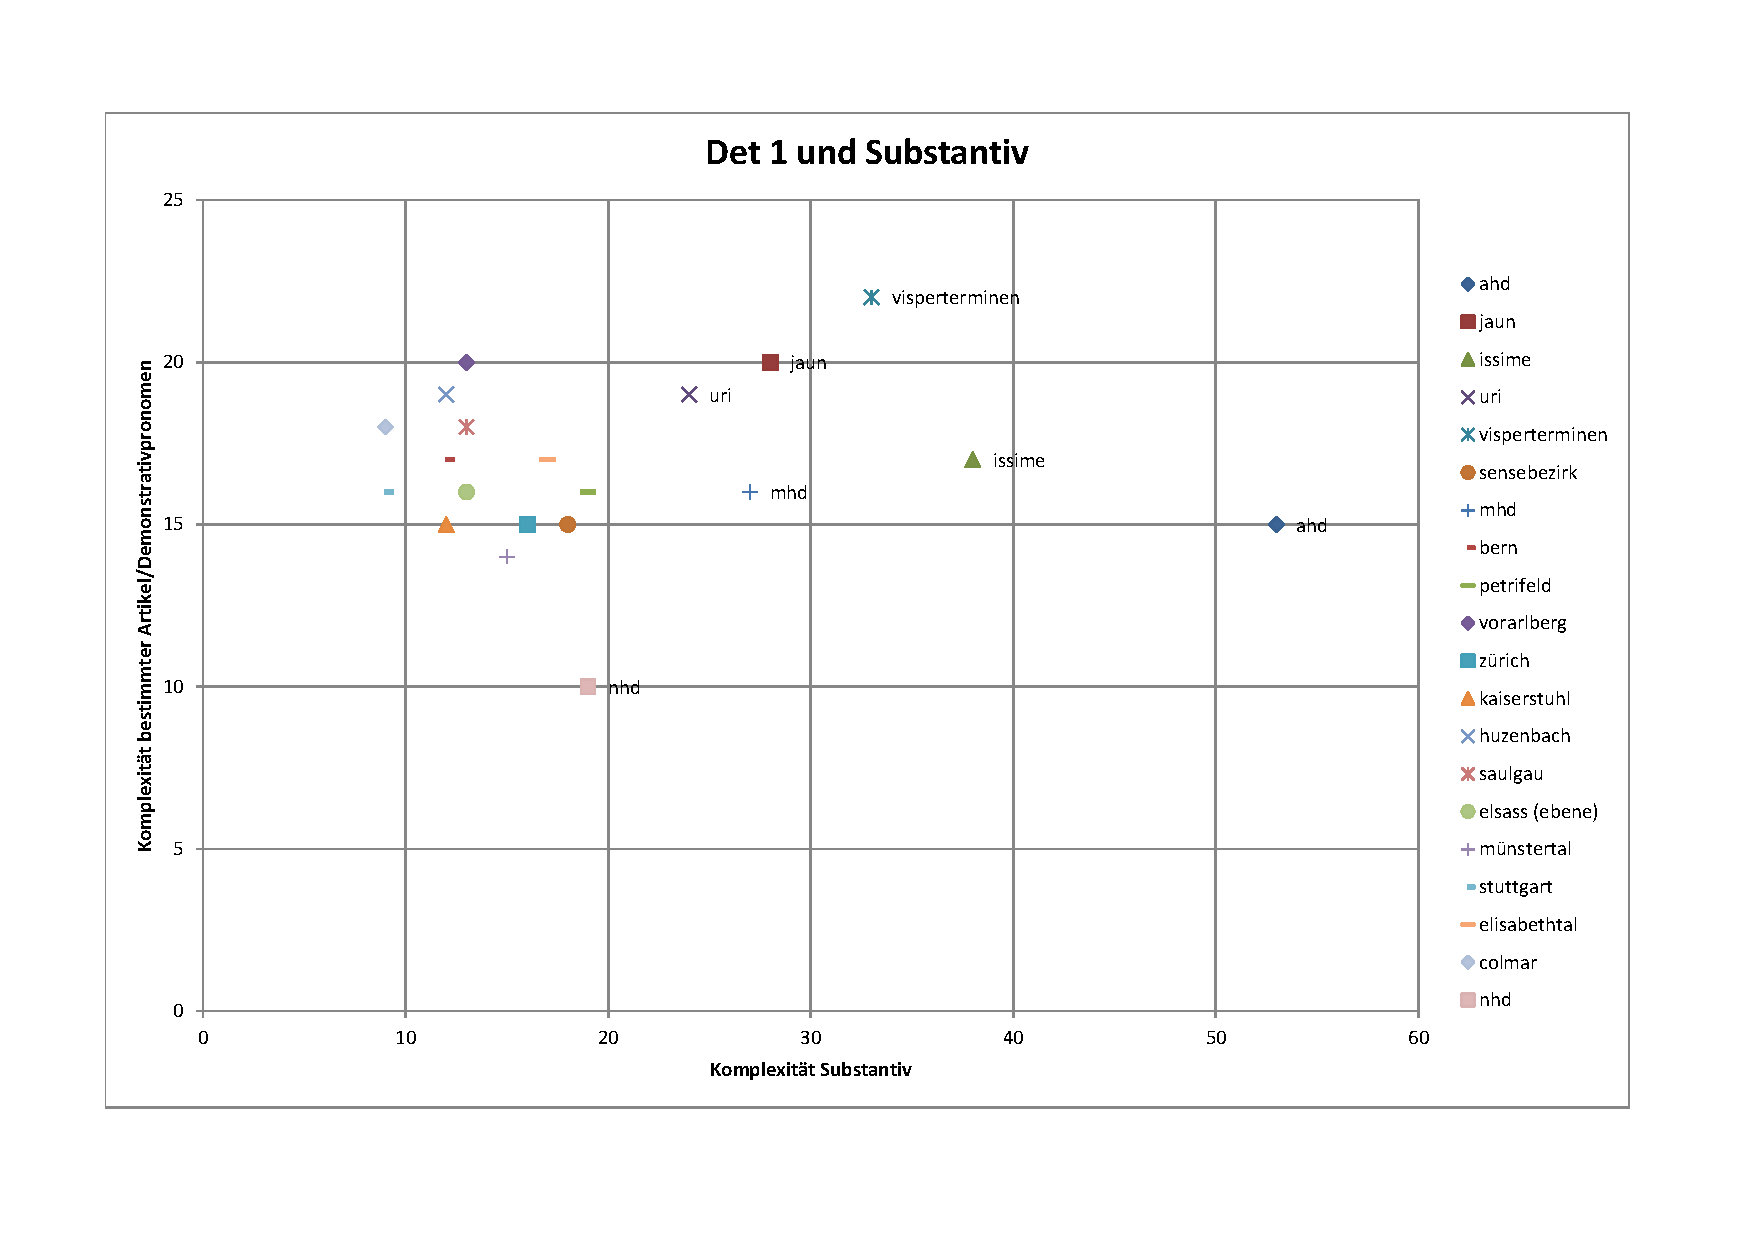
\includegraphics[width=\textwidth]{figures/substDet1.pdf}
    \caption{Komplexität bestimmter Artikel/Demonstrativpronomen + Substantiv}\label{fig:1}
\end{figure}

\begin{figure}
	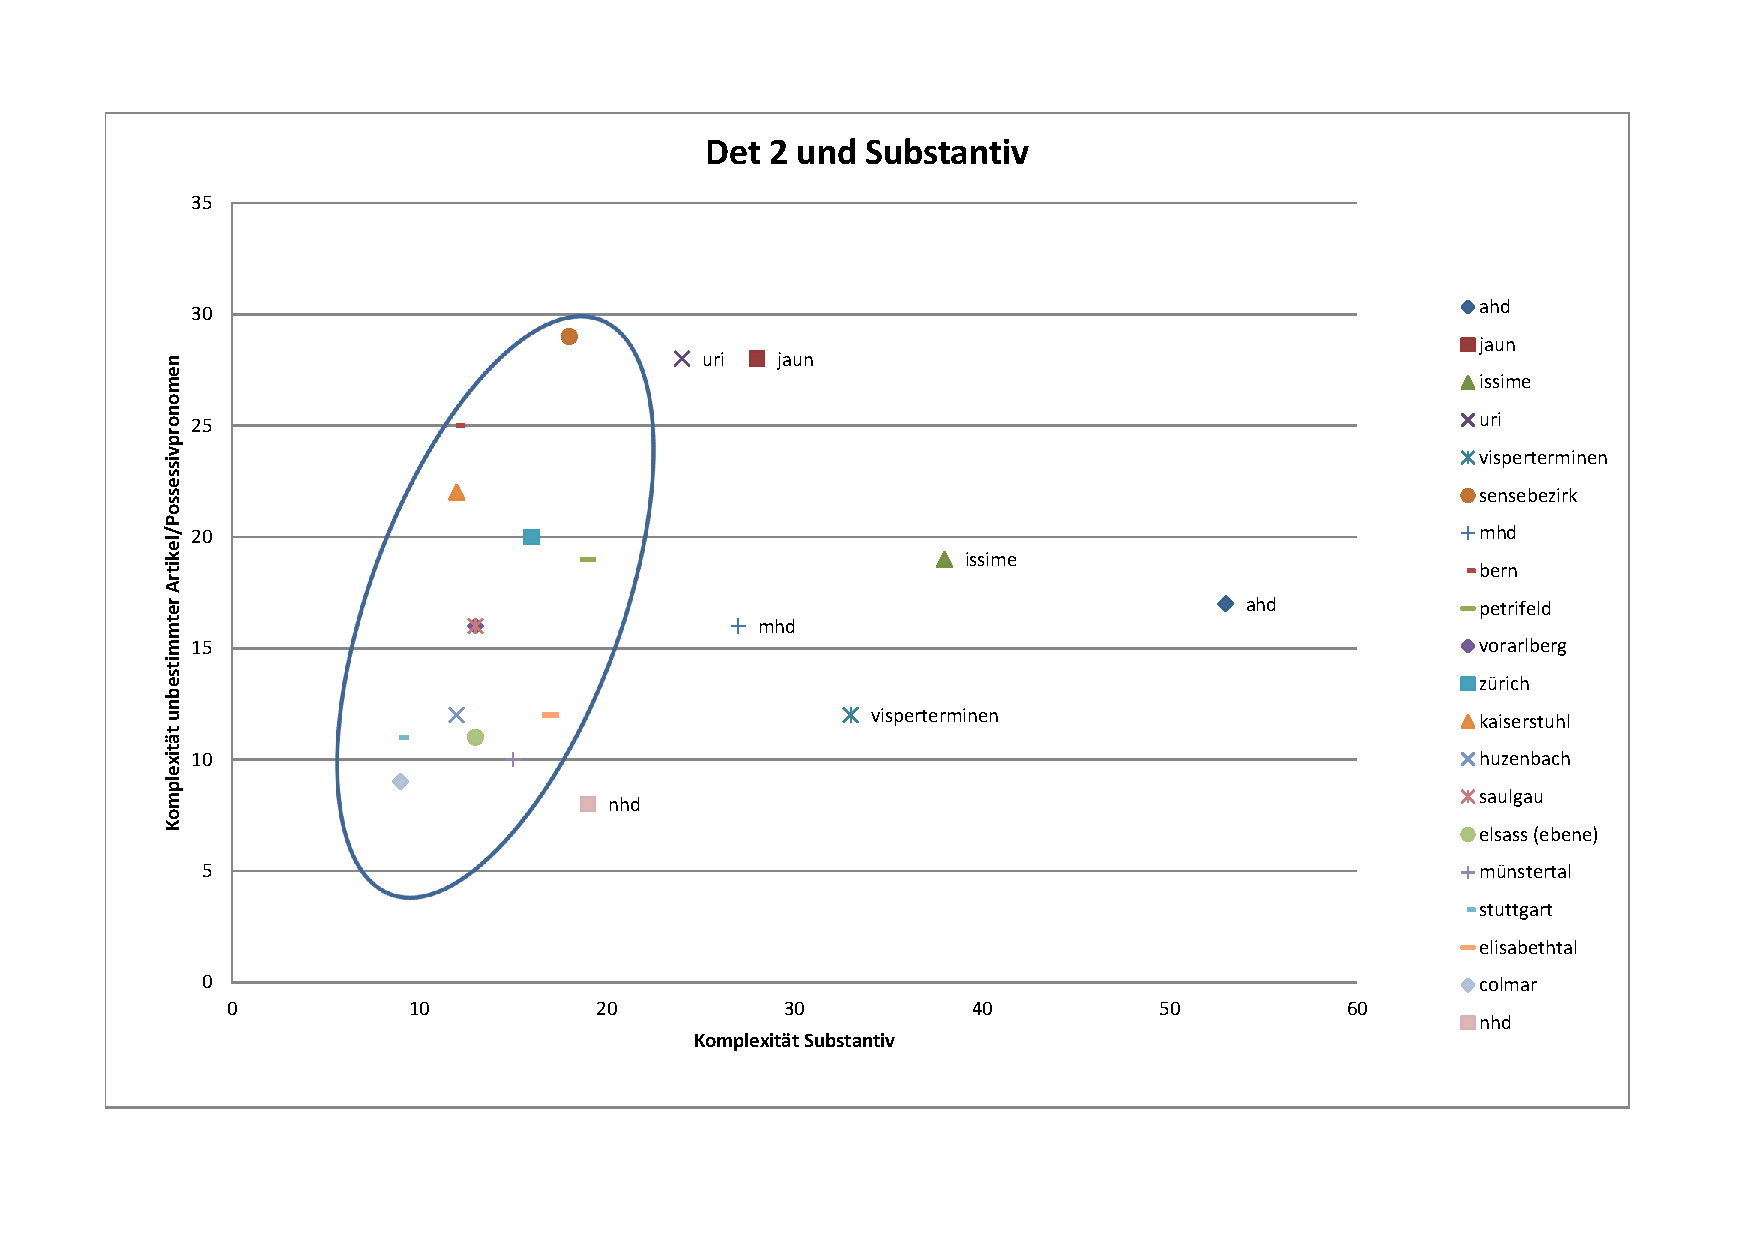
\includegraphics[width=\textwidth]{figures/Det2subst.pdf}
    \caption{Komplexität unbestimmter Artikel / Possessivpronomen + Substantiv}\label{fig:2}
\end{figure}

In \figref{fig:2} ist die Komplexität des Det2 auf der Y-Achse abgebildet, die Komplexität des \isi{Substantivs} auf der X-Achse. Auch hier stellen die Symbole die Varietäten dar. Interessanterweise zeigt \figref{fig:2} ein völlig anderes Bild als \figref{fig:1}, was gegen einen Komplexitätsausgleich zwischen den Determiniererkategorien und dem \isi{Substantiv} spricht. Gäbe es einen Komplexitätsausgleich, würde man wie in \figref{fig:1} erwarten, dass die Varietäten in der Abbildung von oben links nach unten rechts verteilt sind. Möchte man aber in \figref{fig:2} überhaupt eine Tendenz ausmachen, was einigermaßen schwierig ist, da sich die Dialekte verteilen, ist das Gegenteil der Fall: Die Dialekte sind eher von unten links nach oben rechts angeordnet, d.h., dass Varietäten mit einer niedrigeren Komplexität im \isi{Substantiv} auch tendenziell eine niedrigere Komplexität im Det2 aufweisen. Es gibt aber auch einige Parallelen zur \figref{fig:1}. Erstens weist hier die deutsche Standardsprache im Vergleich zu den alemannischen Dialekten ebenfalls eine relativ hohe Komplexität im \isi{Substantiv}, aber geringe Komplexität im Det2 auf. Zweitens haben Jaun und Uri eine vergleichsweise hohe Komplexität im \isi{Substantiv} wie auch im Det2. Anders verhalten sich die Dialekte von Visperterminen und Issime. Beide zeigen eine hohe Komplexität im \isi{Substantiv}, aber eine mittlere (Issime) bzw. eher geringe (Visperterminen) Komplexität im Det2. Folglich finden sich auch bezüglich des Det2 und des \isi{Substantivs} keine Komplexitätsausgleiche.

\subsection{Zusammenfassung}\label{6.1.4}

Zur \isi{Diachronie} lassen sich die wichtigsten Resultate wie folgt zusammenfassen:

\begin{itemize}
\item
Diachrone Simplifizierung wurde in folgenden Kategorien gefunden: Gesamtkomplexität, \isi{Substantive}, \isi{Adjektive} und \isi{Interrogativpronomen}.
\item
Diachrone Komplexifizierung zeigt ungefähr die Hälfte der Dialekte in den folgenden Kategorien: \isi{Personalpronomen}, Det1 und Det2.
\item
Bei den Dialekten, die diachrone Komplexifizierung aufweisen, handelt es sich leicht häufiger um die isolierten ({\textasciitilde}61\%) als um die nicht isolierten Dialekte ({\textasciitilde}47\%). Ein klarerer Zusammenhang konnte jedoch zwischen diachroner Komplexifizierung und einem diatopischen Faktor gefunden werden: Deutlich mehr hoch- (80\%) und höchstalemannische Dialekte ({\textasciitilde}66\%) zeigen diachrone Komplexifizierung als schwäbische ({\textasciitilde}33\%) und oberrheinalemannische Dialekte ({\textasciitilde}17\%).
\end{itemize}

Des Weiteren wurde ein detaillierterer Blick auf die diachronen Mechanismen vorgenommen. Dazu wurde zuerst das Verhältnis zwischen \isi{Archaismen} und \isi{Innovationen} betrachtet, und zwar in den drei Kategorien, die diachrone Komplexifizierung aufweisen. Anschließend wurde dargestellt, dass der Wandel zu einer kooperativen Flexion nicht auf alle Varietäten zutrifft und dass es keinen Komplexitätsausgleich zwischen den Determinierern und den \isi{Substantiven} gibt.

Zum Verhältnis zwischen \isi{Archaismen} und \isi{Innovationen} kann Folgendes festgehalten werden:

\begin{itemize}
\item
Verglichen wurden die Anzahl von \isi{Innovationen} mit dem Kasuserhalt/-abbau in den Kategorien \isi{Personalpronomen}, Det1 und Det2.
\item
Folgende Kombinationen von \isi{Innovationen} und \isi{Archaismen} wurden gefunden (vgl. \tabref{table6.12}): Kasuserhalt + wenig innovativ (Walser Dialekte), Kasuserhalt + sehr innovativ (Jaun), Kasusabbau + (sehr) innovativ (nicht isoliertes Höchstalemannisch, Hochalemannisch), Kasusabbau + wenig innovativ (Oberrheinalemannisch, Schwäbisch).
\item
Dies zeigt, dass es keinen Ausgleich zwischen \isi{Innovationen} und \isi{Archaismen} gibt, d.h. in diesem Fall auch keinen Komplexitätsausgleich.
\item
Welche Dialekte zu welcher Kombination \isi{Innovation}/\isi{Archaismus} gehören, kann nicht aufgrund des Typs der Sprachgemeinschaft, sondern diatopisch bestimmt werden.
\end{itemize}

Schließlich wurde der Wandel zu einer kooperativen Flexion als allgemeines Prinzip für die modernen deutschen Varietäten hinterfragt. Folgendes wurde beobachtet:\largerpage[2]

\begin{itemize}
\item
Alle modernen Varietäten haben einen grammatikalisierten Artikel und eine feste Abfolge in der Nominalphrase.
\item
Die isolierten höchstalemannischen Dialekte haben zusätzlich eine reiche Flexionsmorphologie mit Kasusmarkierung am \isi{Substantiv} erhalten. \isi{Kasus} wird in der Nominalphrase also redundant markiert.
\end{itemize}

\noindent
Daraus kann geschlossen werden, dass:

\begin{itemize}
\item
der grammatikalisierte Artikel und die feste Abfolge in der Nominalphrase auch mit einer reichen Flexionsmorphologie am \isi{Substantiv} vorkommen.
\item
die kooperative Flexion nicht für alle modernen Dialekte gilt. Dabei sei noch darauf hingewiesen, dass jede Varietät in diesem Sample (alt und modern) \isi{Synkretismen} zwischen den Nominalphrasen aufweist.
\end{itemize}

Um zu prüfen, ob es wirklich keinen Ausgleich zwischen den Determinierern und dem \isi{Substantiv} gibt, wurde die Komplexität der \isi{Substantive} jener der Determinierer gegenübergestellt. Zusammenfassend kann Folgendes festgehalten werden (vgl. \figref{fig:1} und \figref{fig:2}):

\begin{itemize}
\item
Die deutsche Standardsprache verhält sich klar anders als die Dialekte. Verallgemeinerungen zu den diachronen Prozessen im Deutschen, die auf dem Vergleich Alt-/Mittelhochdeutsch mit der deutschen Standardsprache basieren, sind also problematisch.
\item
Uri und Jaun: Im \isi{Substantiv} wie auch in den Determiniererkategorien vergleichsweise hohe Komplexität.
\item
Walser Dialekte: Hohe Komplexität im \isi{Substantiv}; Issime mittlere Komplexität im Det1 und Det2; Visperterminen hohe Komplexität im Det1, eher geringe Komplexität im Det2.
\item
Die übrigen Dialekte: Im Det1/\isi{Substantiv} weisen sie gewissen Ähnlichkeiten auf, trotzdem ist die \isi{Variation} zu groß, als dass von einem Komplexitätsausgleich gesprochen werden könnte; Im Det2/\isi{Substantiv} kann beobachtet werden, dass tendenziell Dialekte mit höherer Komplexität am \isi{Substantiv} auch eher höhere Komplexität im Det2 aufweisen.
\end{itemize}

\noindent
Daraus kann geschlossen werden, dass:

\begin{itemize}
\item
die Unterschiede zwischen den Varietäten zu groß sind, als dass ein allgemeines diachrones Prinzip gefunden werden könnte, das für alle modernen Varietäten gilt.
\item
es keinen eindeutigen Komplexitätsausgleich zwischen den Determinierern und den \isi{Substantiven} gibt (Ähnliches wird im folgenden Kapitel gezeigt).
\end{itemize}

\section{Dialektgruppen}\label{6.2}

Im vorangehenden Kapitel konnte gezeigt werden, dass diachrone Komplexifizierung in bestimmten \isi{Dialektgruppen} häufiger vorkommt als in anderen. Berechnet man die durchschnittliche Anzahl der Dialekte pro \isi{Dialektgruppe}, die diachrone Komplexifizierung aufweisen (\tabref{table6.10}), die durchschnittliche Anzahl der diachron komplexifizierten Kategorien pro \isi{Dialektgruppe} (\tabref{table6.11}) sowie die durchschnittliche Anzahl der diachron komplexifizierten Phänomene pro Kategorie und \isi{Dialektgruppe} (\tabref{table6.16}), so wurde immer die gleiche Reihenfolge der \isi{Dialektgruppen} gefunden: Höchstalemannisch > Hochalemannisch > Schwäbisch > Oberrheinalemannisch. Nach diesen diachronen Beobachtungen sollen die \isi{Dialektgruppen} hier synchron verglichen werden, wobei Folgendes im Zentrum steht: Erstens ergibt sich für die \isi{Dialektgruppen} (mit Ausnahme des Schwäbischen) dieselbe Reihenfolge  wie in \sectref{6.1} zur \isi{Diachronie}, betrachtet man die Gesamtkomplexität der einzelnen Dialekte (\tabref{table6.17}). Zweitens gilt dasselbe (mit einzelnen Ausnahmen), wenn man die durchschnittliche Komplexität der einzelnen untersuchten Kategorien und der Gesamtkomplexität pro \isi{Dialektgruppe} berechnet (\tabref{table6.18}). Geschlossen wird das Kapitel mit Überlegungen dazu, was die Resultate für die klassische Einteilung der Dialekte und für die \is{Equi-Complexity-Hypothese}\textit{Equi}{}-\textit{Complexity}{}-Hypothese bedeuten.

\subsection{Beschreibung der Resultate}\label{6.2.1}

\tabref{table6.17} gibt die Gesamtkomplexität (synchron) der untersuchten Dialekte wieder. Daraus wird ersichtlich, dass alle höchstalemannischen Dialekte komplexer sind als alle hochalemannischen und alle hochalemannischen komplexer als alle oberrheinalemannischen. Nur die schwäbischen Dialekte sind verteilt. Petrifeld steht in der hochalemannischen Gruppe, Huzenbach und Saulgau stehen zwischen dem badischen und elsässischen Oberrheinalemannischen und Stuttgart sowie Elisabethtal in der Gruppe des elsässischen Oberrheinalemannischen. Auf den ersten Blick mag dieses sehr klare Ergebnis bezüglich der Reihenfolge von mehr und weniger komplexen \isi{Dialektgruppen} erstaunlich sein. Diese Resultate, also die Komplexität in der nominalen Flexionsmorphologie, bestätigen jedoch die klassische Dialekteinteilung in Höchst-, Hoch- und Niederalemannisch (=Oberrheinalemannisch und Schwäbisch) (mit Ausnahme von Petrifeld, Sprachinsel!).



Um Genaueres zum Schwäbischen im Vergleich zu den anderen \isi{Dialektgruppen} zu erfahren, wurde für jede \isi{Dialektgruppe} das arithmetische Mittel der Komplexität ermittelt. Und zwar wurde dies nicht nur für die Gesamtkomplexität, sondern auch für jede untersuchte Kategorie durchgeführt, um auch diese miteinander vergleichen zu können. Zusammengefasst sind die Resultate in der \tabref{table6.18}.

% % {\tabref{table6.17}: Gesamtkomplexität (\isi{Dialektgruppe})}\\

\begin{table}[]
\caption{Gesamtkomplexität (Dialektgruppe)}\label{table6.17}
\begin{tabular}{llr}
\lsptoprule
% % \multicolumn{3}{l}{{Gesamtkomplexität (alle Kategorien)}}  \\
{DG} & {Varietät} & {Komplexität}\\\midrule
h-st & Jaun & 151\\
h-st & Issime & 141\\
h-st & Uri & 136\\
h-st & Visperterminen & 130\\
h-st & Sensebezirk & 126\\
hoch & Bern & 115\\
schw & Petrifeld & 104\\
hoch & Vorarlberg & 104\\
hoch & Zürich & 103\\
oberr & Kaiserstuhl & 99\\
schw & Huzenbach & 97\\
schw & Saulgau & 95\\
oberr & Elsass (Ebene) & 89\\
oberr & Münstertal & 88\\
schw & Stuttgart & 87\\
schw & Elisabethtal & 87\\
oberr & Colmar & 86\\
\lspbottomrule
\end{tabular}
\end{table}

% % {\tabref{table6.18}: Durchschnittliche Komplexität pro \isi{Dialektgruppe} und Kategorie}\\

\begin{table}[]
\caption{Durchschnittliche Komplexität pro Dialektgruppe und Kategorie}\label{table6.18}
\resizebox{\textwidth}{!}{\begin{tabular}{lS[table-format=2.2]S[table-format=2.2]S[table-format=2.2]S[table-format=2.2]S[table-format=2.2]S[table-format=2.2]S[table-format=2.2]}
\lsptoprule
& \multicolumn{1}{c}{gesamt} & \multicolumn{1}{c}{Det1} & \multicolumn{1}{c}{Det2} & \multicolumn{1}{c}{Pron. inter.} & \multicolumn{1}{c}{Pron. pers.} & \multicolumn{1}{c}{Adj.} & \multicolumn{1}{c}{Nomen}\\\midrule

h-st & 136,2 & 18,6 & 23,2 & 3,8 & 50,4 & 12 & 28,2\\

hoch & 106,67 & 17,34 & 20,34 & 3,67 & 42 & 9,67 & \bfseries 13,67\\

schw & 94 & 17,2 & 14 & \bfseries 5,4 & \bfseries 35,8 & \bfseries 7,6 & \bfseries 14\\

oberr & 90 & 15,75 & 13 & 3,25 & \bfseries 36,5 & \bfseries 9,25 & 12,25\\

\mbox{oberr (Baden)} & 99 & \bfseries 15 & 22 & \bfseries 3 & 37 & 10 & \bfseries 12\\

\mbox{oberr (Elsass)} & 87 & \bfseries 16 & 10 & \bfseries 3,34 & 36,34 & 9 & \bfseries 12,34\\
\lspbottomrule
\end{tabular}}
\end{table}

In der Gesamtkomplexität sind höchstalemannische Dialekte im Durchschnitt komplexer als hochalemannische, hochalemannische komplexer als schwäbische und schwäbische komplexer als oberrheinalemannische. Dasselbe gilt für die Kategorien Det1 sowie Det2. Im \isi{Personalpronomen} und \isi{Adjektiv} bildet Schwäbisch eine Ausnahme, da es weniger komplex als Oberrheinalemannisch ist, wobei der Unterschied besonders im \isi{Personalpronomen} sehr klein ausfällt. Auch im Nomen stellt Schwäbisch eine Ausnahme dar: Es ist komplexer als Hochalemannisch, der Komplexitätsunterschied zwischen diesen beiden \isi{Dialektgruppen} ist aber minimal. Bezüglich des \isi{Interrogativpronomens} wurde bereits in \sectref{6.1.1}) darauf hingewiesen, dass sich die Dialekte in dieser Kategorie nur wenig unterscheiden (vgl. \tabref{table6.2}). Auch hier bildet das Schwäbische eine Ausnahme, weil es komplexer ist als alle anderen \isi{Dialektgruppen}, was vor allem auf die vielen freien Varianten zurückgeführt werden kann (vgl. Paradigmen 72–76). Im Allgemeinen lautet die Komplexitätsreihenfolge folglich Höchstalemannisch > Hochalemannisch > Schwäbisch > Oberrheinalemannisch. Eine Ausnahme hiervon zeigt nur das Schwäbische in einigen Kategorien, jedoch nicht in der Gesamtkomplexität. Die Reihenfolge Höchstalemannisch > Hochalemannisch > Oberrheinalemannisch ist in allen Kategorien und in der Gesamtkomplexität fest.

Es kann hier noch das badische mit dem elsässischen Oberrheinalemannischen verglichen werden (\tabref{table6.18}), auch wenn dieser Vergleich problematisch ist, da das badische Oberrheinalemannisch nur durch einen Dialekt (Kaiserstuhl Alemannisch) vertreten ist. Trotzdem fällt der relativ große Unterschied in der Gesamtkomplexität auf. Dieser kann vorwiegend durch die Resultate der Kategorie Det2 erklärt werden, die ebenfalls einen großen Komplexitätsunterschied zeigt. In allen anderen Kategorien sind die beiden oberrheinalemannischen Untergruppen fast gleich komplex. In der Kategorie Det2 unterscheidet sich das badische vom elsässischen Oberrheinalemannischen vor allem im \isi{Possessivpronomen}: Im Dialekt des Kaiserstuhls (=badisch) verfügt das \isi{Possessivpronomen} über viele freie Varianten im Dativ wie auch über drei unterschiedliche Paradigmen, abhängig von den morphosyntaktischen Eigenschaften des \isi{Possessivpronomens} (vgl. Paradigma 117). Im Gegensatz dazu haben die elsässischen oberrheinalemannischen Dialekte im \isi{Possessivpronomen} keine freien Varianten und nur ein Flexionsparadigma (vgl. Paradigmen 118–120).

\subsection{Analyse und Zusammenfassung}\label{6.2.2}

Aus diesen Ausführungen ergibt sich die folgende Reihenfolge von den komplexeren zu den weniger komplexen \isi{Dialektgruppen}: Höchstalemannisch > Hochalemannisch > Schwäbisch > Oberrheinalemannisch. Nur das Schwäbische weicht in den Kategorien \isi{Personalpronomen}, \isi{Adjektiv} und Nomen davon ab (im \isi{Interrogativpronomen} unterscheiden sich die Dialekte nur sehr wenig). Keine Ausnahmen gibt es bezüglich der Reihenfolge Höchstalemannisch > Hochalemannisch > Oberrheinalemannisch.

Dieses Ergebnis unterstützt klar die traditionelle Einteilung der alemanni-\linebreak schen Dialekte in Höchst-, Hoch- und Oberrheinalemannisch und Schwäbisch.\footnote{Das Bodenseealemannische konnte hier nicht berücksichtigt werden, da für dieses Gebiet keine vollständigen Beschreibungen der Nominalflexion vorhanden sind (vgl. \sectref{3.3.3}).} Diese klassische Einteilung basiert auf phonologischen, morphologischen, syntaktischen und semantischen Isoglossen, die vor allem in den großen Atlasprojekten gefunden wurden. Mit den hier vorgestellten Resultaten kommt ein quantitatives Kriterium aus der Morphologie hinzu: die strukturelle Komplexität der Nominalflexion.

Wichtig sind diese Ergebnisse auch bei der Überprüfung der \is{Equi-Complexity-Hypothese}\textit{Equi}{}-\textit{Complexity}{}-Hypothese. Wären unter dem Strich alle Sprachen/Varietäten gleich komplex, müsste dies nicht nur aus der Gesamtkomplexität, sondern auch aus dem Vergleich der einzelnen Kategorien ersichtlich sein. Wir würden dann bspw. erwarten, dass Dialekt A in der Kategorie X (z.\,B.\ Det1) komplexer als Dialekt B ist, jedoch Dialekt B in der Kategorie Y (z.\,B.\ \isi{Substantiv}) komplexer als Dialekt A. Genau das Gegenteil ist jedoch in den hier vorgestellten Resultaten der Fall: Eine \isi{Dialektgruppe} ist durchschnittlich in jeder Kategorie komplexer als eine andere, die Abfolge von mehr und weniger komplexen \isi{Dialektgruppen} ist in jeder Kategorie dieselbe (mit den genannten Ausnahmen im Schwäbischen). Gewisse \isi{Dialektgruppen} markieren folglich die morphosyntaktischen Eigenschaften innerhalb der Nominalphrase deutlich redundanter als andere \isi{Dialektgruppen}. Ergebnisse, die in dieselbe Richtung gehen, wurden in \sectref{6.1.3} bezüglich der Determinierer und \isi{Substantive} der einzelnen Dialekte gezeigt. Diese Resultate beziehen sich natürlich ausschließlich auf die nominale Flexionsmorphologie. Es kann also hier nicht ausgeschlossen werden, dass der Abbau in der Flexionsmorphologie nicht doch z.\,B.\ in der Syntax ausgeglichen wird. An die vorliegende Arbeit würde sich also eine umfangreiche vergleichende Studie anbieten, die z.\,B.\ die Markierung von Subjekt und direktem Objekt in den unterschiedlichen alemannischen Dialekten untersucht, z.\,B.\ auf eine ähnliche Art und Weise wie \citet{Sinnemäki2008}. Erste exemplarische Arbeiten existieren bereits, wie z.\,B.\ \citet{Ellsäßer2015}.

In der Komplexität der Nominalflexion der hier untersuchten \isi{Dialektgruppen} und Kategorien konnten also keine Ausgleichstendenzen gefunden werden. Das strikte Gegenteil trifft zu. Natürlich können aus diesen Beobachtungen keine allgemeinen Aussagen abgeleitet werden, die für alle Sprache gelten. Dafür bräuchte es ein viel größeres Sample, in dem alle Sprachfamilien adäquat repräsentiert sind. Es sind mir jedoch auch keine Studien bekannt, die das Gegenteil der Resultate dieser Arbeit nachweisen würden bzw. die überhaupt Ausgleichstendenzen zwischen unterschiedlichen Kategorien der Nominalflexion prüfen.

\section{Kontakt}\label{6.3}

Wie in \sectref{2.2.3} dargestellt wurde, kann intensiver \isi{Sprachkontakt} sowohl zu höherer als auch zu niedrigerer Komplexität führen, und zwar abhängig vom Typ der Sprachgemeinschaft. Höhere Komplexität wird in einer sehr langen koterritorialen Kontaktsituation erwartet, in der Kinder zwei- oder mehrsprachig aufwachsen \citep[34]{Trudgill2011}. In Sprachen solcher Sprachgemeinschaften sind \textit{Additive Borrowings} zu beobachten, also Elemente oder Kategorien, die von der einen Sprache in die andere übernommen werden, ohne dass jedoch in der übernehmenden Sprache schon vorhandene Elemente oder Kategorien ersetzt werden \citep[27]{Trudgill2011}. Aus dem untersuchten Sample passen die Sprachinseln Elisabethtal, Petrifeld und Issime sowie die elsässischen Dialekte zu diesem Typ von Sprachgemeinschaft (vgl. Beschreibung der Sprachgemeinschaften dieser Dialekte in \sectref{3.3.3}). Im Gegensatz dazu weisen große Sprachgemeinschaften mit vielen Kontakten, losen Netzwerken und vielen L2-Ler\-nern Simplifizierungen auf \citep[146–147]{Trudgill2011}. In \sectref{3.2.3} wurde argumentiert, dass zur Überprüfung dieser Hypothese Stadt- mit Landdialekten verglichen werden können. Die Stadtdialekte in diesem Sample sind Bern, Zürich (beide Hochalemannisch), Colmar (Oberrheinalemannisch) und Stuttgart (Schwäbisch). Aus dem höchstalemannischen Gebiet gibt es keine vollständige Beschreibung der nominalen Flexionsmorphologie eines Stadtdialekts. Auch die deutsche Standardsprache entspricht jener Sprachgemeinschaft, in der Simplifizierung erwartet wird. Sie wird in \sectref{6.3} gesondert behandelt. Zuerst werden nun die Sprachinseln sowie die elsässischen Dialekte betrachtet und anschließend die Stadt- mit den Landdialekten verglichen.

\subsection{Sprachinseln und Elsass}\label{6.3.1}

In den Sprachinseln Issime, Petrifeld und Elisabethtal sowie in den elsässischen Dialekten sind also \textit{Additive Borrowings} zu erwarten. Interessanterweise wurde aber nur ein \textit{Additive Borrowing} gefunden, und zwar im \isi{Personalpronomen} im Plural des Dialekts von Issime (ausführlich vorgestellt in \sectref{5.3.1}). Zwar weisen Petrifeld, Elisabethtal und die elsässischen Dialekte Lehnwörter aus den jeweiligen Kontaktsprachen auf, diese sind jedoch in das phonologische und morphologische System der alemannischen Dialekte integriert (\citealt[54]{Beyer1963}, \citealt[102–103]{Moser1937}, \citealt[52]{Žirmunskij1928/29}).

Es stellt sich nun die Frage, was Issime von den anderen Sprachinseln und den elsässischen Dialekten unterscheidet. Erstens ist Issime eine deutlich ältere Sprachinsel (seit dem 13. Jh.) als Petrifeld (seit Mitte des 18. Jhs.) und Elisabethtal (seit Anfang des 19. Jhs.). Auch im Elsass breitete sich die deutsch-französische Zweisprachigkeit erst seit der Französischen Revolution allmählich aus (ausführlich in \sectref{3.3.3}). Zweitens setzt ein \textit{Additive Borrowing} voraus, dass die Sprecher bereits als Kinder in beiden Sprachen eine hohe Kompetenz erworben haben, was auf die Alemannischsprecher in Issime zutrifft (vgl. \sectref{3.3.3}). Keine Angaben zur Kompetenz in den Kontaktsprachen, die die Alemannischsprecher von Petrifeld und Elisabethtal hatten (zum Zeitpunkt der Publikation der \isi{Ortsgrammatiken}), konnten gefunden werden. Im Elsass dehnte sich der Bilingualismus erst nach der Französischen Revolution langsam aus, in weiten Bevölkerungsteilen aber erst seit dem Ende des 2. Weltkriegs durch die obligatorische Schule auf Französisch (abgesehen von jenen Sprechern, die einen Sprachwechsel vollzogen haben) (vgl. \sectref{3.3.3}). Im Gegensatz zu den beiden anderen Sprachinseln und den elsässischen Dialekten ist in Issime Mehrsprachigkeit bereits bei Kindern nicht nur gesichert nachweisbar, sondern (im Gegensatz zu den elsässischen Dialekten) seit jeher vorhanden.

Der Dialekt bzw. die Sprachgemeinschaft von Issime bringt also sozusagen die optimalen Voraussetzungen für ein \textit{Additive Borrowing} mit. Es ist jedoch bemerkenswert, dass auch in diesem optimalen Kontext nur ein \textit{Additive Borrowing} vorhanden ist. Zu überlegen ist folglich, ob die \textit{Additive Borrowings} nicht allgemein ein eher seltenes Phänomen darstellen. Das heißt ebenfalls, wie zu erwarten ist, dass die Flexionsmorphologie in Kontaktsituationen deutlich stabiler bleibt als das Lexikon. Dies ist auch daran ersichtlich, dass Petrifeld, Elisabethtal und die elsässischen Dialekte sehr wohl entlehnte Lexeme aus den Kontaktsprachen aufweisen. Andere Studien zeigen jedoch, dass \textit{Additive Borrowings} in bestimmten Kontaktsituationen durchaus üblich sind (vgl. z.\,B.\ \citealt{King2000}). Bezogen auf Issime und auf die Nominalflexion ist jedoch auch zu beachten, dass die Kontaktsprachen nicht viele Möglichkeiten für komplexitätsaufbauende \textit{Additive Borrowings} bieten, da die Kontaktsprachen im Vergleich zu Issime Alemannisch eine eher arme nominale Flexionsmorphologie aufweisen. Was die Kontaktsprachen in der Nominalflexion markieren, markiert Issime sowieso schon (mit der ursprünglichen Ausnahme der Doppelformen im Plural des \isi{Personalpronomens}). Dem Phänomen der \textit{Additive Borrowings} sollte also gesondert genauer nachgegangen werden. Dabei sollte sprachvergleichend vorgegangen werden, aber auch unterschiedliche soziolinguistische Kontexten sollten berücksichtigt werden. Des Weiteren wären auch \textit{Additive Borrowings} auf allen linguistischen Beschreibungsebenen einzubeziehen.

\subsection{Stadtdialekte vs. Landdialekte}\label{6.3.2}

In \sectref{6.2} wurde gezeigt, dass die verschiedenen alemannischen \isi{Dialektgruppen} sich klar in ihrer Komplexität unterscheiden. Deswegen werden hier die Stadt- mit den Landdialekten jeweils innerhalb derselben \isi{Dialektgruppe} verglichen.

Die Resultate des Vergleichs der schwäbischen und oberrheinalemannischen Stadt- und Landdialekte sind in \tabref{table6.19} zusammengefasst, die auf den Resultaten der Tabellen \ref{table6.1}–\ref{table6.3} und \ref{table6.5}–\ref{table6.8} basieren. Das Symbol \ding{52} steht, wenn der Stadtdialekt weniger komplex ist als alle Landdialekte, das Symbol (\ding{52}), wenn der Stadtdialekt und ein Landdialekt dieselbe Komplexität aufweisen und beide weniger komplex sind als alle Landdialekte, das Symbol \ding{55}, wenn der Stadtdialekt nicht weniger komplex ist als alle Landdialekte. Aus der \tabref{table6.19} ist ersichtlich, dass in fünf von sechs Kategorien und in der Gesamtkomplexität der Stadtdialekt weniger komplex ist als die Landdialekte (mit einem Landdialekt derselben Komplexität in einigen Kategorien). Im \isi{Personalpronomen} trifft dies nur auf Colmar zu, im Det1 nur auf Stuttgart und im \isi{Adjektiv} auf keine der beiden Städte. Wir können also festhalten, dass es in den \isi{Dialektgruppen} Oberrheinalemannisch und Schwäbisch zumindest eine Tendenz dazu gibt, dass Stadtdialekte weniger komplex sind als Landdialekte. Dies entspricht \citeauthor{Trudgill2011}s \citeyearpar{Trudgill2011} Annahmen über die Komplexität von Sprachen, die von Sprachgemeinschaften mit vielen Kontakten, losen Netzwerken und vielen L2-Ler\-nern gesprochen werden.

Des Weiteren zeigen sich erstaunliche Parallelen zwischen Schwäbisch und Oberrheinalemannisch. Erstens unterscheiden sich die Resultate dieser \isi{Dialektgruppen} nicht, da generell die Stadtdialekte weniger komplex sind als alle Landdialekte. Eine Ausnahme hiervon bilden nur die Kategorien \isi{Personalpronomen} und Det1 (\tabref{table6.19}). Zweitens sind die Stadtdialekte in den Kategorien \isi{Adjektiv} und Det1 (nur Colmar) komplexer als alle Landdialekte (Tabellen \ref{table6.3} und \ref{table6.8}), im \isi{Personalpronomen} liegt Stuttgart auf dem dritten Platz (von fünf) (\tabref{table6.6}).

% % {\tabref{table6.19}: Stadtdialekt mit geringster Komplexität im Vergleich mit Landdialekten (Schwäbisch und Oberrheinalemannisch)}\\

\begin{table}
\caption{Stadtdialekt mit geringster Komplexität im Vergleich mit Landdialekten (Schwäbisch und Oberrheinalemannisch)}\label{table6.19}
\begin{tabularx}{\textwidth}{lccccccc}
\lsptoprule
& gesamt & Nomen & Det2 & Pron. inter. & Pron. pers. & Det1 & Adj.\\
\midrule
schw & \ding{52} & \ding{52} & \ding{52} & (\ding{52}) & \ding{55} & (\ding{52}) & \ding{55}\\
oberr & \ding{52} & \ding{52} & \ding{52} & (\ding{52}) & (\ding{52}) & \ding{55} & \ding{55}\\
\lspbottomrule
\end{tabularx}
\end{table}

Ganz andere Resultate sind im Hochalemannischen (\tabref{table6.20}) zu beobachten. Hier sind die beiden Stadtdialekte (Bern und Zürich) nur im Det1 und \isi{Adjektiv} weniger komplex als der Dialekt von Vorarlberg. In den meisten Kategorien und in der Gesamtkomplexität steht Vorarlberg zwischen den beiden Stadtdialekten, wobei Bern in mehr Kategorien als Zürich komplexer ist als Vorarlberg. In der Kategorie Det2 zeigt der Dialekt von Vorarlberg sogar die geringste Komplexität verglichen mit den Stadtdialekten. Eine Tendenz wie in den oberrheinalemannischen und schwäbischen Dialekten mit Stadtdialekten von geringerer Komplexität als Landdialekte ergibt sich aus den hier untersuchten hochalemannischen Dialekten nicht. Außerdem gibt es auch bezüglich der Kategorien keine Parallelen zu den oberrheinalemannischen und schwäbischen Dialekten. Eher das Gegenteil trifft zu: Während die oberrheinalemannischen und schwäbischen Stadtdialekte in den Kategorien \isi{Adjektiv} und Det1 (nur Colmar) höhere Komplexität aufweisen als die Landdialekte (\tabref{table6.19}), zeigt Vorarlberg genau in diesen Kategorien eine höhere Komplexität als die Stadtdialekte (\tabref{table6.20}). Ein weiteres Beispiel ist die Kategorie Det2: Die oberrheinalemannischen und schwäbischen Stadtdialekte haben die geringste Komplexität (\tabref{table6.19}), die hochalemannischen Stadtdialekte jedoch die höchste Komplexität (\tabref{table6.20}).

% % {\tabref{table6.20}: Stadt- und Landdialekte im Hochalemannischen}\\

\begin{table}
\caption{Stadt- und Landdialekte im Hochalemannischen}\label{table6.20}
\begin{tabular}{ll}
\lsptoprule
{Reihenfolge Dialekt}
{(mehr – weniger komplex)} & {Kategorie}\\
\midrule
Vorarlberg – Bern – Zürich & Det1\\
& \isi{Adjektiv}\\
\tablevspace
Bern – Vorarlberg – Zürich & Gesamtkomplexität\\
& \isi{Personalpronomen}\\
\tablevspace
& \isi{Interrogativpronomen}\\
Zürich – Vorarlberg – Bern & Nomen\\
\tablevspace
Bern – Zürich – Vorarlberg & Det2\\
\lspbottomrule
\end{tabular}
\end{table}

Für die Hypothese, dass Stadtdialekte eine geringere Komplexität als Landdialekte aufweisen, konnte in den schwäbischen und oberrheinalemannischen Gruppen eine klare Tendenz gefunden werden. Dies gilt jedoch nicht für die hochalemannischen Dialekte. Des Weiteren konnte gezeigt werden, dass sich die schwäbischen und oberrheinalemannischen Stadt- und Landdialekte in den verschiedenen Kategorien sehr ähnlich verhalten. Auch diesbezüglich weicht das Hochalemannische klar vom Schwäbischen und Oberrheinalemannischen ab.

Eine mögliche Erklärung dafür, dass die hochalemannischen Stadtdialekte abweichen, kann im soziolinguistischen Kontext gefunden werden. Dies soll kurz anhand des Vergleichs der hochalemannischen (= Schweizer) Stadtdialekte mit dem schwäbischen (= deutschen) Stadtdialekt veranschaulicht werden. Wenn in Deutschland Sprecher unterschiedlicher Dialekte miteinander kommunizieren, geschieht dies für gewöhnlich in der Standardsprache. Es wird also auf eine dritte Sprache, auf eine Lingua Franca ausgewichen. Folglich ist zu erwarten, dass in den Stadtdialekten viele standardnahe Formen auftreten, sodass Städte und Ballungsgebiete eine Art Insel darstellen. Dies konnte \citet{Pröll2015} für das Untersuchungsgebiet des Sprachatlas von Bayerisch-Schwaben mithilfe geostatistischer Methoden nachweisen: „Sehr deutlich treten die bevölkerungsreichen Orte als eigene, räumlich diskontinuierliche Struktur hervor […]. Wie zu erwarten war, handelt es sich bei den Phänomenen, die diese „städtische“ Tendenz ausmachen, um standardnähere Formen“ (\citealt[160]{Pröll2015}; vgl. auch Faktor 10 in \citealt[146-147]{Pröll2015}). Des Weiteren strahlen Stadtsprachen auf ihre Umgebung aus, was u.a. durch eine hohe Anzahl von Berufspendlern sowie durch ein höheres Prestige der Stadtdialekte im Gegensatz zu den Landdialekten erklärt werden kann. Davon unterscheidet sich die Situation in der Schweiz grundsätzlich. Wenn Sprecher unterschiedlicher Dialekte miteinander kommunizieren, weichen diese nicht auf eine Lingua Franca aus, sondern jeder Beteiligte verwendet seinen eigenen Dialekt, wobei die gegenseitige Verständlichkeit gewährleistet ist. Vermieden werden eventuell besonders kleinräumige Lexeme, die durch großräumigere Lexeme ersetzt werden. Folglich bilden Städte in der Schweiz keine sprachlichen Inseln, die ein höheres Prestige haben oder auf ihre Umgebung ausstrahlen. Auch dies kann durch erste geostatistische Auswertungen des Materials des Sprachatlas der deutschen Schweiz (SDS) und des Syntaktischen Atlas der deutschen Schweiz (SADS) gezeigt werden (Pröll \& Stöckle: in Vorbereitung).\footnote{Ich danke Simon Pröll für die aufschlussreiche Diskussion zu den Unterschieden zwischen den Städten und für den großzügigen Einblick, den er mir ein seine noch unveröffentlichten Daten und Auswertungen gewährt hat.} Um also Genaueres zur eventuellen Rolle der Schweizer Städte zu erfahren, sollten diese mit Landdialekten desselben Dialektgebiets verglichen werden. Dabei sollten Resultate aus geostatistischen Auswertungen als Grundlage zur Bestimmung der Dialektgebiete dienen.

\section{Standardvarietät}\label{6.4}

Für die Hypothese, dass Sprachen von großen Sprachgemeinschaften mit vielen Kontakten, losen Netzwerken und vielen L2-Ler\-nern eher geringere strukturelle Komplexität aufweisen, konnte im vorangehenden Kapitel für das Schwäbische und Oberrheinalemannische eine Tendenz gefunden werden. Dieser Typ Sprachgemeinschaft passt jedoch noch besser zu einer Standardsprache als zu einem Stadtdialekt. Stadtdialekte sind regional gebunden, was vor allem auf die geschriebene deutsche Standardsprache nur in äußerst geringem Maße zutrifft. Die deutsche Standardsprache wird in verschiedenen Ländern verwendet und ist jene Varietät, die besonders im gesteuerten L2-Er\-werb vermittelt wird. Außerdem wird sie von Deutsch-Muttersprachlern mit einem Dialekt als L1 parallel zum Dialekt oder nach dessen Erwerb gelernt (aufgeführt in \sectref{3.2.4}). Schließlich ist das Ziel einer Standardisierung die Vereinheitlichung, woraus eine Vereinfachung resultieren kann. Gleichzeitig kann jedoch die Kodifizierung einer Sprache dazu führen, dass Elemente der Sprache konserviert werden, d.h., auch \isi{Archaismen} mit höherer Komplexität können erhalten werden. Es stellt sich hier folglich die Frage, welche Kraft stärker ist, ob die nominale Flexionsmorphologie der deutschen Standardsprache mehr oder weniger komplex als die untersuchten alemannischen Dialekte ist.

\subsection{Resultate}\label{6.4.1}

In der Gesamtkomplexität ist die deutsche Standardsprache weniger komplex als alle untersuchten Dialekte (\tabref{table6.1}). Dasselbe gilt für die Kategorien Det1, Det2 und das \isi{Personalpronomen} (Tabellen \ref{table6.6}–\ref{table6.8}). Das standarddeutsche \isi{Substantiv} steht in seiner Komplexität im oberen Mittelfeld (\tabref{table6.5}): Mit einem Grad an Komplexität von 19 liegt es leicht über dem arithmetischen Mittel (\={x}=17,78) und am Anfang des oberen Terzils. Dasselbe trifft auf die Anzahl von \isi{Realisierungsregeln} (9) und \isi{Flexionsklassen} (10) zu (\tabref{table6.4}) (\isi{Realisierungsregeln}: \={x}=8,45; \isi{Flexionsklassen} \={x}=9,34). Die Komplexität des \isi{Interrogativpronomens} ist vergleichsweise hoch, wie jedoch bereits erwähnt wurde, unterscheiden sich die untersuchten Varietäten in der Komplexität des \isi{Interrogativpronomens} nur sehr wenig (\tabref{table6.2}). Eine hohe Komplexität weist das  standarddeutsche \isi{Adjektiv} auf (\tabref{table6.3}). Interessanterweise war dies schon bei den oberrheinalemannischen und schwäbischen Stadtdialekten der Fall, jedoch nicht bei den hochalemannischen Stadtvarietäten (vgl. \sectref{6.3}).

\subsection{Analyse}\label{6.4.2}

Es soll nun überlegt werden, wie diese Resultate erklärt werden können und was diese bezüglich der Komplexifizierung und Simplifizierung einer Standardsprache bedeuten. Dazu wird in der Folge jede Kategorie (exklusive \isi{Interrogativpronomen}) einzeln diskutiert.

Wie schon in \sectref{5.5.3} und \sectref{5.6.2} dargestellt wurde, sind die Wortarten der Kategorien {Det1 und Det2} in der Standardsprache weniger weit grammatikalisiert als in den Dialekten. Die Paradigmen des \isi{Demonstrativpronomens} und des \isi{bestimmten Artikels} einerseits (=Det1) und des \isi{Possessivpronomens} und des \isi{unbestimmten Artikels} andererseits (=Det2) unterscheiden sich im Gegensatz zu den dialektalen Paradigmen nicht (vgl. \sectref{5.5.3} und \sectref{5.6.2}). Zur Definition der Paradigmen der Standardsprache ist also nur ein Satz an \isi{Realisierungsregeln} pro Kategorie nötig, während es in den Dialekten pro Kategorie zwei sind. Dass das \isi{Possessivpronomen} einen Plural hat, der \isi{unbestimmte Artikel} jedoch nicht, fällt nicht ins Gewicht, da bei den \isi{Realisierungsregeln} für den Plural die Wortart spezifiziert ist, bei den \isi{Realisierungsregeln} für den Singular jedoch nicht; die Wortart bleibt unterspezifiziert. Des Weiteren weisen die Dialekte unterschiedliche \isi{Innovationen} in den Kategorien Det1 und Det2 auf, die zu höherer Komplexität führen: syntaktisch bedingte Allomorphie (\sectref{5.5.5} und \sectref{5.6.4}), Possessiv-Artikel (\sectref{5.5.2}), unterschiedliche Paradigmen je nach \isi{Possessivpronomen} (\sectref{5.6.6}), Stammalternationen im \isi{Possessivpronomen} (\sectref{5.6.8}) (vgl. \sectref{6.1.3}). Die deutsche Standardsprache weist keine \isi{Innovationen} auf, aus denen eine höhere Komplexität resultiert.

Im {Personalpronomen} unterscheidet die deutsche Standardsprache betonte und unbetonte \isi{Personalpronomen} in der Flexion nicht. Da im Mittel- und Althochdeutschen in der 3. Person betonte und unbetonte \isi{Personalpronomen} verschiedene Formen aufweisen, kann das Fehlen dieser Unterscheidung als diachrone Simplifizierung interpretiert werden. Alle untersuchten Dialekte jedoch haben diese Unterscheidung ausgebaut und verfügen heute über ein vollständiges Paradigma an betonten Formen und über eines an unbetonten Formen (vgl. \sectref{5.3.2} und \sectref{6.1.3}). Einige alemannische Dialekte unterscheiden zusätzlich in der 3. Person Singular Neutrum eine belebte von einer unbelebten Form (vgl. \sectref{5.3.3} und \sectref{6.1.3}). Es handelt sich dabei um eine \isi{Innovation}, die zu höherer Komplexität führt. Wie im Det1 und Det2 weist die deutsche Standardsprache auch im \isi{Personalpronomen} keine solchen \isi{Innovationen} auf.

Im Vergleich zu den alemannischen Dialekten zeigt die deutsche Standardsprache im {Adjektiv} eine hohe Komplexität. Dies ist erstens durch den Erhalt des Genitivs zu erklären, dessen Formen durch \isi{Realisierungsregeln} definiert werden müssen. Mit Ausnahme der isolierten höchstalemannischen Dialekte gibt es in der Adjektivflexion der alemannischen Dialekte keinen Genitiv mehr. Zweitens hat jede Zelle des standardsprachlichen Adjektivparadigmas ein \isi{Suffix}, das durch \isi{Realisierungsregeln} definiert werden muss. Im Gegensatz dazu sind Zellen ohne Endung ein häufiges Phänomen in den alemannischen Dialekten (vgl. Paradigmen 24–40), für die auch keine \isi{Realisierungsregeln} nötig sind, was folglich zu einer niedrigeren Komplexität führt. Zwar konnten \isi{Adjektive} auch im Alt- und Mittelhochdeutschen unflektiert bleiben (= nominale Formen). Allerdings standen diese unflektierten Adjketive mit flektierten \isi{Adjektiven} in derselbe Zelle des Paradigmas in \isi{Variation}. Der Erhalt des Genitivs kann folglich als Konservierung verstanden werden (d.h. hier Erhalt von Komplexität), das Fehlen von unflektierten attributiven \isi{Adjektiven} als Neuerung (d.h. hier Aufbau von Komplexität).

Auch die Komplexität des standardsprachlichen {Substantivs} ist vergleichsweise hoch. Generell wird für die deutsche Standardsprache von einem vier-Kasus-System ausgegangen. Zählt man aber, wie viele \isi{Kasus} maximal pro \isi{Flexionsklasse} markiert werden, so kommt man auf zwei \isi{Kasus} (vgl. \sectref{6.1.3}). Die alemannischen Dialekte jedoch markieren generell am \isi{Substantiv} überhaupt keine \isi{Kasus}.\footnote{Mit wenigen Ausnahmen in Uri (Paradigma 8), Vorarlberg (Paradigma 9), Zürich (Paradigma 10), Petrifeld (Paradigma 15) und Elisabethtal (Paradigma 16).} Eine Ausnahme bilden hier nur die drei isolierten höchstalemannischen Dialekte, die höchstens drei \isi{Kasus} pro \isi{Flexionsklasse} markieren (vgl. \sectref{6.1.3}). Wie in der Adjektivflexion hat die deutsche Standardsprache also auch in der Substantivflexion \isi{Archaismen} bewahrt, die die strukturelle Komplexität erhöhen.

Es ist noch zu klären, ob eventuell eine weitere Ursache für die hohe Komplexität im standarddeutschen \isi{Substantiv} in der Pluralmarkierung liegt. Dazu wurde gezählt, wie viele unterschiedliche Pluralmarker jede moderne Varietät dieses Samples hat. Dabei ist noch zu erwähnen, dass die Nominativ-Plural-Endung genommen wurde, wenn \isi{Numerus} und \isi{Kasus} kumulativ markiert werden, wie z.\,B.\ in Issime: \textit{weg}–\textit{a} (Nominativ/Akkusativ Plural), \textit{weg}–\textit{e} (Dativ Plural), \textit{weg}–\textit{u} (Genitiv Plural) (Zürrer 1999: 164, Paradigma 4). Neben dem Dialekt von Issime kommt dies auch in den Dialekten von Visperterminen, Jaun und Uri vor. Die Resultate sind in der \tabref{table6.21} zusammengefasst. Es zeigt sich, dass die deutsche Standardsprache über eine durchschnittliche Anzahl Pluralmarker verfügt, folglich steht die hohe Komplexität in der standardsprachlichen Substantivflexion nicht mit der Pluralmarkierung in Zusammenhang.

% % {\tabref{table6.21}: Anzahl Pluralmarker pro moderne Varietät}\\

\begin{table}
\caption{Anzahl Pluralmarker pro moderne Varietät}\label{table6.21}
\begin{tabularx}{\textwidth}{cX}
\lsptoprule
{Anzahl Pluralmarker} & {Varietäten}\\
\midrule
3 & Vorarlberg\\
% % \midrule
4 & Bern, Stuttgart, Colmar \\
% % \midrule
5 & Zürich, Huzenbach, Saulgau, Elisabethtal, Kaiserstuhl, Elsass (Ebene), deutsche Standardsprache\\
% % \midrule
6 & Münstertal\\
% % \midrule
7 & Issime, Jaun, Sensebezirk, Petrifeld\\
% % \midrule
8 & Visperterminen, Uri\\
\lspbottomrule
\end{tabularx}
\end{table}

{Zusammengefasst} können wir also Folgendes festhalten: Die deutsche Standardsprache zeigt eine relativ hohe Komplexität in der Adjektiv- und Substantivflexion, was vor allem auf den Erhalt von solchen \isi{Archaismen} zurückzuführen ist, die höhere Komplexität verursachen (z.\,B.\ Kasuserhalt). Gleichzeitig hat die deutsche Standardsprache die niedrigste Komplexität in der Flexion der Kategorien Det1, Det2 und \isi{Personalpronomen}. Zwar hat sie hier im Gegensatz zu den meisten alemannischen Dialekten den Genitiv erhalten. Die alemannischen Dialekte zeigen aber in diesen drei Kategorien zahlreiche \isi{Innovationen}, die zu einem Zuwachs an Komplexität geführt haben. Die deutsche Standardsprache weist keine dieser \isi{Innovationen} auf. Sie kodiert also deutlich weniger Unterscheidungen in der Flexion als die alemannischen Dialekte, was anhand des Fehlens dieser genannten \isi{Innovationen} ersichtlich ist wie auch an der mangelnden Unterscheidung in der Flexion zwischen dem \isi{Demonstrativpronomen} und dem \isi{bestimmten Artikel} einerseits und dem \isi{Possessivpronomen} und dem \isi{unbestimmten Artikel} andererseits. Im Vergleich zu den alemannischen Dialekten ist die deutsche Standardsprache folglich vor allem konservativ: Sie erhält stärker \isi{Archaismen} und zeigt fast keine Neuerungen (mit einer Ausnahme in den \isi{Adjektiven}).\largerpage[2]

Verrechnet man alle berücksichtigten Kategorien, so verfügt die deutsche Standardsprache über die geringste Komplexität in der Nominalflexion. Damit wird zumindest bezüglich dieses Samples die Hypothese bestätigt, dass Sprachen, die von großen Sprachgemeinschaften mit vielen Kontakten, losen Netzwerken und zahlreichen L2-Ler\-nern gesprochen werden, zu einer geringeren strukturellen Komplexität tendieren. Dass die deutsche Standardsprache deutlich weniger Unterscheidungen in der Flexion kodiert als die alemannischen Dialekte (mit Ausnahme der Kasusmarkierung am \isi{Substantiv} und dem Erhalt des Genitivs), also resistenter gegen komplexitätsaufbauende \isi{Innovationen} ist, kann auch vor dem Hintergrund der allgemeinen Anforderungen an einen Standard (z.\,B.\ in der Industrie) verstanden werden: Vereinheitlichung und Vereinfachung ist durchaus das Ziel eines Standards, was bezüglich einer Sprache u.a. die Reduktion von Varianten verursacht. Schließlich verfügt die deutsche Standardsprache nicht über dieselbe diachrone Tiefe wie die Dialekte (vgl. dazu die Diskussion in \sectref{3.2.4}).

\section{Isolation}\label{6.5}

In \sectref{6.3.2} konnte gezeigt werden, dass im Schwäbischen und Oberrheinalemannischen die Stadtdialekte tendenziell eine geringere Komplexität zeigen als die entsprechenden Landdialekte (vgl. \tabref{table6.19}). Auch die deutsche Standardsprache ist weniger komplex als die Dialekte (vgl. \sectref{6.4}). Es kann also angenommen werden, dass große Sprachgemeinschaften mit vielen Kontakten und losen Netzwerken eher eine geringere Komplexität in der Nominalflexion aufweisen. Dies trifft jedoch nicht auf die hochalemannischen Stadtdialekte zu.

In diesem Kapitel soll nun die geografische \isi{Isolation} gesondert betrachtet werden. Bereits in \sectref{6.1} wurden Unterschiede im diachronen Verhalten zwischen isolierten und nicht isolierten Dialekten festgestellt sowie zwischen den verschiedenen \isi{Dialektgruppen}. In diesem Kapitel sollen diese Beobachtungen nun ergänzt und vor allem vertieft werden. Im Fokus steht hier nicht mehr der Vergleich des Alt- bzw. Mittelhochdeutschen mit den modernen Varietäten, sondern der Vergleich von geografisch isolierten und nicht isolierten modernen alemannischen Dialekten, und zwar besonders innerhalb derselben \isi{Dialektgruppe}.

Im hier untersuchten Gebiet impliziert geografische \isi{Isolation}, dass es sich bei diesen Sprachgemeinschaften um kleine und geografisch abgelegene Sprachgemeinschaften handelt mit eher wenigen Kontakten und engen Netzwerken. Folglich werden in diesem Kapitel isolierte Landdialekte mit nicht isolierten Landdialekten und Stadtdialekten verglichen. Welche Dialekte aus welchen Gründen als \isi{geografisch isoliert} gelten können, wurde in \sectref{3.3.3} beschrieben.

In \sectref{6.5.1} wird der Grad der Komplexität der isolierten mit jenem der nicht isolierten Dialekte verglichen, wobei die effektiven Zahlen wie auch Durchschnittswerte berücksichtigt werden. Anschließend wird geprüft, ob sprachinterne Mechanismen (Simplifizierung, Komplexifizierung, Erhalt von \isi{Archaismen}) mit dem einen oder anderen Typ von Sprachgemeinschaft zusammenhängen. Dazu werden zuerst die Kategorien Det1, Det2 und \isi{Personalpronomen} (\sectref{6.5.2}), dann die Kategorien \isi{Adjektiv} und \isi{Substantiv} (\sectref{6.5.3}) analysiert. Geschlossen wird das Kapitel mit einer Synopse (\sectref{6.5.4}).

\subsection{Beschreibung der Resultate}\label{6.5.1}

Zuerst wird der Grad an Komplexität der einzelnen isolierten und nicht isolierten Dialekte verglichen, und zwar jeweils innerhalb der \isi{Dialektgruppe} (\tabref{table6.22}). Zweitens werden die isolierten und die nicht isolierten Dialekte jeder \isi{Dialektgruppe} zusammengenommen und für diese werden Durchschnittswerte errechnet und verglichen (\tabref{table6.23}). Diese Beobachtungen werden in einem dritten Schritt den Resultaten zur diachronen Komplexifizierung isolierter und nicht isolierter Dialekte gegenübergestellt. Die Tabellen \ref{table6.22} und \ref{table6.23} befinden sich am Ende dieses Unterkapitels, gefolgt von \tabref{table6.24}, weil diese Tabellen auch im Zentrum des anschließenden Abschnitts \sectref{6.5.2} stehen.

{Grad der Komplexität von isolierten und nicht isolierten Dialekten:} In \tabref{table6.22} ist der Grad der Komplexität eines jeden isolierten und nicht isolierten alemannischen Dialekts wiedergegeben, und zwar die Gesamtkomplexität der Nominalflexion sowie die Komplexität aller Kategorien. Nur die Resultate des \isi{Interrogativpronomens} wurden hier ausgelassen (in \tabref{table6.2}), da die Komplexitätsunterschiede minimal ausfallen. Aus der \tabref{table6.22} lässt sich Folgendes beobachten: Im Höchstalemannischen sind in allen Kategorien wie auch in der Gesamtkomplexität mindestens zwei von drei isolierte Dialekte komplexer als die nicht isolierten. Eine Ausnahme bildet nur die Kategorie Det2: Hier sind die Walser Dialekte (=isoliert) weniger komplex als die nicht isolierten, und Jaun (=isoliert) steht an zweiter Stelle, also nach dem Dialekt des Sensebezirks und auf gleicher Stufe wie Uri. Wir können folglich festhalten, dass im Höchstalemannischen die isolierten Dialekte eher komplexer sind als die nicht isolierten. Im Hochalemannischen steht der isolierte Dialekt (Vorarlberg) meistens im Mittelfeld. Dies betrifft die Gesamtkomplexität wie auch die Kategorien \isi{Personalpronomen}, \isi{Adjektiv} und \isi{Substantiv}. Komplexer als die nicht isolierten Dialekte ist der Dialekt von Vorarlberg in der Kategorie Det1, weniger komplex in der Kategorie Det2. Auch im Schwäbischen steht der isolierte Dialekt (Huzenbach) in der Gesamtkomplexität im Mittelfeld. Im Gegensatz zu Vorarlberg gibt es im Dialekt von Huzenbach in den übrigen Kategorien jedoch große Unterschiede. Am komplexesten im Vergleich zu den nicht isolierten Dialekten ist der Dialekt von Huzenbach in den Kategorien Det1 und \isi{Personalpronomen}. In der Kategorie \isi{Adjektiv} zeigt er jedoch die geringste Komplexität verglichen mit den nicht isolierten Dialekten, in den Kategorien Det2 und \isi{Substantiv} die zweit geringste. Der Dialekt von Huzenbach variiert folglich sehr stark in seiner Komplexität zwischen den verschiedenen Kategorien. Auch im Oberrheinalemannischen scheint die \isi{Variation} zuerst groß. Die höchste Komplexität (verglichen mit den nicht isolierten Dialekten) zeigt der Dialekt von Münstertal (=isoliert) in den Kategorien \isi{Substantiv} und \isi{Personalpronomen}, die geringste Komplexität im \isi{Adjektiv} und Det1, die zweitgeringste im Det2. Auch in der Gesamtkomplexität steht Münstertal auf dem zweitletzten Platz. Jedoch ist hier hervorzuheben, dass die Unterschiede in der Gesamtkomplexität vor allem der elsässischen Dialekte sehr gering ausfallen.

Daraus können wir Folgendes festhalten: Erstens gibt es ein eindeutiges Resultat nur in den höchstalemannischen Dialekten. Hier sind die isolierten Dialekte generell komplexer als die nicht isolierten. Eine eindeutige Tendenz konnte für die übrigen \isi{Dialektgruppen} nicht gefunden werden. Zweitens ist die \isi{Variation} in Bezug darauf, wie sich die isolierten und nicht isolierten Dialekte in den verschiedenen Kategorien zueinander verhalten, zwischen den verschiedenen \isi{Dialektgruppen} groß, d.h., ein sich wiederholendes Muster konnte hier nicht herausgearbeitet werden. Drittens zeigt der Vergleich der Kategorien \isi{Personalpronomen}, Det1 und Det2 jedoch ein klareres Bild: In drei von vier \isi{Dialektgruppen} zeigt der isolierte Dialekt die höchste Komplexität in den Kategorien Det1 (nicht Oberrheinalemannisch) und \isi{Personalpronomen} (nicht Hochalemannisch), während in der Kategorie Det2 nicht ein einziger isolierte Dialekt die höchste Komplexität hat.

{Durchschnittliche Komplexität von isolierten und nicht isolierten Dialekten:} Da die Komplexitätsvariation der isolierten und nicht isolierten Dialekte auf den ersten Blick sehr groß erscheint, wurde die durchschnittliche Komplexität für die isolierten Dialekte einerseits und für die nicht isolierten Dialekte andererseits für jede \isi{Dialektgruppe} und Kategorie berechnet. Damit bekommt man die Daten besser in den Griff. Diese Durchschnittswerte sind in der \tabref{table6.23} zusammengefasst. Außerdem steht in der rechtesten Spalte dieser Tabelle, wie viele Kategorien (insgesamt fünf) in den isolierten Dialekten eine höhere Komplexität aufweisen als in den nicht isolierten Dialekten und umgekehrt. Zudem befinden sich in den untersten zwei Spalten zwei Zahlen. Die erste Zahl gibt die durchschnittliche Komplexität jeder Kategorie sowie von der Gesamtkomplexität aller Dialekte wieder, also unabhängig von der \isi{Dialektgruppe}. Die zweite Zahl zeigt pro Kategorie und Gesamtkomplexität, in wie vielen \isi{Dialektgruppen} (von insgesamt vier) die isolierten und nicht isolierten Dialekte durchschnittlich eine höhere Komplexität aufweisen. Zuerst wird nun die durchschnittliche Komplexität von isolierten und nicht isolierten Dialekten innerhalb derselben \isi{Dialektgruppe} verglichen (horizontaler Vergleich in \tabref{table6.23}). Zweitens werden die Durchschnittswerte der Kategorien einander gegenübergestellt (vertikaler Vergleich in \tabref{table6.23}).

Im Höchstalemannischen zeigen die isolierten Dialekte eine durchschnittlich höherer Gesamtkomplexität als die nicht isolierten Dialekte. Dasselbe gilt für alle Kategorien außer der Kategorie Det2: Hier sind die nicht isolierten Dialekte deutlich komplexer als die isolierten. Es kann aber festgehalten werden, dass im Höchstalemannischen die isolierten Dialekte meistens komplexer sind als die nicht isolierten. Auch im Schwäbischen hat der isolierte Dialekt eine höhere Gesamtkomplexität als die nicht isolierten Dialekte. Dasselbe ist für das \isi{Personalpronomen} und den Det1 zu beobachten. Eine geringere Komplexität als die nicht isolierten Dialekte weist der isolierte Dialekt im \isi{Adjektiv}, \isi{Substantiv} und Det2 auf (Det2 wie im Höchstalemannischen). Zusammengefasst zeigt also der isolierte schwäbische Dialekt (wie die höchstalemannischen) eine höhere Gesamtkomplexität als die nicht isolierten. Im Gegensatz zu den höchstalemannischen isolierten Dialekten jedoch hat der isolierte schwäbische Dialekt nur in zwei von fünf Kategorien eine höhere Komplexität als die nicht isolierten. Dasselbe kann in den hoch- und oberrheinalemannischen Dialekten beobachtet werden: In zwei von fünf Kategorien sind die isolierten Dialekte komplexer als die nicht isolierten Dialekte, in drei von fünf Kategorien die nicht isolierten komplexer als die isolierten. Im Gegensatz zum Schwäbischen weisen die isolierten hoch- und oberrheinalemannischen Dialekte aber auch in ihrer Gesamtkomplexität einen geringeren Wert auf als die nicht isolierten.

Vergleicht man also die durchschnittlichen Komplexitätswerte von isolierten und nicht isolierten Dialekten, kann Folgendes konstatiert werden: Erstens weisen im Höchstalemannischen die isolierten Dialekte generell eine höhere Komplexität auf als die nicht isolierten (Ausnahme im Det2). Zweitens ist die Situation in den schwäbischen, hoch- und oberrheinalemannischen Dialekten ausgeglichener: In zwei von fünf Kategorien (+ Gesamtkomplexität im Schwäbischen) sind die isolierten Dialekte komplexer als die nicht isolierten, in drei von fünf Kategorien (+ Gesamtkomplexität im Hoch- und Oberrheinalemannischen) sind die nicht isolierten komplexer als die isolierten. Diese Beobachtungen bezüglich der Durchschnittswerte entsprechen der Intuition zu den effektiven Zahlen (\tabref{table6.22}). Drittens variieren die einzelnen Kategorien sehr stark: In welcher Kategorie die isolierten oder nicht isolierten Dialekte (von welcher \isi{Dialektgruppe}) höhere oder niedrigere Komplexität aufweisen, ist nicht eindeutig vorauszusagen (Genaueres dazu folgt unten). Eine Ausnahme bildet hier nur die Kategorie Det2, in der die nicht isolierten Dialekte stets komplexer sind als die isolierten.

Im Höchstalemannischen weisen die isolierten Dialekte also generell eine höhere Komplexität auf als die nicht isolierten, während eine solche Aussagen in den übrigen drei \isi{Dialektgruppen} nicht möglich ist. Vergleicht man nun die Gesamtkomplexität der isolierten und nicht isolierten Dialekte unabhängig von der \isi{Dialektgruppe}, wird ebenfalls ein eher ambivalentes Ergebnis erkennbar. Wie bereits beschrieben wurde, zeigen in zwei von vier \isi{Dialektgruppen} die isolierten Dialekte eine höhere Komplexität als die nicht isolierten und umgekehrt. Berechnet man jedoch den Durchschnittswert, so sind die isolierten Dialekte leicht komplexer (107,08) als die nicht isolierten (103,06) (vgl. \tabref{table6.23}). Hier muss jedoch erwähnt werden, dass von den sechs isolierten Dialekten in diesem Sample drei zum Höchstalemannischen gehören, wodurch das Höchstalemannische überrepräsentiert ist. Dazu kommt, dass das Höchstalemannische (unabhängig von der Isoliertheit) generell komplexer ist als die übrigen \isi{Dialektgruppen}, wie dies in \sectref{6.2} dargestellt wurde.

Nun sollen noch die Durchschnittswerte der einzelnen Kategorien miteinander verglichen werden (vertikaler Vergleich in \tabref{table6.23}). In den Kategorien \isi{Personalpronomen}, Det1, \isi{Adjektiv} und \isi{Substantiv} zeigen die isolierten Dialekte durchschnittlich eine etwas höhere Komplexität als die nicht isolierten. Das Gegenteil trifft nur auf die Kategorie Det2 zu. Wie schon erwähnt wurde, kann dies mit der Überrepräsentation des Höchstalemannischen unter den isolierten Dialekten zusammenhängen. Deswegen ist es interessanter zu prüfen, in welchen Kategorien in wie vielen \isi{Dialektgruppen} die isolierten Dialekte mehr oder weniger komplex sind als die nicht isolierten. Im \isi{Adjektiv} und \isi{Substantiv} ist das Verhältnis ausgeglichen: in zwei von vier \isi{Dialektgruppen} weisen die isolierten Dialekte eine höhere Komplexität auf als die nicht isolierten und umgekehrt. Ganz anders sieht dies in den übrigen drei Kategorien aus. Im \isi{Personalpronomen} und Det1 haben in drei von vier \isi{Dialektgruppen} die isolierten Dialekte eine höhere Komplexität als die nicht isolierten, während in der Kategorie Det2 in allen \isi{Dialektgruppen} die nicht isolierten Dialekte eine höhere Komplexität aufweisen als die isolierten. Außerdem ist in der Kategorie Det2 der Komplexitätsunterschied zwischen isolierten und nicht isolierten Dialekten in allen \isi{Dialektgruppen} größer als in den anderen Kategorien. Wir können also festhalten, dass das Verhältnis zwischen isolierten und nicht isolierten Dialekten bezüglich höherer/niedrigerer Komplexität zwischen den Kategorien stark variiert, und zwar besonders in den Kategorien \isi{Personalpronomen}, Det1 und Det2.

{Vergleich der Durchschnittswerte mit der diachronen Komplexifizierung:} Letztere Beobachtung erinnert an die Ergebnisse aus \sectref{6.1.2} bezüglich der diachronen Komplexifizierung, denn nur in den Kategorien \isi{Personalpronomen}, Det1 und Det2 zeigen etliche alemannische Dialekte eine höhere Komplexität als ihr diachrones Pendant (vgl. Tabellen \ref{table6.6}–\ref{table6.8}). Für diese drei Kategorien wurde in \sectref{6.1.2} berechnet, wie viele isolierte und nicht isolierte Dialekte durchschnittlich diachrone Komplexifizierung aufweisen, also komplexer sind als ihr diachrones Pendant. Die Resultate wurden in der \tabref{table6.9} zusammengefasst. Diese werden nun mit der durchschnittlichen Komplexität (\tabref{table6.23}) verglichen.

Aus der \tabref{table6.9} ist zu lesen, dass prozentual mehr isolierte Dialekte im \isi{Personalpronomen} und Det1 diachrone Komplexifizierung aufweisen als die nicht isolierten Dialekte (\isi{Personalpronomen}: 66\% vs. 25\%; Det1: 83\% vs. 66\%). Das Gegenteil trifft auf die Kategorie Det2 zu: Weniger isolierte als nicht isolierte Dialekte zeigen diachrone Komplexifizierung (33\% vs. 50\%). Wie zu erwarten ist, kann Ähnliches in der \tabref{table6.23} beobachtet werden. Die durchschnittliche Komplexität der isolierten Dialekte ist in den Kategorien \isi{Personalpronomen} und Det1 höher als jene der nicht isolierten Dialekte (\isi{Personalpronomen}: 42,67 vs. 40,77; Det1: 18,17 vs. 16,52), aber geringer in der Kategorie Det2 (14,42 vs. 19,88). Hier ist natürlich zu berücksichtigen, dass, wie bereits erwähnt wurde, die höchstalemannischen Dialekte unter den isolierten Dialekten überrepräsentiert sind. Unterstützt werden diese Resultate jedoch, wenn man zählt, in wie vielen \isi{Dialektgruppen} die isolierten Dialekte eine höhere Komplexität haben als die nicht isolierten (wobei sich das Problem der Überrepräsentation der höchstalemannischen isolierten Dialekte nicht mehr stellt): In den Kategorien \isi{Personalpronomen} und Det1 zeigen die isolierten Dialekte in drei von vier \isi{Dialektgruppen} eine höhere Komplexität als die nicht isolierten Dialekte, während in der Kategorie Det2 stets die nicht isolierten Dialekte eine höhere Komplexität aufweisen als die isolierten Dialekte.

{Zusammenfassung:} Diese zahlreichen Ergebnisse sollen hier kurz zusammengefasst werden, um anschließend ein Fazit zu ziehen, woraus sich neue Fragen ergeben. Diese werden in den sich anschließenden Abschnitten beantwortet.

Die wichtigsten Resultate lassen sich wie folgt zusammenfassen und beziehen sich auf die \tabref{table6.23} (Durchschnittswerte).

\begin{description}
 \item[Gesamtkomplexität:]
 
\begin{itemize}
\item[]
\item
Im Höchstalemannischen und Schwäbischen zeigen die isolierten\linebreak Dialekte eine höhere Gesamtkomplexität als die nicht isolierten Dialekte. Das Gegenteil trifft auf das Hoch- und Oberrheinalemannische zu.
\item
Unabhängig von den \isi{Dialektgruppen} sind die isolierten Dialekte in ihrer Gesamtkomplexität etwas komplexer (107,08) als die nicht isolierten (103,06). Hier ist zu berücksichtigen, dass das Höchstalemannische unter den isolierten Dialekten überrepräsentiert ist.
\item
Daraus kann geschlossen werden: Einen einfachen, klaren Zusammenhang zwischen geografischer \isi{Isolation} und Komplexität gibt es in diesem Sample nicht.
\end{itemize}

\item[Komplexität der einzelnen Kategorien:]
\begin{itemize}
\item[]
\item
Das isolierte Höchstalemannisch hat in vier von fünf Kategorien eine höhere Komplexität als das nicht isolierte. In den anderen \isi{Dialektgruppen} trifft dies nur auf zwei von fünf Kategorien der isolierten Dialekte zu.
\item
Bezüglich des \isi{Adjektivs} und des \isi{Substantivs} zeigen die isolierten Dialekte in zwei von vier \isi{Dialektgruppen} eine höhere Komplexität als die nicht isolierten, bezüglich des \isi{Personalpronomens} und des Det1 in drei von vier \isi{Dialektgruppen}, bezüglich des Det2 in keiner \isi{Dialektgruppe}.
\item
Diese Resultate des \isi{Personalpronomens}, Det1 und Det2 werden\linebreak durch die durchschnittliche Anzahl isolierter Dialekte mit diachroner Komplexifizierung (\tabref{table6.9}) unterstützt.
\item
Daraus kann geschlossen werden: a) Eine klare Tendenz gibt es nur im Höchstalemannischen, in den übrigen \isi{Dialektgruppen} ist die Situation ausgeglichener; b) Zwischen den Kategorien gibt es große \isi{Variation} in Bezug darauf, ob eher die isolierten oder die nicht isolierten Dialekte eine höhere Komplexität aufweisen.
\end{itemize}
\end{description}

Gerade der unklare Zusammenhang zwischen \isi{Isolation} und Komplexität sowie die große \isi{Variation} zwischen den Kategorien scheinen besonders interessant. Es stellt sich nämlich die Frage, welche sprachinternen Mechanismen für die große \isi{Variation} zwischen den Kategorien verantwortlich sind. Oder anders gefragt: Gibt es sprachinterne Mechanismen, die eher in isolierten Dialekten zu beobachten sind, und andere, die eher in nicht isolierten Dialekten vorkommen? Denn die hier verwendete Methode zur Messung struktureller Komplexität verrechnet die unterschiedlichen Mechanismen miteinander, was auch erwünscht ist und wodurch gezeigt werden konnte, dass unter dem Strich nicht alle hier untersuchten Varietäten gleich komplex sind. Trotzdem soll tiefer im Sprachsystem gegraben werden, um einen Zusammenhang zwischen sprachinternen Mechanismen und \isi{Isolation} zu prüfen.

Für die Ziele dieser Arbeit lässt sich der morphologische Sprachwandel stark vereinfacht in zwei Typen aufteilen. Sprachwandel kann zu niedrigerer Komplexität führen, indem z.\,B.\ Formen des Paradigmas zusammenfallen. Im Extremfall fallen so ganze morphosyntaktische Kategorien weg, wie z.\,B.\ der Verlust des Genitivs oder überhaupt der Kasusmarkierung an sich. Davon können einzelne Wortarten oder das gesamte Sprachsystem betroffen sein. Im anderen Typ von Sprachwandel werden neue Kategorien unterschieden, beispielsweise die \isi{Betontheit} im \isi{Personalpronomen} der alemannischen Dialekte. \citet{Trudgill2011} geht davon aus, dass nicht isolierte Dialekte eher von jenem Typ Sprachwandel betroffen sind, der das System vereinfacht. In \isi{isolierten Sprachgemeinschaften} ist der Sprachwandel hingegen langsamer, was den Erhalt von komplexeren Phänomenen zur Konsequenz hat, die in nicht isolierten Varietäten abgebaut werden. Zudem führt der Sprachwandel in den \isi{isolierten Sprachgemeinschaften} eher zu höherer Komplexität (ausführlich in \sectref{2.2.3} dargestellt). In den folgenden zwei Unterkapiteln soll also geprüft werden, ob in den isolierten Dialekten eher \isi{Archaismen} und Resultate eines Sprachwandels, der zu höherer Komplexität führt, zu finden sind, während in nicht isolierten Dialekten eher Neuerungen mit geringerer Komplexität erwartet werden. Zuerst werden die Kategorien \isi{Personalpronomen}, Det1 und Det2 analysiert, anschließend die \isi{Adjektive} und \isi{Substantive}. Erste Hinweise und Resultate wurden bereits in \sectref{6.1} besprochen. Hier soll nun eine deutlich detailliertere Analyse folgen, und zwar mit einem Fokus auf den alemannischen Dialekte.

% % {\tabref{table6.22}: Höhe der Komplexität der Dialekte in allen Kategorien (außer \isi{Interrogativpronomen})}

\begin{table}
\caption{Höhe der Komplexität der Dialekte in allen Kategorien (außer Interrogativpronomen)}\label{table6.22}
\resizebox{\textwidth}{!}{\begin{tabular}{lrrrrrr}
\lsptoprule
& \multicolumn{1}{p{2cm}}{Gesamt\-kom\-plexi\-tät} & \multicolumn{1}{p{2cm}}{Per\-so\-nal\-pro\-no\-men} & {Det1} & {Det2} & {Adjektiv} & {Substantiv}\\
\midrule
\multicolumn{7}{c}{Höchstalemannisch}\\\midrule
Jaun & 151 & 55 & 20 & 29 & 15 & 28\\
Issime & 141 & 52 & 17 & 19 & 11 & 38\\
Visperterminen & 130 & 45 & 22 & 12 & 14 & 33\\
Uri & 136 & 51 & 19 & 29 & 9 & 24\\
Sensebezirk & 126 & 49 & 15 & 30 & 11 & 18\\
\midrule
\multicolumn{7}{c}{Hochalemannisch} \\\midrule
Vorarlberg & 104 & 41 & 20 & 16 & 10 & 13\\
Zürich & 103 & 39 & 15 & 21 & 9 & 16\\
Bern & 115 & 46 & 17 & 26 & 10 & 12\\
\midrule
\multicolumn{7}{c}{Schwäbisch}  \\\midrule
Huzenbach & 97 & 42 & 19 & 12 & 6 & 12\\
Saulgau & 95 & 35 & 18 & 16 & 8 & 13\\
Stuttgart & 87 & 36 & 16 & 11 & 10 & 9\\
Petrifeld & 104 & 37 & 16 & 19 & 7 & 19\\
Elisabethtal & 87 & 29 & 17 & 12 & 7 & 17\\
\midrule
\multicolumn{7}{c}{Oberrheinalemannisch} \\\midrule
Münstertal & 88 & 37 & 14 & 11 & 8 & 15\\
\mbox{Elsass (Ebene)} & 89 & 36 & 16 & 12 & 8 & 13\\
Colmar & 86 & 36 & 18 & 9 & 11 & 9\\
Kaiserstuhl & 99 & 37 & 15 & 22 & 10 & 12\\
\lspbottomrule
\end{tabular}}
\end{table}

% % {\tabref{table6.23}: Durchschnittliche Komplexität der isolierten und nicht isolierten Dialekte pro \isi{Dialektgruppe} (Zahl} {= nicht isoliert komplexer als isoliert)}

\begin{table}
\caption{Durchschnittliche Komplexität der isolierten und nicht isolierten Dialekte pro Dialektgruppe ({\underline{Zahl}} = nicht isoliert komplexer als isoliert)}\label{table6.23}
\resizebox{\textwidth}{!}{\begin{tabular}{lSSSSSSSSSSSSS}
\lsptoprule
% % & \multicolumn{12}{l}{{Durchschnittliche Komplexität (arithmetisches Mittel)}} & \\
& \multicolumn{2}{p{2cm}}{Gesamt\-kom\-plexi\-tät} & \multicolumn{2}{p{2cm}}{Per\-so\-nal\-pro\-no\-men} & \multicolumn{2}{l}{{Det1}} & \multicolumn{2}{l}{{Det2}} & \multicolumn{2}{l}{{Adjektiv}} & \multicolumn{2}{l}{{Substantiv}} & \multicolumn{1}{p{2cm}}{Anzahl von Kategorien mit höherer Komplexität}\\
\midrule
\multicolumn{14}{c}{{Höchstalemannisch}} \\\midrule

isoliert & \multicolumn{2}{l}{140,34} & \multicolumn{2}{l}{50,67} & \multicolumn{2}{l}{\underline{19,67}} & \multicolumn{2}{l}{19,67} & \multicolumn{2}{l}{13,34} & \multicolumn{2}{l}{33} & 4/5 + gesamt\\

nicht isoliert & \multicolumn{2}{l}{120} & \multicolumn{2}{l}{50} & \multicolumn{2}{l}{17} & \multicolumn{2}{l}{\underline{28,5}} & \multicolumn{2}{l}{10} & \multicolumn{2}{l}{21} & 1/5\\
\midrule
\multicolumn{14}{c}{{Hochalemannisch}}  \\\midrule

isoliert & \multicolumn{2}{l}{\underline{104}} & \multicolumn{2}{l}{\underline{41}} & \multicolumn{2}{l}{20} & \multicolumn{2}{l}{\underline{16}} & \multicolumn{2}{l}{10} & \multicolumn{2}{l}{\underline{13}} & 2/5\\

nicht isoliert & \multicolumn{2}{l}{\underline{108}} & \multicolumn{2}{l}{\underline{42,5}} & \multicolumn{2}{l}{16} & \multicolumn{2}{l}{\underline{22,5}} & \multicolumn{2}{l}{9,5} &  \multicolumn{2}{l}{\underline{14}} & 3/5 + gesamt\\
\midrule
\multicolumn{14}{c}{{Schwäbisch}}  \\\midrule

isoliert & \multicolumn{2}{l}{97} & \multicolumn{2}{l}{42} & \multicolumn{2}{l}{19} & \multicolumn{2}{l}{\underline{12}} & \multicolumn{2}{l}{\underline{6}} &  \multicolumn{2}{l}{\underline{12}} & 2/5 + gesamt\\

nicht isoliert & \multicolumn{2}{l}{93,25} & \multicolumn{2}{l}{34,25} & \multicolumn{2}{l}{16,75} & \multicolumn{2}{l}{\underline{14,5}} & \multicolumn{2}{l}{\underline{8}} & \multicolumn{2}{l}{\underline{14,5}} & 3/5\\
\midrule
\multicolumn{14}{c}{{Oberrheinalemannisch}}  \\\midrule

isoliert & \multicolumn{2}{l}{\underline{87}} & \multicolumn{2}{l}{37} & \multicolumn{2}{l}{\underline{14}} & \multicolumn{2}{l}{\underline{10}} & \multicolumn{2}{l}{\underline{8}} & \multicolumn{2}{l}{15} & 2/5\\

nicht isoliert & \multicolumn{2}{l}{\underline{91}} & \multicolumn{2}{l}{36,34} & \multicolumn{2}{l}{\underline{16,34}} & \multicolumn{2}{l}{\underline{14}} & \multicolumn{2}{l}{\underline{9,67}} & \multicolumn{2}{l}{11,34} & 3/5 + gesamt\\
\midrule
\multicolumn{14}{c}{{Durchschnitt aller DG\slash Anzahl DG mit höherer Komplexität}} \\\midrule

isoliert & 107,08 & 2/4 & 42,67 & 3/4 & 18,17 & 3/4 & \underline{14,42} & 0/4 & 9,34 & 2/4 & 18,25 & 2/4 & \\

nicht isoliert & 103,06 & 2/4 & 40,77 & 1/4 & 16,52 & 1/4 & \underline{19,88} & 4/4 & 9,29 & 2/4 & 15,21 & 2/4 & \\
\lspbottomrule
\end{tabular}}
\end{table}

% % {\tabref{table6.24}: Durchschnittliche Anzahl \isi{Innovationen} pro Kategorie, nach \isi{Dialektgruppen} und isolierten/nicht isolierten Dialekten}

\begin{table}
\caption{Durchschnittliche Anzahl von Innovationen pro Kategorie, nach Dialektgruppen und isolierten/nicht isolierten Dialekten}\label{table6.24}
\begin{tabularx}{\textwidth}{lXXXXX}
\lsptoprule
&  & \multicolumn{4}{c}{basierend auf Tabellen:} \\

&  & \ref{table6.12} & \ref{table6.13} & \ref{table6.14} & \ref{table6.15}\\
\midrule

\isi{Dialektgruppe} & Isoliert & Pron. Pers & Det1 & Det2 & Gesamte Innovationsrate \mbox{(DG und} \isi{Isolation})\\
\midrule

Höchstalem. & \ding{52} & 1,67 & 1,34 & 1,67 & 4,67\\
& \ding{55} & 2 & 3,5 & 3 & 8,5\\
\midrule

Hochalem. & \ding{52} & 1 & 3 & 2 & 6\\
& \ding{55} & 2 & 1 & 3,5 & 6,5\\
\midrule

Schwäbisch & \ding{52} & 1 & 1 & 1 & 3\\
& \ding{55} & 0,75 & 1 & 1,75 & 3,5\\
\midrule

Oberrheinalem. & \ding{52} & 1 & 1 & 1 & 3\\
& \ding{55} & 1,67 & 1,34 & 1 & 4,34\\
\midrule

Gesamte Innovati- & \ding{52} & 1,34 & 1,5 & 1,5 & 4,34\\
onsrate (Kategorie) & \ding{55} & 1,45 & 1,55 & 2,09 & 5,09\\
\lspbottomrule
\end{tabularx}
\end{table}

\subsection{Analyse: Personalpronomen, Det1 und Det2}\label{6.5.2}

Hier werden die Kategorien \isi{Personalpronomen}, Det1 und Det2 genauer unter die Lupe genommen. Erstens wird gezeigt, dass \isi{Innovationen}, die zu höherer Komplexität führen, häufiger in nicht isolierten als in isolierten Varietäten auftreten. Nicht isolierte Dialekte haben also durchschnittlich eine höhere Innovationsrate. Zweitens kann höhere strukturelle Komplexität mit einer höheren Innovationsrate in Verbindung gebracht werden. Dies klingt zunächst trivial. Jedoch könnten hypothetisch auch \isi{Archaismen} die Ursache für die höhere Komplexität sein. Drittens sind für die höhere Komplexität in den isolierten Dialekten mit niedrigerer Innovationsrate (im Vergleich zu den nicht isolierten Dialekten) vorwiegend \isi{Archaismen} verantwortlich.

{Innovationsrate + \isi{Isolation}:} In \sectref{6.1.3} wurde gezeigt, dass sich die alemannischen Dialekte klar in ihrer Innovationsrate unterscheiden. Die Innovationsrate eines Dialektes wird durch die Anzahl von \isi{Innovationen} pro Kategorie berechnet, die Resultate sind in den Tabellen \ref{table6.13}–\ref{table6.16} zusammengefasst. Bei diesen \isi{Innovationen} handelt es sich um solche, die neue Kategorien morphologisch markieren, also um jenen Typ Sprachwandel, der die strukturelle Komplexität erhöht. Zur Erinnerung werden die \isi{Innovationen} pro Kategorie hier kurz aufgezählt, ausführlich besprochen sind sie in \chapref{5}: \isi{Personalpronomen} (\isi{Betontheit}, \isi{Belebtheit}, \textit{Additive Borrowing}), Det1 (Possessiv-Artikel, verschiedene syntaktisch bedingte Variationen im Artikel), Det2 (syntaktisch bedingte \isi{Variation} im Artikel, unterschiedliche Paradigmen abhängig vom \isi{Possessivpronomen}, Wur\-zel-/Stamm\-al\-ter\-na\-tio\-nen im \isi{Possessivpronomen}). Für dieses Kapitel wurden nun die durchschnittlichen Innovationsraten für die isolierten und die nicht isolierten Dialekte berechnet, und zwar für jede \isi{Dialektgruppe} sowie unabhängig von diesen. Dargestellt sind die Resultate in der \tabref{table6.24} auf der vorangehenden Seite.

Daraus ist zu lesen, dass im Höchstalemannischen die nicht isolierten Dialekte stets innovativer sind als die isolierten. In den anderen drei \isi{Dialektgruppen} trifft dies auf zwei bis drei Kategorien zu: Im Schwäbischen gilt dies für die Kategorie Det2 und die gesamte Innovationsrate, im Hochalemannischen für die Kategorien Det2 und \isi{Personalpronomen} sowie für die gesamte Innovationsrate, im Oberrheinalemannischen für den Det1, das \isi{Personalpronomen} und die gesamte Innovationsrate. Das Gegenteil, also eine höhere Innovationsrate in den isolierten Dialekten, ist im Schwäbischen für das \isi{Personalpronomen} und im Hochalemannischen für den Det1 festzustellen. Gleich innovativ sind die isolierten und nicht isolierten Dialekte im Schwäbischen in der Kategorie Det1, im Oberrheinalemannischen im Det2. Die Gesamtinnovationsrate ist also in den nicht isolierten Dialekten stets höher als in den isolierten Dialekten innerhalb derselben \isi{Dialektgruppe}. Vergleicht man schließlich noch die Gesamtinnovationsrate der isolierten und nicht isolierten Dialekte unabhängig von den \isi{Dialektgruppen}, ist eine leicht höhere Innovationsrate bei den nicht isolierten Dialekten (5,09) als bei den isolierten (4,34) zu beobachten. Dasselbe trifft auf die einzelnen Kategorien zu: Unabhängig von der \isi{Dialektgruppe} zeigen die nicht isolierten Dialekte eine höhere Innovationsrate als die isolierten Dialekte.

Wir können also festhalten, dass erstens im Allgemeinen die nicht isolierten Dialekte innovativer sind als die isolierten. Dies gilt besonders für das Höchst- und Oberrheinalemannische, etwas weniger für das Hochalemannische und\linebreak Schwäbische. Die Abweichungen von dieser allgemeinen Tendenz finden sich im Hochalemannischen, Oberrheinalemannischen und Schwäbischen in den einzelnen Kategorien, jedoch nicht in der Gesamtinnovationsrate (in \tabref{table6.24} unterstrichen). Zweitens handelt es sich hierbei um \isi{Innovationen}, die neue Kategorien morphologisch markieren. Dies widerspricht folglich Trudgills Hypothese, dass Sprachwandel, der zu höherer Komplexität führt, in isolierten Varietäten zu erwarten ist (vgl. \sectref{2.2.3}).

{Zusammenhang zwischen Innovationsrate und Höhe der Komplexität:} Hier werden nun die Tabellen \ref{table6.23} und \ref{table6.24} verglichen und es wird der Frage nachgegangen, ob eine höhere Komplexität durch eine höhere Innovationsrate erklärt werden kann (auch andere Mechanismen sind denkbar, wie z.\,B.\ der Erhalt von Kategorien, die in anderen Dialekten abgebaut wurden). Es wird gezeigt, dass dies in vielen, jedoch nicht in allen Fällen zutrifft. Zuerst wird die Kategorie Det2 betrachtet, anschließend die Kategorien Det1 und \isi{Personalpronomen} zusammen.

In der Kategorie Det2 sind in allen vier \isi{Dialektgruppen} die nicht isolierten Dialekte nicht nur innovativer als die isolierten (vgl. \tabref{table6.24}), sondern auch komplexer (vgl. \tabref{table6.23}). Eine Ausnahme bildet nur das Oberrheinalemannische, das in den isolierten und nicht isolierten Dialekten dieselbe Innovationsrate aufweist. Des Weiteren ist der Unterschied in der Gesamtinnovationsrate zwischen den isolierten und nicht isolierten Dialekten deutlich größer im Det2 als im \isi{Personalpronomen} und Det1 (\tabref{table6.24}). Genau dasselbe gilt für den Unterschied zwischen isolierten und nicht isolierten Dialekten in der durchschnittlichen Komplexität, der im Det2 ebenfalls deutlich höher ausfällt als im \isi{Personalpronomen} und Det1 (\tabref{table6.23}). Es gibt also zwei klare Hinweise darauf, dass eine höhere Komplexität durch eine höhere Innovationsrate erklärt werden kann: a) die Resultate bezüglich des Det2 in den vier \isi{Dialektgruppen}, b) die Parallele zwischen Innovationsrate und Komplexität, vergleicht man die Innovations- und Komplexitätsunterschiede im Det2 mit jenen im \isi{Personalpronomen} und Det1. Dies erscheint auf den ersten Blick trivial. Aber dieser Typ von Innovativität, der höhere Komplexität verursacht, ist nur ein Mechanismus, wenn auch ein wichtiger, unter mehreren Mechanismen, wie in der Folge noch gezeigt wird.

In den Kategorien Det1 und \isi{Personalpronomen} sind, wie bereits dargestellt wurde (\tabref{table6.24}), die nicht isolierten Dialekte meistens, aber nicht generell innovativer als die isolierten Dialekte. Ausnahmen bilden das Hochalemannische im Det1 sowie das Schwäbische ebenfalls im Det1 und im \isi{Personalpronomen}. Gehen wir aber davon aus, dass innovativere Dialekte komplexer sind und weniger innovative Dialekte weniger komplex, trifft genau dies im Det1 und \isi{Personalpronomen} auf folgende \isi{Dialektgruppen} zu (vgl. \tabref{table6.23} und \ref{table6.24}): Hochalemannisch in beiden Kategorien, Schwäbisch im \isi{Personalpronomen}, Oberrheinalemannisch im Det1. Jedoch ist auch das Gegenteil zu beobachten, nämlich eine höhere Innovationsrate, aber eine niedrigere Komplexität und umgekehrt (oder gleiche Innovationsrate): Höchstalemannisch in beiden Kategorien, Schwäbisch im Det1 (gleiche Innovationsrate), Oberrheinalemannisch im \isi{Personalpronomen}. Diese Ausnahmen wirken sich, wie zu erwarten ist, auf das Gesamtresultat aus. Erstens unterscheiden sich die isolierten und nicht isolierten Dialekte in ihrer Komplexität und Innovationsrate in den Kategorien Det1 und \isi{Personalpronomen} weniger stark als in der Kategorie Det2. Zweitens ist die durchschnittliche Komplexität der isolierten Dialekte in den Kategorien Det1 und \isi{Personalpronomen} zwar höher als jene der nicht isolierten Dialekte (\tabref{table6.24}), nicht aber ihre durchschnittliche Innovationsrate, die in den nicht isolierten Dialekten leicht höher ausfällt als in den isolierten (\tabref{table6.24}).

Zu den drei Kategorien \isi{Personalpronomen}, Det1 und Det2 können wir also festhalten, dass generell die höhere Innovativität verantwortlich ist für die höhere Komplexität in den hier untersuchten Dialekten. Es konnte aber auch Gegenevidenz gefunden, d.h. höhere Innovativität verbunden mit niedrigerer Komplexität und umgekehrt. Folglich handelt es sich bei diesem Typ Innovativität um einen wichtigen, aber nicht den einzigen Mechanismus, der höhere oder niedrigere Komplexität verursacht.

{Höherer Komplexität und weniger \isi{Innovationen} mit höherer Komplexität – andere Mechanismen:} Welche anderen Mechanismen verantwortlich für höhere oder niedrigere Komplexität sind und ob diese Mechanismen mit den Typen von Sprachgemeinschaften in Zusammenhang gebracht werden können, soll nun genauer untersucht werden. Eine niedrigere Innovationsrate und gleichzeitig eine höhere Komplexität weisen die isolierten Dialekte im Gegensatz zu den nicht isolierten Dialekten der folgenden \isi{Dialektgruppen} auf: Höchstalemannisch im Det1 und \isi{Personalpronomen}, Schwäbisch im Det1 (gleiche Innovationsrate), Oberrheinalemannisch im \isi{Personalpronomen}. Behandelt wird zuerst die Kategorie Det1 und dann das \isi{Personalpronomen}.

Die isolierten höchstalemannischen Dialekte weisen im Det1 einen Genitiv auf (Paradigmen 84–86), der in den nicht isolierten weggefallen ist (Paradigmen 87–88). Die isolierten Dialekte sind in diesem Fall folglich von jenem Typ Sprachwandel nicht betroffen, durch den morphologisch unterschiedene Kategorien reduziert werden (wie in den nicht isolierten Dialekten), sondern erhalten einen \isi{Archaismus}.

Im Schwäbischen haben der isolierte und die nicht isolierten Dialekte dieselbe Innovationsrate im Det1. Huzenbach (=isoliert) zeigt jedoch eine höhere Komplexität, wofür zwei Ursachen gefunden werden: Erstens verfügt Huzenbach über die höchste Zahl an freien Varianten (Paradigma 92), jedoch gleich viele wie in Petrifeld (Paradigma 95). Zweitens hat Huzenbach die Unterscheidung zwischen Nominativ und Akkusativ Singular Maskulin im \isi{Demonstrativpronomen} erhalten, was aber auch auf Saulgau (Paradigma 93) und Stuttgart (Paradigma 94) zutrifft. Was Huzenbach also komplexer macht als die vier nicht isolierten schwäbischen Dialekte, ist die Kombination dieser beiden Mechanismen.

Die isolierten höchstalemannischen Dialekte haben nicht nur im betonten \isi{Personalpronomen}, sondern auch im unbetonten den Genitiv erhalten (Paradigmen 44–46). Im Dialekt von Uri gibt es im unbetonten Paradigma überhaupt keinen Genitiv mehr (Paradigma 48), im Dialekt des Sensebezirks nur noch eine Form in der 3. Person Plural (Paradigma 47). Aus \tabref{table6.22} ist zu entnehmen, dass von den isolierten höchstalemannischen Dialekten nur Jaun und Issime im \isi{Personalpronomen} komplexer sind als die nicht isolierten. Bei Jaun kommt zum genannten \isi{Archaismus} noch dazu, dass der Genitiv des betonten Paradigmas viele freie Varianten aufweist (Paradigma 46), was aber auch im Dialekt von Uri der Fall ist (Paradigma 48). Im Dialekt von Issime sind außerdem noch die Doppelformen im Plural (\textit{Additive Borrowing}) zu nennen (Paradigma 44), wobei es sich jedoch um eine \isi{Innovation} handelt, durch die die Komplexität steigt. Folglich haben wir es bezüglich der isolierten höchstalemannischen Dialekte mit einem \isi{Archaismus} (Genitiv) zu tun, der in den nicht isolierten Dialekten abgebaut wurde, wobei in Jaun noch zahlreiche freie Varianten und in Issime das \textit{Additive Borrowing} dazukommen.

Die oberrheinalemannischen Dialekte unterscheiden sich im \isi{Personalpronomen} nur minimal, der Dialekt des Münstertals (=isoliert) ist gleich komplex wie jener des Kaiserstuhls (=nicht isoliert) (vgl. \tabref{table6.22}). Die höhere Komplexität von Münstertal im Vergleich zu den beiden anderen elsässischen Dialekten wird dadurch verursacht, dass gewisse morphosyntaktische Eigenschaften morphologisch separat markiert werden, während diese im Elsass (Ebene) und Colmar mit anderen Formen zusammengefallen sind. Erstens werden im Münstertal in der 3. Person Singular Neutrum betont Nominativ und Akkusativ unterschieden (Paradigma 58), in den beiden anderen elsässischen Dialekten jedoch nicht (Paradigmen 59–60). Zweitens hat das Münstertal für das betonte und unbetonte Paradigma in der 3. Person Singular Feminin und 3. Person Plural zwei verschiedene Formen (Paradigma 58), welche im Elsass (Ebene) nicht unterschieden werden (Paradigma 60). Der Sprachwandel hat in den nicht isolierten Dialekten folglich zu \isi{Synkretismen}, also zu weniger Komplexität geführt, während im isolierten Dialekt alte Formen erhalten werden.

Was in den isolierten Dialekten trotz geringerer Innovationsrate die höhere Komplexität als in den nicht isolierten verursacht, kann wie folgt zusammengefasst werden:

\begin{itemize}
\item
Erhalt eines \isi{Archaismus}, d.h. kein Wegfall von Kategorien (z.\,B.\ Genitiv), also nicht betroffen von jenem Typ des Sprachwandels, der zu einer niedrigeren Komplexität führt: Det1 und \isi{Personalpronomen} im Höchstalemannischen.
\item
Erhalt eines \isi{Archaismus}, d.h. kein Zusammenfall von Formen (\isi{Synkretismus}), also nicht betroffen von jenem Typ des Sprachwandels, der zu einer niedrigeren Komplexität führt: Det1 in Huzenbach (Schwäbisch) und \isi{Personalpronomen} im Münstertal (Oberrheinalemannisch).
\item
Die isolierten Dialekte scheinen also resistenter gegen jene Art des Sprachwandels zu sein, der eine geringere Komplexität als Ergebnis hat.
\item
Freie Varianten: \isi{Personalpronomen} in Huzenbach und Jaun.
\end{itemize}

{\isi{Isolation}, Komplexität und Sprachwandel (\isi{Personalpronomen}, Det1, Det2):} Bis hier und bezüglich des in dieser Arbeit untersuchten Samples kann beobachtet werden, dass isolierte Dialekte gegen Sprachwandel generell etwas resistenter sind als nicht isolierte Dialekte. Durchschnittlich weisen die isolierten Dialekte etwas weniger \isi{Innovationen} als die nicht isolierten Dialekte auf, die neue Kategorien morphologisch markieren. Gleichzeitig scheinen die nicht isolierten Dialekte stärker von jener Art des Sprachwandels betroffen zu sein, aus dem eine geringere Komplexität resultiert, wie z.\,B.\ dem Wegfall von Kategorien oder \isi{Synkretismen}. Dies heißt wiederum, dass isolierte Dialekte \isi{Archaismen} in höherem Maße erhalten.

Wichtig ist also, dass beide Typen von Sprachwandel in den isolierten wie auch in den nicht isolierten Dialekten vorkommen, jedoch unterliegen die nicht isolierten Dialekte eher dem Sprachwandel, und zwar beider Typen (Komplexifizierung und Simplifizierung). Folglich erhalten isolierte Dialekte mehr \isi{Archaismen}. Es konnte also Evidenz für zwei von Trudgills Hypothesen gefunden werden (vgl. \sectref{2.2.3}): In isolierten Varietäten ist der Sprachwandel langsamer und in nicht isolierten Varietäten führt der Sprachwandel zu geringerer Komplexität. Ohne Weiteres nicht bestätigt werden kann hier die Hypothese, dass, wenn Sprachwandel in isolierten Varietäten eintritt, dieser höhere Komplexität verursacht.

\subsection{Analyse: Adjektive und Substantive}\label{6.5.3}

Schließlich werden hier noch die \isi{Adjektive} und \isi{Substantive} untersucht. Nach allgemeinen Beobachtungen zu den Komplexitätsunterschieden in der Adjektiv- und Substantivflexion zwischen den isolierten und nicht isolierten Dialekten der vier \isi{Dialektgruppen} wird geprüft, was die höhere oder niedrigere Komplexität verursacht (zuerst im \isi{Substantiv}, dann im \isi{Adjektiv}) und ob dies mit einem Typ Sprachgemeinschaft in Verbindung gebracht werden kann.

{Allgemeines:} Aus der \tabref{table6.23} wird ersichtlich, dass im Höchstalemannischen die isolierten Dialekte sowohl im \isi{Substantiv} als auch im \isi{Adjektiv} eine höhere Komplexität aufweisen als die nicht isolierten Dialekte. Das Gegenteil gilt im Schwäbischen: Der isolierte Dialekt ist in beiden Wortarten weniger komplex im Vergleich zu den nicht isolierten Dialekten. Im Hoch- und Oberrheinalemannischen findet sich eine ausgeglichene Situation. Im Hochalemannischen ist der isolierte Dialekt im \isi{Adjektiv}, jedoch nicht im \isi{Substantiv} komplexer als die nicht isolierten Dialekte. Das Umgekehrte trifft auf das Oberrheinalemannische zu: Der isolierte Dialekt hat im \isi{Adjektiv} eine niedrigere, im \isi{Substantiv} aber eine höhere Komplexität als die nicht isolierten Dialekte.

Interessanterweise sind also alle logischen Möglichkeiten vorhanden. Einen Zusammenhang zwischen höherer/niedrigerer Komplexität und Nicht-/I\-so\-liert\-heit gibt es folglich im \isi{Substantiv} und \isi{Adjektiv} nicht. Geprüft wird nun, ob die verschiedenen Mechanismen, die für die höhere oder niedrigere Komplexität verantwortlich sind, mit dem Typ von Sprachgemeinschaft verknüpft sind. Die Analyse wird für alle vier \isi{Dialektgruppen} zuerst am \isi{Substantiv} und dann am \isi{Adjektiv} durchgeführt.

{\isi{Substantive}:} Im Höchstalemannischen zeigt die Substantivflexion der isolierten Dialekte eine höhere Komplexität als jene der nicht isolierten Dialekte. Die Ursache dafür liegt im Erhalt der Kasusmarkierung (inkl. Genitiv) in den isolierten Dialekten (Paradigmen 4–6). Im Dialekt von Uri ist nur der Dativ Plural erhalten (Paradigma 8), im Dialekt des Sensebezirks wird am \isi{Substantiv} kein \isi{Kasus} markiert (Paradigma 7). Man könnte also vermuten, dass auch die Pluralmorphologie der isolierten Dialekte umfangreicher ist. Dies trifft jedoch nicht zu (vgl. \tabref{table6.21}), denn alle höchstalemannischen Dialekte haben sieben oder acht Pluralmarker. Außerdem weisen die isolierten wie auch die nicht isolierten Dialekte ererbte und neue Pluralmarker auf. Es kann folglich zusammengefasst werden, dass der Erhalt der Kasusmarkierung, also ein \isi{Archaismus}, verantwortlich für die höhere Komplexität der isolierten Dialekte ist. Dies schließt aber nicht aus, dass auch die isolierten Dialekte Neuerungen aufweisen, wie z.\,B.\ in der Pluralmarkierung.

Wie im Höchstalemannischen weist auch im Oberrheinalemannischen die Substantivflexion des isolierten Dialekts (Münstertal) eine höhere Komplexität auf als jene der nicht isolierten Dialekte. Alle vier oberrheinalemannischen Dialekte haben u.a. Pluralendungen des Typs –\textit{ər} und –\textit{ə}. Was sie unterscheidet, ist die Anzahl der \isi{Umlaute} sowie der neuen Pluralendungen. Münstertal und Colmar haben zwei \isi{Umlaute} (Primär- und Sekundärumlaut), Kaiserstuhl und Elsass (Ebene) nur einen. Beim Erhalt der Unterscheidung zwischen Primär- und Sekundärumlaut handelt es sich um einen \isi{Archaismus}, beim Zusammenfall um eine Neuerung, die zu geringerer Komplexität führt. Über neue Pluralmarker (diachron nicht ererbt) verfügen Münstertal, Kaiserstuhl und Elsass (Ebene). Was folglich die höhere Komplexität von Münstertal verglichen mit den nicht isolierten Dialekten ausmacht, ist die Kombination eines \isi{Archaismus} (zwei \isi{Umlaute}) mit einer Neuerung (Pluralmarker), die höhere Komplexität verursacht. Diese Kombination hat nur der Dialekt des Münstertals.

Anders als im Höchst- und Oberrheinalemannischen ist im Hochalemannischen durchschnittlich die Substantivflexion des isolierten Dialekts weniger komplex als die der nicht isolierten Dialekte. Jedoch weist nur der Dialekt von Zürich eine höhere Komplexität im \isi{Substantiv} auf als der Dialekt von Vorarlberg (vgl. \tabref{table6.22}). Beide Dialekte wie auch jener von Bern haben nur die Pluralendungen des Typs –\textit{ər} und –\textit{ə} (vgl. Paradigmen 9–11). Unterscheiden tun sich die hochalemannischen Dialekte also in der Anzahl der \isi{Umlaute}. Vorarlberg hat nur einen \isi{Umlaut} (Paradigma 9), wobei der Zusammenfall von Primär- und Sekundärumlaut als Neuerung mit weniger Komplexität interpretiert werden kann. Zürich hingegen hat nicht nur einen Primär- und Sekundärumlaut erhalten, sondern auch einen dritten \isi{Umlaut} entwickelt (Paradigma 10), also einen Neuerung mit höherer Komplexität (eigentlich ein Sekundärumlaut, vgl. \sectref{5.1.3}). Der dritte \isi{Umlaut} (\textit{h\=agge} – \textit{hȫgge} ‘Hacken’, \citealt[114]{Weber1987}) ist das Resultat eines phonologischen Wandels: \textit{\=a} ist im nördlichen Schweizerdeutsch zu \textit{\=o} verdumpft worden, das wiederum „als ländlich empfunden[…] [und] durch das sozial weniger exponierte (zugleich schriftsprachennähere) \textit{\=a} ersetzt [wurde]“ \citep[31]{Hotzenköcherle1984}. In der Substantivflexion von Vorarlberg kann also ein Wandel konstatiert werden, der zu einer Verringerung der Komplexität geführt hat. Zudem sind keine \isi{Innovationen} mit höherer Komplexität zu beobachten.

Auch im Schwäbischen zeigt das \isi{Substantiv} des isolierten Dialekts eine geringere Komplexität als jenes der nicht isolierten Dialekte und alle schwäbischen Dialekte verfügen über Pluralendungen des Typs –\textit{ər} und –\textit{ə}. Komplexer als Huzenbach (=isoliert) sind Saulgau, Elisabethtal und Petrifeld. In der Folge werden die drei wichtigsten Faktoren vorgestellt, durch die die geringere Komplexität in Huzenbach erklärt werden kann. Im Gegensatz zu den drei anderen schwäbischen Dialekten unterscheidet Huzenbach erstens keinen Primär- von einem Sekundarumlaut; es handelt sich folglich um einen Wandel, aus dem geringere Komplexität resultiert (vgl. Paradigmen 12–13, 15–16). Zweitens markiert Petrifeld den Dativ/Genitiv Singular (FK 4, Paradigma 15) und Elisabethtal den Akkusativ/Dativ Singular (FK 7, Paradigma 16), Huzenbach jedoch nicht (Paradigma 12). Auch hier verursacht Sprachwandel in Huzenbach eine Senkung der Komplexität. Drittens hat Petrifeld ein neues Pluralsuffix mehr (–\textit{inə}, –\textit{ənə}) als Huzenbach (–\textit{ənə}), Huzenbach hat also weniger \isi{Innovationen} mit höherer Komplexität. In Huzenbach hat folglich der Sprachwandel zu einer geringeren Komplexität geführt (\isi{Umlaut} und Kasusmarkierung), während dieser in den anderen drei schwäbischen Dialekten nicht oder nur in geringerem Maße eingetreten ist. Gleichzeitig weist Huzenbach auch, aber weniger \isi{Innovationen} auf als Petrifeld (Pluralendungen).

Zusammenfassung: In den hier untersuchten Dialekten werden alte Formen erhalten (\isi{Archaismen}) und der Sprachwandel kann zu höherer oder niedrigerer Komplexität führen. Diese Mechanismen können jedoch keinem Typ von Sprachgemeinschaft eindeutig zugeordnet werden. Außerdem schließen sich diese Mechanismen weder gegenseitig aus noch implizieren sie sich. Folglich gibt es auch keinen Komplexitätsausgleich innerhalb der Substantivflexion. Zur Verdeutlichung werden hier die verschiedenen Kombinationen nochmal aufgelistet und mit einem Beispiel belegt:

\begin{itemize}
\item
Erhalt alter Formen + Sprachwandel mit geringerer Komplexität: Bern\linebreak (zwei \isi{Umlaute}, keine Markierung des Dativs Plural).
\item
Erhalt alter Formen + Sprachwandel mit höherer Komplexität: Münstertal (zwei \isi{Umlaute}, neue Pluralendungen).
\item
Sprachwandel mit geringerer Komplexität + Sprachwandel mit höherer Komplexität: Elsass (Ebene) (ein \isi{Umlaut}, neue Pluralendungen).
\item
Erhalt alter Formen + Sprachwandel mit geringerer Komplexität + Sprachwandel mit höherer Komplexität: Sensebezirk (zwei \isi{Umlaute}, keine Kasusmarkierung, neue Pluralendung).
\end{itemize}

{\isi{Adjektive}:} Im Höchstalemannischen haben die isolierten Dialekte im Gegensatz zu den nicht isolierten einen Genitiv erhalten, Jaun jedoch nur im Singular Maskulin und Neutrum der starken Flexion (Paradigmen 24–26). Des Weiteren werden die morphosyntaktischen Eigenschaften immer markiert, während in den nicht isolierten Dialekten etliche Zellen des Paradigmas nicht definiert werden müssen (Paradigmen 27–28), da keine Endungen vorhanden sind. Beides kann aus der Perspektive der isolierten Dialekte als \isi{Archaismus} angesehen werden. Schließlich verfügt Jaun über vergleichsweise viele freie Varianten (Paradigma 26): In etlichen morphosyntaktischen Kontexten kann dem \isi{Adjektiv} ein \isi{Suffix} angehängt werden, muss jedoch nicht. Wir haben es hier also mit einem Wandel zu tun, der an seinem Endpunkt die Flexion vereinfacht (Markierung vs. keine Markierung), im Übergang jedoch die Komplexität der Flexion erhöht, da sowohl die alte Form (\isi{Suffixe}) als auch die neue Form (keine \isi{Suffixe}) grammatisch sind (zu den \isi{Realisierungsregeln} bei freien Varianten vgl. \sectref{5.2.3}). Die isolierten höchstalemannischen Dialekte erhalten also alte Formen und Kategorien (Suffigierung und Genitiv), und in Jaun kommen noch freie Varianten hinzu.

Auch im Hochalemannischen ist die Komplexität der Adjektivflexion im isolierten Dialekt (Vorarlberg) durchschnittlich etwas höher. Betrachtet man jedoch die effektiven Zahlen, gibt es kaum Unterschiede (vgl. \tabref{table6.22}): Vorarlberg und Bern sind gleich komplex, Zürich ist um eins weniger komplex als Vorarlberg. Der wichtigste Unterschied im \isi{Adjektiv} zwischen Vorarlberg und Zürich ist, dass Vorarlberg im Akkusativ Singular Maskulin der schwachen Flexion ein \isi{Suffix} aufweist (Paradigma 29), Zürich jedoch nicht (Paradigma 30). Dabei handelt es sich um den Erhalt einer Kasusmarkierung, die im Mittelhochdeutschen noch vorhanden ist (Paradigma 22), also um einen \isi{Archaismus}.

Im Schwäbischen hingegen zeigt das \isi{Adjektiv} des isolierten Dialekts (Huzenbach) die geringste Komplexität, was zwei Ursachen hat. Erstens wird der Nominativ und Akkusativ Singular aller \isi{Genera} der schwachen Flexion nicht markiert (Paradigma 32), in den nicht isolierten Dialekten jedoch schon, wenn auch in unterschiedlichem Ausmaß (Paradigmen 33–36). Zweitens unterscheidet der Dialekt von Huzenbach im Gegensatz zu den nicht isolierten Dialekten im Dativ Singular aller \isi{Genera} nicht zwischen starker und schwacher Flexion. Verantwortlich für die niedrigere Komplexität im isolierten Dialekt ist also jener Typ Sprachwandel, der Komplexität abbaut (Nicht-Mar\-kie\-rung und \isi{Synkretismen}).

Auch im Oberrheinalemannischen weist der isolierte Dialekt (Münstertal) die geringste Komplexität auf, jedoch zusammen mit dem Dialekt Elsass (Ebene) (vgl. \tabref{table6.22}). Die Adjektivflexion des Münstertals markiert weder den Nominativ und Akkusativ Singular aller \isi{Genera} der schwachen Flexion noch den Nominativ und Akkusativ Singular Neutrum der starken Flexion (Paradigma 38). Der Sprachwandel hat hier also zu einer geringeren Komplexität geführt. Der Dialekt des Kaiserstuhls verfügt ebenfalls über keine \isi{Suffixe} im Nominativ/Akkusativ Singular der schwachen Flexion, aber über freie Varianten im Nominativ/Akkusativ Singular Neutrum der starken Flexion, wobei es sich um alte und neue Formen wie bei Jaun handelt (Paradigma 37). Auch Colmar zeigt im Nominativ/Akkusativ Singular der schwachen Flexion einen Abbau der Markierung, was jedoch noch in \isi{Variation} mit den alten \isi{Suffixen} steht (Paradigma 39). Im Münstertal hat also der Sprachwandel zu einem Abbau der Markierung geführt, der zudem weiter fortgeschritten ist als in den nicht isolierten Dialekten.

Zusammenfassung: Die wichtigsten Unterschiede in der Adjektivflexion zwischen den isolierten und nicht isolierten Dialekten liegen also im Erhalt oder Abbau bestimmter Unterscheidungen: Genitiv, Markierung bzw. Nicht-Mar\-kie\-rung von morphosyntaktischen Eigenschaften sowie \isi{Synkretismen} zwischen starker und schwacher Flexion. Außerdem kann dieser Wandel mehr oder weniger fortgeschritten sein, was zu freien Varianten führt. Wie beim \isi{Substantiv} sind diese Mechanismen auch im \isi{Adjektiv} keinem Typ Sprachgemeinschaft klar zuzuordnen. Zudem schließen sie sich weder aus noch implizieren sie sich. Die Vorgänge sind also viel zu vielfältig und unterschiedlich kombiniert, als dass ein einfacher Zusammenhang mit einer bestimmten Sprachgemeinschaft hergestellt oder ein simpler Komplexitätsausgleich beobachtet werden kann. Zur Illustration werden hier nochmals zwei Extreme (Visperterminen und Huzenbach) und ein ausgeglicheneres Beispiel (Issime) gezeigt, wobei alle drei Dialekte isoliert sind:

\begin{description}
\item[Huzenbach:] viele Nicht-Mar\-kie\-rung\-en, \isi{Synkretismen} zwischen starker und\linebreak schwacher Flexion, kein Genitiv (Paradigma 32).
\item[Visperterminen:] alle morphosyntaktischen Eigenschaften durch \isi{Suffixe} markiert, keine \isi{Synkretismen} zwischen starker und schwacher Flexion, Genitiv erhalten (Paradigma 25).
\item[Issime:] einige Nicht-Mar\-kie\-rung\-en, ein \isi{Synkretismus} zwischen starker und\linebreak schwacher Flexion, Genitiv erhalten (Paradigma 24).
\end{description}

\subsection{Zusammenfassung}\label{6.5.4}

{Allgemeines:} Erstens wurde gezeigt (\tabref{table6.23}), dass die durchschnittliche Gesamtkomplexität in den isolierten Dialekten höher ist (107,08) als in den nicht isolierten (103,06). Vergleicht man jedoch die isolierten und nicht isolierten Dialekte innerhalb der \isi{Dialektgruppe} (Gesamtkomplexität), sind im Höchstalemannischen und Schwäbischen die isolierten Dialekte komplexer als die nicht isolierten, im Hoch- und Oberrheinalemannischen jedoch weisen die isolierten Dialekte eine geringere Komplexität auf. Eine Aussage zum Zusammenhang zwischen der Komplexität und \isi{Isolation} ist folglich zumindest schwierig.

Zweitens, betrachtet man die Komplexität der Dialekte (innerhalb derselben \isi{Dialektgruppe}) in den verschiedenen Kategorien, verfügen im Höchstalemannischen die isolierten Dialekte über eine höhere Komplexität in vier von fünf Kategorien. Ganz anders sieht dies in den drei anderen \isi{Dialektgruppen} aus: Nur in zwei von fünf Kategorien sind die isolierten Dialekte komplexer als die nicht isolierten. Von einem klaren Fall kann also nur für das Höchstalemannische gesprochen werden, in den übrigen \isi{Dialektgruppen} ist das Verhältnis zwischen isolierten und nicht isolierten Dialekten eher ausgewogen.

Drittens zeigen die isolierten Dialekte durchschnittlich eine höhere Komplexität in vier Kategorien. Nur für den Det2 gilt das Gegenteil. Prüft man jedoch, in wie vielen \isi{Dialektgruppen} die isolierten Dialekte in einer bestimmten Kategorie komplexer als die nicht isolierten sind, findet man große \isi{Variation} zwischen den Kategorien: In drei von vier \isi{Dialektgruppen} haben die isolierten Dialekte im Det1 und \isi{Personalpronomen} eine höhere Komplexität als die nicht isolierten, in zwei von vier \isi{Dialektgruppen} im \isi{Adjektiv} und \isi{Substantiv}, aber in keiner \isi{Dialektgruppe} im Det2.

Indizien dafür, dass isolierte Dialekte komplexer sind, konnten also nur im Höchstalemannischen sowie in den Kategorien \isi{Personalpronomen} und Det1 gefunden werden. Außerdem herrscht eine große \isi{Variation} zwischen den verschiedenen Kategorien. Deswegen wurde ein möglicher Zusammenhang zwischen den einzelnen sprachinternen Mechanismen und der \isi{Isolation} geprüft.

{\isi{Personalpronomen}, Det1, Det2:} Bezüglich dieser drei Kategorien konnte gezeigt werden, dass isolierte Dialekte im Allgemeinen resistenter gegen Sprachwandel sind und so stärker \isi{Archaismen} erhalten. Nicht isolierte Dialekte hingegen unterliegen in größerem Maße dem Sprachwandel, und zwar sowohl jenem Typ, der zu höherer Komplexität führt, als auch jenem Typ, der geringer Komplexität verursacht. Wichtig ist hier jedoch, dass es sich um Tendenzen handelt, denn auch isolierte Dialekte weisen \isi{Innovationen} mit höherer Komplexität wie auch Simplifizierungen auf.

{\isi{Adjektive} und \isi{Substantive}:} Anders sieht dies im \isi{Adjektiv} und \isi{Substantiv} aus. Die unterschiedlichen Mechanismen, bei denen es sich entweder um den Erhalt von \isi{Archaismen} oder um Simplifizierungen handelt (nur im \isi{Substantiv} ist auch Komplexifizierung zu beobachten), konnten keinem Typ Sprachgemeinschaft zugeordnet werden. Des Weiteren implizieren sie sich nicht, noch schließen sie sich gegenseitig aus, d.h., sie kommen in den unterschiedlichsten Kombinationen vor. Weder gibt es also einen simplen Komplexitätsausgleich, noch gehen die Dynamiken innerhalb der Dialekte in eine bestimmte Richtung.

\section{Synopse}\label{6.6}

Dieses Kapitel hat zum Ziel, explizit und in komprimierter Form den Bogen zu den Hypothesen zu schlagen. Dazu werden die in \sectref{3.2} vorgestellten Hypothesen anhand der Resultate aus den unterschiedlichen Unterkapiteln des Kapitels 6. überprüft und Schlussfolgerungen daraus gezogen. Strukturiert ist dieses Kapitel wie das Kapitel \sectref{3.2} zu den Hypothesen: a) \isi{Diachronie}, b) \isi{Dialektgruppen}, c) Kontakt, d) \isi{Standardvarietät} und e) \isi{Isolation}.

\subsection{Diachronie}\label{6.6.1}

\subsubsection{Hypothese 1: Kontinuierlicher Komplexitätsverlust in der Flexionsmorphologie}

Weit verbreitet ist die Hypothese, dass die Flexionsmorphologie aus diachroner Perspektive an Komplexität verliert. Betrachtet man die Gesamtkomplexität sowie die Komplexität der \isi{Substantive}, \isi{Adjektive} und \isi{Interrogativpronomen}, findet man diese Hypothese bestätigt. In diesen Kategorien sind die Dialekte mit ganz wenigen Ausnahmen stets weniger komplex als ihr diachrones Pendant (vgl. \sectref{6.1.1}, Tabellen \ref{table6.1}–\ref{table6.5}).

Ganz anders sieht dies in den Kategorien \isi{Personalpronomen}, Det1 und Det2 aus. Erstens zeigt etwa die Hälfte der Dialekte eine höhere Komplexität als ihr diachrones Pendant (vgl. \sectref{6.1.1}, Tabellen \ref{table6.6}–\ref{table6.8}). Zweitens werden in den Dialekten morphologische und morphosyntaktische Eigenschaften neu morphologisch markiert und die morphologische Markierung wird von bereits existierenden morphosyntaktischen Eigenschaften ausgebaut. Dazu zählen die folgenden: Grammatikalisierung des Artikels (\sectref{5.5.3} und \sectref{5.6.2}), syntaktisch bedingte Varianten in den beiden Artikeln (\sectref{5.5.5} und \sectref{5.6.4}), Possessiv-Artikel (\sectref{5.5.2}), unterschiedliche Paradigmen abhängig vom \isi{Possessivpronomen} (\sectref{5.6.6}), Stammalternationen im \isi{Possessivpronomen} (\sectref{5.6.8}), \isi{Belebtheit} im \isi{Personalpronomen} (\sectref{5.3.3}) und \isi{Betontheit} im \isi{Personalpronomen} (\sectref{5.3.2}). Drittens kommt im \isi{Personalpronomen} von Issime ein \textit{Additive Borrowing} dazu (\sectref{5.3.1}).

Schließlich ist die Standardsprache in allen Kategorien weniger komplex als Mittelhochdeutsch. Des Weiteren hat sie zwar einen bestimmten und \isi{unbestimmten Artikel} grammatikalisiert, weist jedoch keine weiteren \isi{Innovationen} auf, wie dies in den Dialekten der Fall ist. Dies zeigt, dass die deutsche Standardsprache einen Sonderfall darstellt, was bei einer Standardsprache auch nicht verwunderlich ist. Folglich sollten aber bei Fragestellungen zum Sprachwandel gerade auch Dialekte berücksichtigt werden.

Insgesamt braucht es also in den hier untersuchten modernen Varietäten weniger \isi{Realisierungsregeln}  als im Alt- und Mittelhochdeutschen, um die nominalen Flexionsparadigmen zu definieren. Von einem ununterbrochenen Abbau von Komplexität kann aber keinesfalls die Rede sein, weil in den alemannischen Dialekten etliche Neuerungen, die zu einer höheren Komplexität führen, zu beobachten sind.

\subsubsection{Hypothese 2: \textit{Equi-Complexity-Hypothese}}

Die \is{Equi-Complexity-Hypothese}\textit{Equi-Com\-ple\-xi\-ty-Hy\-po\-the\-se} besagt, dass die Komplexität zwar in verschiedenen Bereichen der Grammatik variieren kann, dass sich aber Sprachen in ihrer Gesamtkomplexität nicht unterscheiden. Wie in \sectref{2.1.2} jedoch erörtert wurde, stellen sich hier vor allem ein grundsätzliches und ein methodisches Problem. Erstens herrscht kein Konsens über die Taxonomie der linguistischen Subsysteme und zweitens stellt sich die Frage, wie die Komplexität der einzelnen Systeme der Grammatik gemessen werden muss, um die einzelnen Resultate miteinander für die Gesamtkomplexität verrechnen zu können. Deswegen plädiert \citet{Miestamo2008} dafür, die Komplexität von Sprachen innerhalb eines bestimmten Bereichs zu vergleichen. Genau dies wurde hier vorgenommen und vor allem können mit der hier entwickelten Messmethode eventuelle Komplexitätsausgleiche innerhalb der Nominalflexion gemessen werden.

Die \is{Equi-Complexity-Hypothese}\textit{Equi-Com\-ple\-xi\-ty-Hy\-po\-the\-se} kann aufgrund der Resultate dieser Arbeit verworfen werden. Wenn man nur schon den Grad der Gesamtkomplexität vergleicht, wird klar, dass die \isi{Variation} zwischen den untersuchten Varietäten zu groß ist, als dass von einem Ausgleich gesprochen werden kann. Beispielsweise braucht es fast doppelt so viele \isi{Realisierungsregeln} in der komplexesten Varietät (Jaun = 151) im Vergleich zur simpelsten Varietät (deutsche Standardsprache = 81), um die nominalen Paradigmen zu definieren (vgl. \tabref{table6.1}, \sectref{6.1.1}).

Weitere Evidenz wird in den Kategorien \isi{Personalpronomen}, Det1 und Det2 gefunden. Diese Kategorien weisen etliche \isi{Innovationen} auf (= diachrone Komplexifizierung), welche nach der \is{Equi-Complexity-Hypothese}\textit{Equi-Com\-ple\-xi\-ty-Hy\-po\-the\-se} durch Simplifizierungen ausgeglichen werden müssten. Dazu wurde in diesen drei Kategorien die wohl wichtigste Simplifizierung, nämlich der Abbau der morphologischen Kasusmarkierung, mit dem Grad an Innovativität verglichen. Dabei kam heraus, dass alle logisch möglichen Kombinationen in den hier untersuchten Dialekten existieren (vgl. \tabref{table6.12}, die hier als \tabref{table6.25} wiedergegeben ist, \sectref{6.1.3}). Dies bedeutet, dass es zumindest in diesen drei Kategorien keinen Komplexitätsausgleich gibt.

% % {\tabref{table6.25} (6.12): \isi{Innovationen} und \isi{Archaismen} in den alemannischen Dialekten}\\

\begin{table}
\caption{Innovationen und Archaismen in den alemannischen Dialekten (\tabref{table6.12})}\label{table6.25}
\resizebox{\textwidth}{!}{\begin{tabular}{llll}
\lsptoprule
{Typ} & {Kasus} & {Innovativität} & {Dialekt}\\
      &         & (komplexitäts-aufbauend) \\
\midrule
1 & Erhalt & wenig innovativ & Walser Dialekte\\
% % \midrule
2 & Erhalt & sehr innovativ & Jaun\\
% % \midrule
3 & Abbau & sehr innovativ & Sensebezirk, Uri\\
% % \midrule
4 & Abbau & innovativ & Hochalemannisch\\
% % \midrule
5 & Abbau & wenig innovativ & Oberrheinalemannisch, Schwäbisch\\
\lspbottomrule
\end{tabular}}
\end{table}

In dieselbe Richtung weisen die Befunde bezüglich der Komplexität der Determinierer (Det1 und Det2) und des \isi{Substantivs}, weil ebenfalls kein Komplexitätsausgleich gefunden werden kann. Erstens verhält sich die Kategorie Det1 zum \isi{Substantiv} anders als die Kategorie Det2 zum \isi{Substantiv} (vgl. \figref{fig:1} und \figref{fig:2}, \sectref{6.1.3}), obwohl Det1 und Det2 im Syntagma dieselbe Position einnehmen. Gäbe es einen Komplexitätsausgleich innerhalb der Nominalphrase, dürfte genau dies nicht vorkommen. Außerdem konnte beobachtet werden, dass Varietäten mit einer höheren Komplexität im Det2 auch eine eher höhere Komplexität im \isi{Substantiv} zeigen. Zweitens gibt es große \isi{Variation} zwischen den Varietäten. Beispielsweise weist Jaun im Det1, Det2 und \isi{Substantiv} eine vergleichsweise hohe Komplexität auf und Elsass (Ebene) eine eher geringe (vgl. \figref{fig:1} und \figref{fig:2}, \sectref{6.1.3}).

Letzteres Resultat führt weiter zum Vergleich der \isi{Dialektgruppen}. In \sectref{6.2}\linebreak konnte gezeigt werden, dass bestimmte \isi{Dialektgruppen} in allen untersuchten Kategorien im Durchschnitt komplexer sind als andere \isi{Dialektgruppen}, wobei gilt: Höchstalemannisch > Hochalemannisch > Schwäbisch > Oberrheinalemannisch (mit wenigen Ausnahmen im Schwäbischen) (vgl. \tabref{table6.18}, \sectref{6.2.1}). Gewisse \isi{Dialektgruppen} markieren die morphosyntaktischen Eigenschaften in der Nominalphrase also klar redundanter als andere, was gegen einen Ausgleich spricht.

Weniger eindeutig sind die Resultate aus dem Vergleich der isolierten mit den nicht isolierten Dialekten. Zwar sind die isolierten höchstalemannischen Dialekte in allen Kategorien außer im Det2 komplexer als die nicht isolierten höchstalemannischen Dialekte (also in vier von fünf Kategorien). Ausgeglichener jedoch ist die Situation in den anderen \isi{Dialektgruppen}: Nur in zwei von fünf Kategorien zeigen die isolierten Dialekte eine höhere Komplexität als die nicht isolierten (vgl. \sectref{6.5.1}, \tabref{table6.23}). Auch tendenziell für die \is{Equi-Complexity-Hypothese}\textit{Equi-Com\-ple\-xi\-ty-Hy\-po\-the\-se} sprechen die Beobachtungen zum Sprachwandel in den Kategorien Det1, Det2 und \isi{Personalpronomen}. Denn sowohl diachrone Komplexifizierung als auch Simplifizierung sind eher in den nicht isolierten Dialekten zu beobachten, während der Erhalt von \isi{Archaismen} eher in den isolierten Dialekten vorkommt (vgl. \sectref{6.5.2}). Drei Argumente können aber gegen eine generelle Ausgleichstendenz aufgeführt werden. Erstens kommen alle drei Mechanismen (Simplifizierung, Komplexifizierung und Erhalt von \isi{Archaismen}\footnote{Eigentlich sind es zwei Mechanismen (Komplexifizierung und Simplifizierung) mit zwei Ausprägungen (+/–). Die Simplifizierung und der Erhalt von \isi{Archaismen} sind also zwei Seiten derselben Medaille. Da jedoch jeder untersuchte Dialekt Komplexifizierung aufweist, aber in unterschiedlichem Maße (–Komplexifizierung kommt nicht vor), kann hier von drei Mechanismen gesprochen werden.}) in den isolierten wie auch in den nicht isolierten Dialekten vor, nur in unterschiedlichem Ausmaß. Zweitens führt dies jedoch zu keinem Komplexitätsausgleich, was daran ersichtlich ist, dass es trotzdem große Komplexitätsunterschiede zwischen den verschiedenen Dialekten gibt. Drittens können der Erhalt von \isi{Archaismen} und als Gegenstück die Simplifizierung in der Adjektiv- und Substantivflexion keinem Typ Sprachgemeinschaft zugeordnet werden (vgl. \sectref{6.5.3}). Es kann also festgehalten werden, dass, auch wenn einzelne Komplexitätsausgleiche beobachtet werden können, der Komplexitätsausgleich kein generelles Prinzip innerhalb der Nominalflexion ist, der weitestgehend die Dynamik innerhalb der Nominalflexion erklären würde.

\subsubsection{Hypothese 3: Spontane Komplexifizierung in isolierten Dialekten}

\citet{Trudgill2011} stellt die Hypothese auf, dass isolierte Varietäten weniger vom Sprachwandel betroffen sind und dieser dort langsamer vonstattengeht. Wenn Sprachwandel aber eintritt, dann verursacht er eher höhere Komplexität, da diese Varietäten aufgrund ihres soziolinguistischen Kontexts z.\,B.\ bezüglich der Morphologie fähiger sind, „[...] [to] promote the spontaneous growth of morphological categories [...]“ \citep[109]{Trudgill2009} (vgl. \sectref{2.2.3}).

Das Gegenteil wurde hier gefunden. Die untersuchten alemannischen Dialekte markieren im Det1, Det2 und \isi{Personalpronomen} mehr morphologische und morphosyntaktische Kategorien als ihr diachrones Pendant (= \isi{Innovationen}). Darauf basierend wurde die Innovationsrate berechnet, d.h. die durchschnittliche Anzahl dieser \isi{Innovationen}. Es kann festgestellt werden, dass mit ganz wenigen Ausnahmen die nicht isolierten Dialekte durchschnittlich innovativer sind als die isolierten Dialekte (vgl. \sectref{6.5.2}, \tabref{table6.24}).

Scheinbar dagegen sprechen die Resultate zur diachronen Komplexifizierung im Det1, Det2 und \isi{Personalpronomen}. Betrachtet man nicht die Innovationsrate, sondern die Gesamtkomplexität der Dialekte und vergleicht diese mit der Gesamtkomplexität ihres diachronen Pendants, so gibt es leicht mehr isolierte als nicht isolierte Dialekte, die eine höhere Komplexität als ihr diachrones Pendant aufweisen (vgl. \sectref{6.1.2}, \tabref{table6.9}). Die Ursache dafür liegt jedoch in der Kombination von \isi{Innovationen} und \isi{Archaismen}: Auch isolierte Dialekte verfügen über \isi{Innovationen}, wenn auch über wenigere als die nicht isolierten Dialekte. Gleichzeitig erhalten die isolierten Dialekte jedoch stärker als die nicht isolierten Dialekte \isi{Archaismen} mit höherer Komplexität.

Zusammengefasst konnte also Folgendes beobachtet werden. Alle \isi{Innovationen} treten sowohl in isolierten wie auch in nicht isolierten Dialekten auf. In den nicht isolierten Dialekten gibt es aber durchschnittlich mehr \isi{Innovationen} als in den isolierten Dialekten.

\subsubsection{Hypothese 4: \textit{Additive Borrowings} {in bi- und multilingualen Sprachgemeinschaften}}

Eine weitere Hypothese von \citet{Trudgill2011} ist, dass es in einer lang andauernden, koterritorialen Kontaktsituation, in der Kinder zwei- oder mehrsprachig aufwachsen, \textit{Additive Borrowings} gibt (\citealt[34]{Trudgill2011}, vgl. \sectref{2.2.3}). Interessanterweise wurde in den drei Sprachinseln und in den elsässischen Dialekten dieses Samples nur ein \textit{Additive Borrowing} gefunden, und zwar im \isi{Personalpronomen} des Dialekts von Issime (vgl. \sectref{6.3.1}). Zwei mögliche Erklärungen wurden vorgestellt. Erstens ist Issime eine deutlich ältere Sprachinsel als die anderen in diesem Sample und die Kinder wachsen dort seit jeher mehrsprachig auf. Zweitens kommt aber auch in Issime nur ein \textit{Additive Borrowing} vor, was dafür spricht, dass es sich dabei vielleicht um ein eher seltenes Phänomen handelt (vgl. \sectref{6.3.1}).

Ein Hindernis bei der Interpretation dieser Resultate war, dass zu den Sprachinseln Petrifeld und Elisabethtal genaue Angaben zum soziolinguistischen Kontext und zur Kompetenz in den Kontaktsprachen fehlten. Um also Genaueres zu den \textit{Additive Borrowings} und überhaupt zur Dynamik von Sprachinselvarietäten sagen zu können, bräuchte es eine Sprachinseln-vergleichende Studie. Im Idealfall stehen dazu alte und neue Sprachdaten zur Verfügung wie auch diachrone und synchrone Informationen zum soziolinguistischen Kontext und zur Sprachkompetenz in den Kontaktsprachen.

\subsection{Dialektgruppen}\label{6.6.2}

Die klassische Einteilung der alemannischen Dialekte in Höchst-, Hoch-, Oberrheinalemannisch und Schwäbisch wurde hier übernommen. Sowohl der synchrone als auch der diachrone Vergleich der nominalen Komplexität konnte immer mit den \isi{Dialektgruppen} in Verbindung gebracht werden.

Synchron wurden der Grad der Komplexität der einzelnen Dialekte sowie die durchschnittliche Komplexität pro \isi{Dialektgruppe} verglichen. In ihrer Gesamtkomplexität sind alle höchstalemannischen Dialekte komplexer als alle hochalemannischen und alle hochalemannischen komplexer als alle oberrheinalemannischen (vgl. \sectref{6.2.1}, \tabref{table6.17}). Die schwäbischen Dialekte sind verteilt, jedoch mit Ausnahme von Petrifeld unter den oberrheinalemannischen Dialekten. Folglich gibt es eine Komplexitätshierarchie: Höchstalemannisch > Hochalemannisch > Niederalemannisch.

Berechnet man die durchschnittliche Komplexität pro \isi{Dialektgruppe}, und\linebreak zwar bezüglich der Gesamtkomplexität wie auch der fünf nominalen Kategorien, findet man folgende Komplexitätshierarchie: Höchstalemannisch > Hochalemannisch > Schwäbisch > Oberrheinalemannisch. Diese Hierarchie gilt nicht nur für die Gesamtkomplexität, sondern auch für alle fünf nominalen Kategorien. Ausnahmen gibt es nur im Schwäbischen in den Kategorien \isi{Personalpronomen}, \isi{Interrogativpronomen}, \isi{Adjektiv} und Nomen (vgl. \sectref{6.2.1}, \tabref{table6.18}).

Auch bezüglich des Wandels wurden Übereinstimmungen mit den \isi{Dialektgruppen} gefunden. Ermittelt wurde die Anzahl der Dialekte, die eine höhere Komplexität im Det1, Det2 und \isi{Personalpronomen} haben als ihr diachrones Pendant. Dies ist in den einen \isi{Dialektgruppen} klar häufiger zu beobachten als in anderen, wobei dieselbe Hierarchie gilt: Höchstalemannisch > Hochalemannisch > Schwäbisch > Oberrheinalemannisch (vgl. \sectref{6.2.2}, \tabref{table6.10}).

In der durchschnittlichen Innovationsrate (= durchschnittliche Anzahl an Neuerungen mit höherer Komplexität pro \isi{Dialektgruppe} in den Kategorien Det1, Det2 und \isi{Personalpronomen}) zeigt sich dasselbe Resultat: Höchstalemannisch ist innovativer als Hochalemannisch, Hochalemannisch innovativer als Schwäbisch und Schwäbisch innovativer als Oberrheinalemannisch (vgl. \sectref{6.1.3}, \tabref{table6.13}–\ref{table6.16}). Einen großen Unterschied gibt es jedoch innerhalb des Höchstalemannischen, denn die Walser Dialekte verfügen über eine deutlich geringere Innovationsrate (ähnlich jener der schwäbischen und/oder der oberrheinalemannischen Dialekte) als die nicht Walser Dialekte.

Schließlich wurde die Innovationsrate (= Komplexifizierung) des Det1, Det2 und \isi{Personalpronomens} in drei Gruppen geteilt: wenig innovativ, innovativ und sehr innovativ. Dieser Grad der Innovativität wiederum wurde dem Kasuserhalt (= Erhalt von \isi{Archaismen}) und dem Kasusabbau (= Simplifizierung) gegenübergestellt. Daraus ergaben sich fünf Typen (vgl. \sectref{6.1.3}, \tabref{table6.12}, die hier als \tabref{table6.25} wiedergegeben ist, vgl. \sectref{6.6.1} zur \isi{Diachronie}), zu denen bestimmte \isi{Dialektgruppen} gehören (Hoch- und Niederalemannisch). Innerhalb des Höchstalemannischen kann zwischen +/– Walser Dialekte und zwischen +/– isoliert unterschieden werden.

Zusammengefasst kann also Folgendes festgehalten werden. Erstens wurde eine Komplexitätshierarchie gefunden, die der klassischen Einteilung der alemannischen Dialekte entspricht. Zweitens konnten auch diachrone Prozesse (+/– Komplexifizierung, +/– Simplifizierung) mit diesen \isi{Dialektgruppen} oder Untergruppen in Verbindung gebracht werden.

\subsection{Kontakt}\label{6.6.3}

Zwei Kontaktsituationen sind zu unterscheiden. Erstens eine langfristige, koterritoriale Kontaktsituation mit zwei- oder mehrsprachig aufwachsenden Kindern, in denen \textit{Additive Borrowings} zu erwarten sind \citep[34]{Trudgill2011}. Nur ein \textit{Additive Borrowing} wurde in den untersuchten alemannischen Dialekten gefunden, und zwar im \isi{Personalpronomen} von Issime. Diskutiert wurde dies zusammenfassend bereits in \sectref{6.6.1} unter Hypothese 4.

Im zweiten Typ Kontaktsituation zeichnet sich die Sprachgemeinschaft durch ihre Größe, viele Kontakte, lose Netzwerke und viele L2-Ler\-ner aus. Neben der Standardsprache, die im folgenden Unterkapitel separat behandelt wird, entsprechen am ehesten Stadtdialekte im Vergleich zu Landdialekten dieser Definition. Im Oberrheinalemannischen und Schwäbischen wurden klare Tendenzen gefunden, dass Stadtdialekte weniger komplex sind als Landdialekte. Die Stadtdialekte weisen stets eine geringere Komplexität auf als alle Landdialekte. Ausnahmen davon gab es nur im Det1 (Oberrheinalemannisch), \isi{Personalpronomen} (Schwäbisch) und \isi{Adjektiv} (Oberrheinalemannisch und Schwäbisch) (vgl. \tabref{table6.19}, \sectref{6.3.2}). Ganz anders sieht die Situation im Hochalemannischen aus. Hier situiert sich der Landdialekt (Vorarlberg) in seiner Komplexität zwischen den beiden Stadtdialekten (Bern und Zürich) (vgl. \tabref{table6.20}, \sectref{6.3.2}). Eine mögliche Erklärung für das Abweichen des Hochalemannischen liegt eventuell in den unterschiedlichen soziolinguistischen Kontexten. In Deutschland dient die Standardsprache als Lingua Franca. Diese beeinflusst die Dialekte folglich vor allem in Kontaktsituationen, also häufiger in Städten und die Stadtdialekte genießen ein höheres Prestige. Im Gegensatz dazu spielt die Standardsprache in der Kommunikation zwischen Deutschschweizer Sprechern keine Rolle, wodurch Städte weder eine Insel bilden noch stark ausstrahlen. Zusätzlich zeichnet sich das hochalemannische Gebiet durch eine vergleichsweise hohe Heterogenität aus (vgl. \citealt{PröllStöcklevorb}). Schweizer Stadtdialekte sollten folglich mit Landdialekten desselben Dialektgebiets verglichen werden. Zur Bestimmung dieser Dialektgebiete können geostatistische Auswertungen der Sprachatlanten dienen (vgl. \sectref{6.3.2}).

\subsection{Standardvarietät}\label{6.6.4}

Bezüglich der Standardsprache gehen die Annahmen auseinander. Einerseits ist eine höhere Komplexität zu erwarten, da in Standardsprachen durch die Kodifizierung Kategorien besser konserviert werden können. Eine im Vergleich zu den alemannischen Dialekten relativ hohe Komplexität zeigt die deutsche Standardsprache in der Adjektiv- und Substantivflexion. Im \isi{Adjektiv} ist nur Jaun komplexer und Visperterminen gleich komplex (\tabref{table6.3}), im \isi{Substantiv} sind die höchstalemannischen Dialekte (außer Sensebezirk) komplexer und Petrifeld gleich komplex (\tabref{table6.5}). Diese hohe Komplexität der Standardsprache kann auf den Erhalt des Genitivs und der Kasusmarkierung am \isi{Substantiv} erklärt werden (vgl. \sectref{6.4.2}).

Andererseits ist in einer Standardsprache auch mit geringerer Komplexität zu rechnen. Eine Standardsprache wird generell von einer großen Sprachgemeinschaft mit vielen Kontakten, losen Netzwerken und vielen L2-Ler\-nern verwendet. Laut \citet{Trudgill2011} ist in Varietäten und Sprachen von genau diesem Typus geringere Komplexität zu erwarten (vgl. \sectref{2.2.3}). Klare Evidenz dafür wurde in den Kategorien Det1, Det2 und \isi{Personalpronomen} gefunden. Erstens ist die deutsche Standardsprache in diesen drei Kategorien am wenigsten komplex (Tabellen \ref{table6.6}–\ref{table6.8}). Zweitens weist sie mit Ausnahme der Grammatikalisierung eines bestimmten und \isi{unbestimmten Artikels} keine \isi{Innovationen} auf, während die alemannischen Dialekte in den drei Kategorien verschiedene morphologische und morphosyntaktische Eigenschaften durch die Flexion neu markieren (vgl. \sectref{6.4.2}). Drittens ist die Grammatikalisierung der Artikel in der deutschen Standardsprache weniger fortgeschritten als in den alemannischen Dialekten. Dies ist daran ersichtlich, dass die Flexion des \isi{bestimmten Artikels} und des \isi{Demonstrativpronomens} einerseits sowie die Flexion des \isi{unbestimmten Artikels} und des \isi{Possessivpronomens} andererseits nicht unterschieden werden (vgl. \sectref{6.4.2}).

Auch in der Gesamtkomplexität zeigt die deutsche Standardsprache die geringste Komplexität von allen untersuchten Varietäten. Diese Resultate sprechen also für Trudgills Hypothese der geringeren Komplexität. Außerdem kann eine gewisse Ökonomie durchaus als erwünschtes Resultat aus einem Standardisierungsprozess gesehen werden. Eine eher geringe Komplexität könnte folglich in der Natur einer Standardsprache liegen.

\subsection{Isolation}\label{6.6.5}

In der soziolinguistischen Typologie wird davon ausgegangen, dass kleine und stabile Sprachgemeinschaften mit einem engen Netzwerk, wenig \isi{Sprachkontakt} und kaum L2-Ler\-nern höhere Komplexität aufweisen \citep[146–147]{Trudgill2011}. Zusätzlich wird hier unter \isi{Isolation} auch geografische \isi{Isolation} verstanden. Für Sprachen dieser Sprachgemeinschaften wird angenommen, dass sie erstens ihre strukturelle Komplexität stärker erhalten, weil der Sprachwandel langsamer vonstattengeht \citep[103]{Trudgill2011} und dass zweitens auch spontane Komplexifizierung vorkommt (\citealt[71]{Trudgill2011}, vgl. \sectref{3.2.1} und \sectref{6.6.1}). In der Folge werden zuerst die Resultate aus den Durchschnittswerten der isolierten und nicht isolierten Dialekte kurz vorgestellt, um anschließend die beobachteten Dynamiken in den Kategorien Det1, Det2 und \isi{Personalpronomen} einerseits und im \isi{Adjektiv} und \isi{Substantiv} andererseits zusammenzufassen. 

\subsubsection{Durchschnittliche Komplexität von (nicht-)isolierten Dialekten}

\begin{itemize}
\item
Gesamtkomplexität (vgl. \tabref{table6.23}, \sectref{6.5.1}): Im Höchstalemannischen und Schwäbischen haben die isolierten Dialekte eine höhere Gesamtkomplexität als die nicht isolierten Dialekte. Das Gegenteil ist der Fall im Hoch- und Oberrheinalemannischen.
\item
Komplexität der Kategorien innerhalb einer \isi{Dialektgruppe}: Im Höchstalemannischen zeigen die isolierten Dialekte in vier von fünf Kategorien\linebreak (nicht im Det2) eine höhere Komplexität als die nicht isolierten Dialekte. In den drei anderen \isi{Dialektgruppen} trifft dies nur auf zwei von fünf Kategorien zu, in denen die isolierten Dialekte über eine höhere Komplexität verfügen.
\item
Komplexität der Kategorien in allen \isi{Dialektgruppen}: In zwei von vier \isi{Dialektgruppen} haben die isolierten Dialekte im \isi{Substantiv} eine höhere Komplexität als die nicht isolierten Dialekte. Dasselbe gilt für das \isi{Adjektiv}. Im Det1 und \isi{Personalpronomen} hingegen weisen die isolierten Dialekte in drei von vier \isi{Dialektgruppen} eine höhere Komplexität auf als die nicht isolierten Dialekte. Ganz anders sieht dies im Det2 aus, denn da zeigen die nicht isolierten Dialekte stets eine höhere Komplexität als die isolierten.
\item
Fazit: Eine Tendenz, dass isolierte Dialekte komplexer sind als nicht isolierte, findet sich also in den \isi{Dialektgruppen} nur im Höchstalemannischen und in den untersuchten nominalen Kategorien nur im Det1 und \isi{Personalpronomen}.
\end{itemize}

\subsubsection{Komplexität in den Kategorien Det1, Det2 und Personalpronomen}

\begin{description}
 \item[Spontane Komplexifizierung:]
\begin{itemize}
\item[]
\item
Vergleicht man die Gesamtkomplexität der einzelnen Dialekte mit ihrem diachronen Pendant, so ist festzustellen, dass leicht mehr isolierte als nicht isolierten Dialekte komplexer sind als ihr diachrones Pendant (vgl. \tabref{table6.9}, \sectref{6.1.2}, vgl. auch \sectref{6.6.1}).
\item
Betrachtet man jedoch die durchschnittliche Innovationsrate (durchschnittliche Anzahl \isi{Innovationen} in den isolierten und nicht isolierten Dialekten), so ist zu beobachten, dass die nicht isolierten Dialekte (mit ganz wenigen Ausnahmen) innovativer sind als die isolierten Dialekte (vgl. \tabref{table6.24}, \sectref{6.5.1}). Dies geht klar gegen \citeauthor{Trudgill2011}s \citeyearpar{Trudgill2011} Hypothese, der diachrone Komplexifizierung eher in isolierten Varietäten erwartet (vgl. \sectref{6.5.2}).
\item
Es konnte gezeigt werden, dass es einen Zusammenhang zwischen der durchschnittlichen Innovationsrate und der durchschnittlichen Komplexität von isolierten und nicht isolierten Dialekten gibt (vgl. \tabref{table6.23} und \ref{table6.24}, \sectref{6.5.1}): Innovativere Dialekte haben eine höhere Komplexität als weniger innovative Dialekte. Abweichungen von dieser Tendenz, d.h. eine niedrigere Innovationsrate und eine höhere Komplexität, gibt es nur in den isolierten Dialekten und nur in den Kategorien Det1 und \isi{Personalpronomen}.
\end{itemize}

\item[Erhalt von Komplexität:]

\begin{itemize}
\item[]
\item
Höhere Komplexität und eine geringere Innovationsrate kommt also nur in den isolierten Dialekten vor (vgl. \sectref{6.5.2}).
\item
Verantwortlich für die höhere Komplexität ist vor allem der Erhalt von \isi{Archaismen} mit höherer Komplexität, d.h., dass weniger stark simplifiziert wird. Bei diesen \isi{Archaismen} handelt es sich im Höchstalemannischen vor allem um den Erhalt des Genitivs, im Schwäbischen und Oberrheinalemannischen um weniger \isi{Synkretismen} als in den nicht isolierten Dialekten (vgl. \sectref{6.5.2}).
\item
Im Dialekt von Huzenbach und von Jaun kommen im \isi{Personalpronomen} freie Varianten hinzu, im Dialekt von Issime eine \isi{Innovation}, nämlich das \textit{Additive Borrowing} im \isi{Personalpronomen} (vgl. \sectref{6.5.2}).
\item
Isolierte Dialekte scheinen folglich resistenter gegen jenen Typ\linebreak Sprachwandel zu sein, der geringere Komplexität verursacht, was\linebreak \citeauthor{Trudgill2011}s \citeyearpar{Trudgill2011} Hypothese zur höheren Komplexität in isolierten Varietäten entspricht.
\end{itemize}
\end{description}

Zur Komplexität und zum Sprachwandel von (nicht) isolierten Dialekten kann also Folgendes festgehalten werden. Die hier untersuchten isolierten Dialekte sind im Gegensatz zu den nicht isolierten Dialekten gegen beide Arten von\linebreak Sprachwandel (Komplexifizierung und Simplifizierung) resistenter und erhalten stärker \isi{Archaismen} mit höherer Komplexität. Dies schließt jedoch Komplexifizierung und Simplifizierung nicht aus, aber sie kommen in isolierten Dialekten in geringerem Maße als in nicht isolierten Dialekten vor.

\subsubsection{Komplexität in den Kategorien Substantiv und Adjektiv}

\begin{description}
 \item[\isi{Substantive}]
\begin{itemize}
\item[]
\item
Die folgenden drei Mechanismen wurden beobachtet: Erhalt von \isi{Archaismen} (Kasusmarkierung, zwei \isi{Umlaute}), Simplifizierung (Abbau der Kasusmarkierung, ein \isi{Umlaut}), Komplexifizierung (neue Plural-\linebreak suffixe, drei \isi{Umlaute}) (vgl. \sectref{6.5.3}).
\item
Diese drei Mechanismen konnten keinem Typ Sprachgemeinschaft zugeordnet werden (vgl. \sectref{6.5.3}).
\item
Diese drei Mechanismen kommen in allen vier möglichen Kombinationen vor, d.h., dass sie sich gegenseitig weder implizieren noch ausschließen (vgl. \sectref{6.5.3}).
\end{itemize}

\item[\isi{Adjektive}:]

\begin{itemize}
\item[]
\item
Beobachtet wurde der Erhalt oder Abbau des Genitivs und der Markierung von sonstigen morphosyntaktischen Eigenschaften sowie\linebreak das Vorhandensein oder Nicht-Vorhandensein von \isi{Synkretismen} zwischen der starken und schwachen Flexion (vgl. \sectref{6.5.3}).
\item
Der Wandel von der Markierung morphosyntaktischer Eigenschaften zur Nicht-Mar\-kie\-rung dieser führt im Übergang zu freien Varianten, also zu höherer Komplexität (vgl. \sectref{6.5.3}).
\item
Wie im \isi{Substantiv} sind diese Mechanismen weder einem Typ von Sprachgemeinschaft zuzuordnen, noch implizieren sich oder schließen sich aus (vgl. \sectref{6.5.3}).
\end{itemize}
\end{description}

Fazit: Anders als in den Kategorien Det1, Det2 und \isi{Personalpronomen} kann im \isi{Substantiv} und \isi{Adjektiv} der Erhalt oder Abbau von Komplexität keinem Typ Sprachgemeinschaft zugeordnet werden (zur \is{Equi-Complexity-Hypothese}\textit{Equi-Com\-ple\-xi\-ty-Hy\-po\-the\-se} vgl.\linebreak \sectref{6.6.1}).

Die Frage, ob isolierte Varietäten höhere Komplexität aufweisen und dies mit dem langsameren Sprachwandel in Richtung Simplifizierung sowie mit dem Auftreten von Komplexifizierung erklärt werden kann, kann hier nicht eindeutig beantwortet werden. Dies ist vor allem deshalb schwierig, weil die Kategorien Det1, Det2 und \isi{Personalpronomen} einerseits und \isi{Substantiv} und \isi{Adjektiv} andererseits sich anders verhalten. In den Kategorien Det1, Det2 und \isi{Personalpronomen} können Komplexifizierung und Simplifizierung eher mit den nicht isolierten Dialekten in Verbindung gebracht werden, der Erhalt von \isi{Archaismen} mit höherer Komplexität eher mit den isolierten Dialekten. Dies ist im \isi{Substantiv} und \isi{Adjektiv} nicht möglich.
